% Options for packages loaded elsewhere
\PassOptionsToPackage{unicode}{hyperref}
\PassOptionsToPackage{hyphens}{url}
\PassOptionsToPackage{dvipsnames,svgnames,x11names}{xcolor}
%
\documentclass[
  letterpaper,
  DIV=11,
  numbers=noendperiod]{scrreprt}

\usepackage{amsmath,amssymb}
\usepackage{iftex}
\ifPDFTeX
  \usepackage[T1]{fontenc}
  \usepackage[utf8]{inputenc}
  \usepackage{textcomp} % provide euro and other symbols
\else % if luatex or xetex
  \usepackage{unicode-math}
  \defaultfontfeatures{Scale=MatchLowercase}
  \defaultfontfeatures[\rmfamily]{Ligatures=TeX,Scale=1}
\fi
\usepackage{lmodern}
\ifPDFTeX\else  
    % xetex/luatex font selection
\fi
% Use upquote if available, for straight quotes in verbatim environments
\IfFileExists{upquote.sty}{\usepackage{upquote}}{}
\IfFileExists{microtype.sty}{% use microtype if available
  \usepackage[]{microtype}
  \UseMicrotypeSet[protrusion]{basicmath} % disable protrusion for tt fonts
}{}
\makeatletter
\@ifundefined{KOMAClassName}{% if non-KOMA class
  \IfFileExists{parskip.sty}{%
    \usepackage{parskip}
  }{% else
    \setlength{\parindent}{0pt}
    \setlength{\parskip}{6pt plus 2pt minus 1pt}}
}{% if KOMA class
  \KOMAoptions{parskip=half}}
\makeatother
\usepackage{xcolor}
\setlength{\emergencystretch}{3em} % prevent overfull lines
\setcounter{secnumdepth}{5}
% Make \paragraph and \subparagraph free-standing
\makeatletter
\ifx\paragraph\undefined\else
  \let\oldparagraph\paragraph
  \renewcommand{\paragraph}{
    \@ifstar
      \xxxParagraphStar
      \xxxParagraphNoStar
  }
  \newcommand{\xxxParagraphStar}[1]{\oldparagraph*{#1}\mbox{}}
  \newcommand{\xxxParagraphNoStar}[1]{\oldparagraph{#1}\mbox{}}
\fi
\ifx\subparagraph\undefined\else
  \let\oldsubparagraph\subparagraph
  \renewcommand{\subparagraph}{
    \@ifstar
      \xxxSubParagraphStar
      \xxxSubParagraphNoStar
  }
  \newcommand{\xxxSubParagraphStar}[1]{\oldsubparagraph*{#1}\mbox{}}
  \newcommand{\xxxSubParagraphNoStar}[1]{\oldsubparagraph{#1}\mbox{}}
\fi
\makeatother

\usepackage{color}
\usepackage{fancyvrb}
\newcommand{\VerbBar}{|}
\newcommand{\VERB}{\Verb[commandchars=\\\{\}]}
\DefineVerbatimEnvironment{Highlighting}{Verbatim}{commandchars=\\\{\}}
% Add ',fontsize=\small' for more characters per line
\usepackage{framed}
\definecolor{shadecolor}{RGB}{241,243,245}
\newenvironment{Shaded}{\begin{snugshade}}{\end{snugshade}}
\newcommand{\AlertTok}[1]{\textcolor[rgb]{0.68,0.00,0.00}{#1}}
\newcommand{\AnnotationTok}[1]{\textcolor[rgb]{0.37,0.37,0.37}{#1}}
\newcommand{\AttributeTok}[1]{\textcolor[rgb]{0.40,0.45,0.13}{#1}}
\newcommand{\BaseNTok}[1]{\textcolor[rgb]{0.68,0.00,0.00}{#1}}
\newcommand{\BuiltInTok}[1]{\textcolor[rgb]{0.00,0.23,0.31}{#1}}
\newcommand{\CharTok}[1]{\textcolor[rgb]{0.13,0.47,0.30}{#1}}
\newcommand{\CommentTok}[1]{\textcolor[rgb]{0.37,0.37,0.37}{#1}}
\newcommand{\CommentVarTok}[1]{\textcolor[rgb]{0.37,0.37,0.37}{\textit{#1}}}
\newcommand{\ConstantTok}[1]{\textcolor[rgb]{0.56,0.35,0.01}{#1}}
\newcommand{\ControlFlowTok}[1]{\textcolor[rgb]{0.00,0.23,0.31}{\textbf{#1}}}
\newcommand{\DataTypeTok}[1]{\textcolor[rgb]{0.68,0.00,0.00}{#1}}
\newcommand{\DecValTok}[1]{\textcolor[rgb]{0.68,0.00,0.00}{#1}}
\newcommand{\DocumentationTok}[1]{\textcolor[rgb]{0.37,0.37,0.37}{\textit{#1}}}
\newcommand{\ErrorTok}[1]{\textcolor[rgb]{0.68,0.00,0.00}{#1}}
\newcommand{\ExtensionTok}[1]{\textcolor[rgb]{0.00,0.23,0.31}{#1}}
\newcommand{\FloatTok}[1]{\textcolor[rgb]{0.68,0.00,0.00}{#1}}
\newcommand{\FunctionTok}[1]{\textcolor[rgb]{0.28,0.35,0.67}{#1}}
\newcommand{\ImportTok}[1]{\textcolor[rgb]{0.00,0.46,0.62}{#1}}
\newcommand{\InformationTok}[1]{\textcolor[rgb]{0.37,0.37,0.37}{#1}}
\newcommand{\KeywordTok}[1]{\textcolor[rgb]{0.00,0.23,0.31}{\textbf{#1}}}
\newcommand{\NormalTok}[1]{\textcolor[rgb]{0.00,0.23,0.31}{#1}}
\newcommand{\OperatorTok}[1]{\textcolor[rgb]{0.37,0.37,0.37}{#1}}
\newcommand{\OtherTok}[1]{\textcolor[rgb]{0.00,0.23,0.31}{#1}}
\newcommand{\PreprocessorTok}[1]{\textcolor[rgb]{0.68,0.00,0.00}{#1}}
\newcommand{\RegionMarkerTok}[1]{\textcolor[rgb]{0.00,0.23,0.31}{#1}}
\newcommand{\SpecialCharTok}[1]{\textcolor[rgb]{0.37,0.37,0.37}{#1}}
\newcommand{\SpecialStringTok}[1]{\textcolor[rgb]{0.13,0.47,0.30}{#1}}
\newcommand{\StringTok}[1]{\textcolor[rgb]{0.13,0.47,0.30}{#1}}
\newcommand{\VariableTok}[1]{\textcolor[rgb]{0.07,0.07,0.07}{#1}}
\newcommand{\VerbatimStringTok}[1]{\textcolor[rgb]{0.13,0.47,0.30}{#1}}
\newcommand{\WarningTok}[1]{\textcolor[rgb]{0.37,0.37,0.37}{\textit{#1}}}

\providecommand{\tightlist}{%
  \setlength{\itemsep}{0pt}\setlength{\parskip}{0pt}}\usepackage{longtable,booktabs,array}
\usepackage{calc} % for calculating minipage widths
% Correct order of tables after \paragraph or \subparagraph
\usepackage{etoolbox}
\makeatletter
\patchcmd\longtable{\par}{\if@noskipsec\mbox{}\fi\par}{}{}
\makeatother
% Allow footnotes in longtable head/foot
\IfFileExists{footnotehyper.sty}{\usepackage{footnotehyper}}{\usepackage{footnote}}
\makesavenoteenv{longtable}
\usepackage{graphicx}
\makeatletter
\newsavebox\pandoc@box
\newcommand*\pandocbounded[1]{% scales image to fit in text height/width
  \sbox\pandoc@box{#1}%
  \Gscale@div\@tempa{\textheight}{\dimexpr\ht\pandoc@box+\dp\pandoc@box\relax}%
  \Gscale@div\@tempb{\linewidth}{\wd\pandoc@box}%
  \ifdim\@tempb\p@<\@tempa\p@\let\@tempa\@tempb\fi% select the smaller of both
  \ifdim\@tempa\p@<\p@\scalebox{\@tempa}{\usebox\pandoc@box}%
  \else\usebox{\pandoc@box}%
  \fi%
}
% Set default figure placement to htbp
\def\fps@figure{htbp}
\makeatother
% definitions for citeproc citations
\NewDocumentCommand\citeproctext{}{}
\NewDocumentCommand\citeproc{mm}{%
  \begingroup\def\citeproctext{#2}\cite{#1}\endgroup}
\makeatletter
 % allow citations to break across lines
 \let\@cite@ofmt\@firstofone
 % avoid brackets around text for \cite:
 \def\@biblabel#1{}
 \def\@cite#1#2{{#1\if@tempswa , #2\fi}}
\makeatother
\newlength{\cslhangindent}
\setlength{\cslhangindent}{1.5em}
\newlength{\csllabelwidth}
\setlength{\csllabelwidth}{3em}
\newenvironment{CSLReferences}[2] % #1 hanging-indent, #2 entry-spacing
 {\begin{list}{}{%
  \setlength{\itemindent}{0pt}
  \setlength{\leftmargin}{0pt}
  \setlength{\parsep}{0pt}
  % turn on hanging indent if param 1 is 1
  \ifodd #1
   \setlength{\leftmargin}{\cslhangindent}
   \setlength{\itemindent}{-1\cslhangindent}
  \fi
  % set entry spacing
  \setlength{\itemsep}{#2\baselineskip}}}
 {\end{list}}
\usepackage{calc}
\newcommand{\CSLBlock}[1]{\hfill\break\parbox[t]{\linewidth}{\strut\ignorespaces#1\strut}}
\newcommand{\CSLLeftMargin}[1]{\parbox[t]{\csllabelwidth}{\strut#1\strut}}
\newcommand{\CSLRightInline}[1]{\parbox[t]{\linewidth - \csllabelwidth}{\strut#1\strut}}
\newcommand{\CSLIndent}[1]{\hspace{\cslhangindent}#1}

\usepackage{fontspec}
\usepackage{multirow}
\usepackage{multicol}
\usepackage{colortbl}
\usepackage{hhline}
\newlength\Oldarrayrulewidth
\newlength\Oldtabcolsep
\usepackage{longtable}
\usepackage{array}
\usepackage{hyperref}
\usepackage{float}
\usepackage{wrapfig}
\usepackage{booktabs}
\usepackage{caption}
\usepackage{anyfontsize}
\usepackage{pdflscape}
\usepackage{tabu}
\usepackage{threeparttable}
\usepackage{threeparttablex}
\usepackage[normalem]{ulem}
\usepackage{makecell}
\usepackage{xcolor}
\KOMAoption{captions}{tableheading}
\makeatletter
\@ifpackageloaded{bookmark}{}{\usepackage{bookmark}}
\makeatother
\makeatletter
\@ifpackageloaded{caption}{}{\usepackage{caption}}
\AtBeginDocument{%
\ifdefined\contentsname
  \renewcommand*\contentsname{Contenido}
\else
  \newcommand\contentsname{Contenido}
\fi
\ifdefined\listfigurename
  \renewcommand*\listfigurename{Lista de figuras}
\else
  \newcommand\listfigurename{Lista de figuras}
\fi
\ifdefined\listtablename
  \renewcommand*\listtablename{Lista de tablas}
\else
  \newcommand\listtablename{Lista de tablas}
\fi
\ifdefined\figurename
  \renewcommand*\figurename{Figura}
\else
  \newcommand\figurename{Figura}
\fi
\ifdefined\tablename
  \renewcommand*\tablename{Tabla}
\else
  \newcommand\tablename{Tabla}
\fi
}
\@ifpackageloaded{float}{}{\usepackage{float}}
\floatstyle{ruled}
\@ifundefined{c@chapter}{\newfloat{codelisting}{h}{lop}}{\newfloat{codelisting}{h}{lop}[chapter]}
\floatname{codelisting}{Listado}
\newcommand*\listoflistings{\listof{codelisting}{Lista de listados}}
\makeatother
\makeatletter
\makeatother
\makeatletter
\@ifpackageloaded{caption}{}{\usepackage{caption}}
\@ifpackageloaded{subcaption}{}{\usepackage{subcaption}}
\makeatother

\usepackage{bookmark}

\IfFileExists{xurl.sty}{\usepackage{xurl}}{} % add URL line breaks if available
\urlstyle{same} % disable monospaced font for URLs
\hypersetup{
  pdftitle={Manual de introducción a R},
  pdfauthor={Creado por: Dr.~Leonel Lerebours y Dr.~Yunior Rosario  Editado por: Lic. Virginia Vallejo},
  colorlinks=true,
  linkcolor={blue},
  filecolor={Maroon},
  citecolor={Blue},
  urlcolor={Blue},
  pdfcreator={LaTeX via pandoc}}


\title{Manual de introducción a R}
\author{Creado por: Dr.~Leonel Lerebours y Dr.~Yunior Rosario Editado
por: Lic. Virginia Vallejo}
\date{2025-07-29}

\begin{document}
\maketitle

\renewcommand*\contentsname{Contenido}
{
\hypersetup{linkcolor=}
\setcounter{tocdepth}{2}
\tableofcontents
}

\bookmarksetup{startatroot}

\chapter{Introducción}\label{introducciuxf3n}

\subsection{Consideraciones y recomendaciones de como mejorar el
autoaprendizaje en R (¡y en otra herramienta
similar!)}\label{consideraciones-y-recomendaciones-de-como-mejorar-el-autoaprendizaje-en-r-y-en-otra-herramienta-similar}

Este manual es muy específico para el entrenamiento de análisis de datos
en salud, tanto para el nivel básico como intermedio, y tiene como
propósito introducir el uso de R para ayudarte a facilitar el proceso de
desarrollo de tus productos de investigación. Con esto dicho, hay temas
que bien pudieran estar contenidos en un documento como este, pero por
lo específicos que son, no aparecen detallados en este manual; por
ejemplo, no abordaremos conceptos estadísticos básicos como las medidas
de tendencia central, por tanto, partimos del supuesto de que ya tienes
cierta familiaridad con estos temas.

El enfoque principal es que puedas comenzar a usar R, primero
adaptándote al formato de comandos en vez del formato orientado a
objetos, (que es la manera como aprendiste Excel o SPSS) y luego
haciendo las tareas más comunes que se realizan rutinariamente tanto en
el entrenamiento como en la práctica, es decir, hacer tablas, gráficos,
exportar reportes, etc.; todo esto a un nivel introductorio.

El mundo de R es bien grande, (¡y qué bueno que es así!) y al principio
pudiera ser tedioso para ti aprender a usarlo, sin embargo, desde que se
comiences a producir resultados, notarás lo rápido que avanzarás. Una de
las razones por las que R es una solución muy robusta para el análisis
de grandes volúmenes de datos y para la elaboración de reportes, es que
hay una comunidad muy vasta de personas que van aportando sus
conocimientos y experiencia para hacer más fácil el aprendizaje y el uso
de R.

En nuestros inicios, antes de ser instructores, fueron muchos intentos
de ensayo y error, es decir, era agotador buscar en la web, ``googlear''
operaciones bien básicas del tipo ``Cómo importar una base de datos de
Excel a R'', o ``Como hacer una tabla 2x2 en R'', o ``Cómo calcular la
diferencia en días de una misma columna de una variable fecha en un
dataframe'' (esta última en Excel es bien fácil, pero cuando hay que
hacerlo con una base de datos bien grande, Excel colapsa mientras que
con R es más rápido); otra tarea de apoyo en nuestros inicios era leer
tutoriales, aplicarlos, obtener resultados erróneos, corregir,
preguntar\ldots{} en fin, dar muchas vueltas hasta dar con lo que
andábamos buscando.

Este tipo de esfuerzos en la actualidad es muy diferente actualmente
debido al uso de la inteligencia artificial como una plataforma que
provee facilidades para avanzar rápido con el aprendizaje de cualquier
lenguaje informático. Lo que ha sido un común denominador es que siempre
hay respuestas, y muchas, de cómo hacerlo de diferentes formas,
cualquier cosa (¡Relacionada al análisis de datos!). En pocas palabras,
cualquier problema o tarea que quieras hacer en R es muy probable que ya
alguien la haya hecho.

Este manual es un ejemplo de eso, pues aprendimos a usar este lenguaje
que literalmente es difícil, sin embargo, lo hemos simplificado para ti,
ayudándote a reducir considerablemente el tiempo de búsqueda en
tutoriales y Chat GPT, combinando el lenguaje de R y el lenguaje
clínico. Lo más interesante de aprender a usar R con este estilo de
ensayo y error es que aprendimos cosas que no teníamos la menor idea de
que existían, por ejemplo, la teoría de los colores, la gramática de los
gráficos, ejercicios estadísticos que pensábamos eran imposibles hacer
en R, sin embargo, por la cantidad de tutoriales, ayudas, videos, cursos
(la gran mayoría gratuitos o de muy bajo costo), hemos tenido la
oportunidad de aprender más allá de lo esperado y te lo traemos resumido
y bajo una metodología práctica, para que puedas aplicarlo de inmediato
en tus tareas cotidianas.

De una forma u otra, el mundo de R representa un gran avance donde
converge la tecnología y la buena voluntad de muchas personas, sin fines
de lucro, que realmente creen en el crecimiento social a través de la
información; por herramientas como R se ha popularizado el uso de la
ciencia de datos, que es muy usada en muchas profesiones incluyendo la
epidemiología, y ha facilitado mucho el proceso de difundir información,
como las publicaciones de artículos. Entonces, como parte de la
experiencia de comenzar a usar R es el autoaprendizaje, te invitamos
como primera tarea o ejercicio a que ``busques'' qué es R, quiénes lo
crearon, para qué lo crearon, y haciendo esta actividad te vas a dar
cuenta lo mencionado en las líneas anteriores sobre la vasta cantidad de
información disponible en cuanto al uso de R para la gestión de datos.

Por último, el ingrediente principal para aprender este lenguaje es
tener en qué usarlo, es decir, una necesidad, en este caso, sobre
procesamiento, análisis y reporte de datos. Esperamos que te motives a
implementar esta herramienta y que te sea de provecho este manual, para
que puedas seguir aprendiendo más de lo que esperas aprender durante
este curso.

\subsection{Definiciones claves}\label{definiciones-claves}

\begin{itemize}
\item
  \textbf{Objetos:} Son elementos que almacenan información y pueden ser
  de diferentes tipos como un valor simple (numérico o caracter), un
  dataframe, un vector, una función, una lista, gráficos entre otros. De
  forma abstracta un objeto es un contenedor que puede almacenar uno o
  varios elementos. Estos se ``almacenan'' en el ambiente de trabajo que
  reside en la memoria de la PC. Los objetos se crean usando el operador
  de asignación ``\textbf{\textless-}'' o signo ``=''.
\item
  \textbf{Dataframe:} Es el equivalente a una base de datos en formato
  de tabla o listado, donde cada columna es una variable y cada fila es
  una observación.
\item
  \textbf{Vector:} Un vector es un objeto que consiste una lista de
  elementos que son del mismo tipo.
\item
  \textbf{Rutina:} Es un conjunto de comandos o códigos que cumplen con
  una tarea en específico, ejemplo la importación de una base de datos y
  su limpieza (en inglés se le dice \emph{script})
\item
  \textbf{Paquete:} Son varios archivos que contienen funciones,
  documentación, bases de datos. Son fundamentales para añadir
  funcionalidad a R. También es la vía como se comparte códigos
  re-producibles (funciones). A modo de analogía un paquete vendría
  siendo una herramienta (destornillador, martillo) y R sería la mesa de
  trabajo, donde cada vez que necesitas una herramienta (paquete) la
  traes a la mesa de trabajo.
\item
  \textbf{Proyecto:} ``Un proyecto es una carpeta de trabajo designado
  con un archivo .RProj. Al abrir un proyecto (usando Archivo
  -\textgreater{} Abrir proyecto en RStudio o haciendo doble clic en el
  archivo .Rproj fuera de R), la carpeta de trabajo se establecerá
  automáticamente en el directorio donde se encuentra el archivo .RProj.
\item
  \textbf{Bases de datos} en diferentes formatos, preferiblemente en
  .csv, pero en Excel u otros formatos comunes se pueden trabajar)
\item
  \textbf{Operadores :} Según en el libro de R para principiantes de
  Juan Bosco Mendoza (Vega, n.d.): \emph{``Son los símbolos que le
  indican a R que debe realizar una tarea. Combinando datos y operadores
  es que logramos que R haga su trabajo. Existen operadores específicos
  para cada tipo de tarea. Los tipos de operadores principales son los
  siguientes: Aritméticos, Relacionales, Lógicos y De asignación.''}
\item
  \textbf{Expresión:} En programación, una expresión es una combinación
  de constantes, variables o funciones, que es interpretada de acuerdo a
  las normas particulares de precedencia y asociación para un lenguaje
  de programación en particular.
\item
  \textbf{Código:} son los signos y símbolos que tienen un significado o
  en sus diferentes combinaciones se pueden interpretar como un lenguaje
\item
  \textbf{Función:} es un bloque de código reutilizable que realiza una
  tarea específica, tomando argumentos como entrada y devolviendo un
  resultado, lo que facilita la organización y reutilización del código.
\item
  \textbf{Argumento:} es un valor o variable que se pasa a una función
  para que la función pueda realizar su tarea específica
\item
  \textbf{Variable:} es un nombre que se le asigna a un valor o objeto,
  que puede ser de diferentes tipos (números, texto, etc.) y que se
  almacena en la memoria de la computadora.
\end{itemize}

\bookmarksetup{startatroot}

\chapter{Preparación del ambiente de
trabajo}\label{preparaciuxf3n-del-ambiente-de-trabajo}

\section{Como se instala R y
Rstudio®}\label{como-se-instala-r-y-rstudio}

El primer paso para esta tarea es descargar el programa R, que se
encuentra en la página web \url{https://cran.r-project.org/} . en esta
hay varias versiones dependiendo que sistema operativo estás usando, ya
sea Windows, macOS o Linux.

\begin{figure}[H]

{\centering \pandocbounded{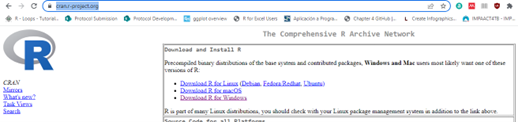
\includegraphics[keepaspectratio]{imagenes/01rwebpage.png}}

}

\caption{En esta página trata de descargar la versión más actualizada}

\end{figure}%

Luego de descargarlo puedes instalarlo inmediatamente usando el
ejecutable (para Windows y macOS) o la forma como se instalan software
in Linux. Para este manual estamos en un ambiente de Windows, luego de
instalar podemos acceder a la \textbf{\emph{consola}} de R (una pantalla
con un cursor parpadeando donde podemos escribir)

\begin{figure}[H]

{\centering \pandocbounded{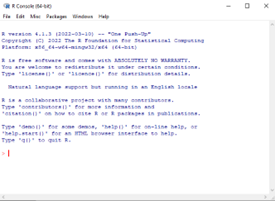
\includegraphics[keepaspectratio]{imagenes/01consolar.png}}

}

\caption{Este es la consola de R, aquí podemos comenzar a usar R, pero
es un poco complejo usar solamente la consola}

\end{figure}%

Aunque ya hayamos instalado R, al menos que seamos muy expertos en su
uso, que conozcamos bien las sintaxis de las funciones, que
\textbf{\emph{objetos}} (más tarde veremos lo que son los objetos) están
cargados en la memoria, entre otras cosas (¡también se puede usar como
una simple calculadora!), es muy complicado usar solamente la consola,
por lo que tenemos disponible aditamentos o accesorios que nos permiten
trabajar más fácil con R, así como su aprendizaje. Para este manual el
aditamento que usaremos es \textbf{Rstudio} de
\href{https://posit.co/}{Posit®}.

\subsection{Descargar e instalar
Rstudio}\label{descargar-e-instalar-rstudio}

Ahora vamos a instalar Rstudio, para esto vamos a descargarlo de la
siguiente página web,
\href{https://posit.co/download/rstudio-desktop/}{Descarga de Rstudio}
donde vamos a buscar la versión gratuita de escritorio para para el
sistema operativo que estamos usando.

En caso de que estés usando Linux, están las instrucciones en la página
de como hacerlo, la versión de Windows y macOS es un ejecutable.

Luego de descargar la ultima versión disponible procedemos a instalar
Rstudio, haciendo clic en el ejecutable, la instalación (en la versión
de Windows por ejemplo) es muy similar a cualquier otro software que
donde te pregunta el lugar donde será instalado y varias ventanas donde
se ve el progreso de instalación. Si todo salió bien, es decir que se
instaló sin errores, pues tendremos disponible en la barra de acceso
directo y en el escritorio, (si elegimos esta opción durante la
instalación) también tendremos un acceso directo.

Si tienes Windows, te compartimos el paso a paso en
\href{https://www.youtube.com/watch?v=M1iibA3gou8}{este video} para
descargar e instalar R y también R Studio Desktop.

\begin{figure}[H]

{\centering \pandocbounded{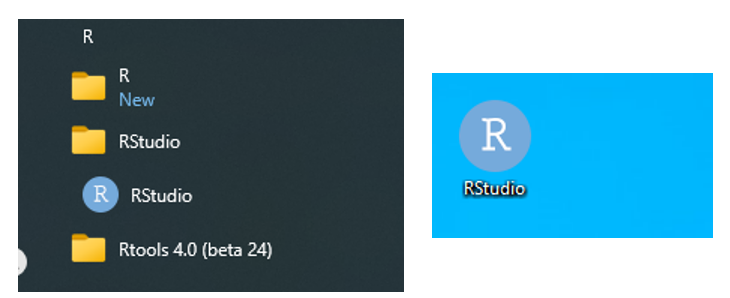
\includegraphics[keepaspectratio]{imagenes/01conorstudio.png}}

}

\caption{En Windows, la barra de inicio o las aplicaciones y si se creó
el acceso directo (derecha) en el escritorio}

\end{figure}%

Otro software que se debe instalar si el sistema operativo que usas es
Windows es \textbf{rtools}, dado que algunos paquetes necesitan que esté
instalado para funcionar de forma correcta.

Este se adquiere desde la página de
\href{https://cran.r-project.org/bin/windows/Rtools/}{Descarga rtools} y
elige la versión más reciente y descarga el formato ejecutable (termina
en ``installer'') en cualquier unidad de almacenamiento. Su instalación
sencilla, solo ejecutar el programa y hacer clic en siguiente las veces
que sea necesario.

\begin{figure}[H]

{\centering \pandocbounded{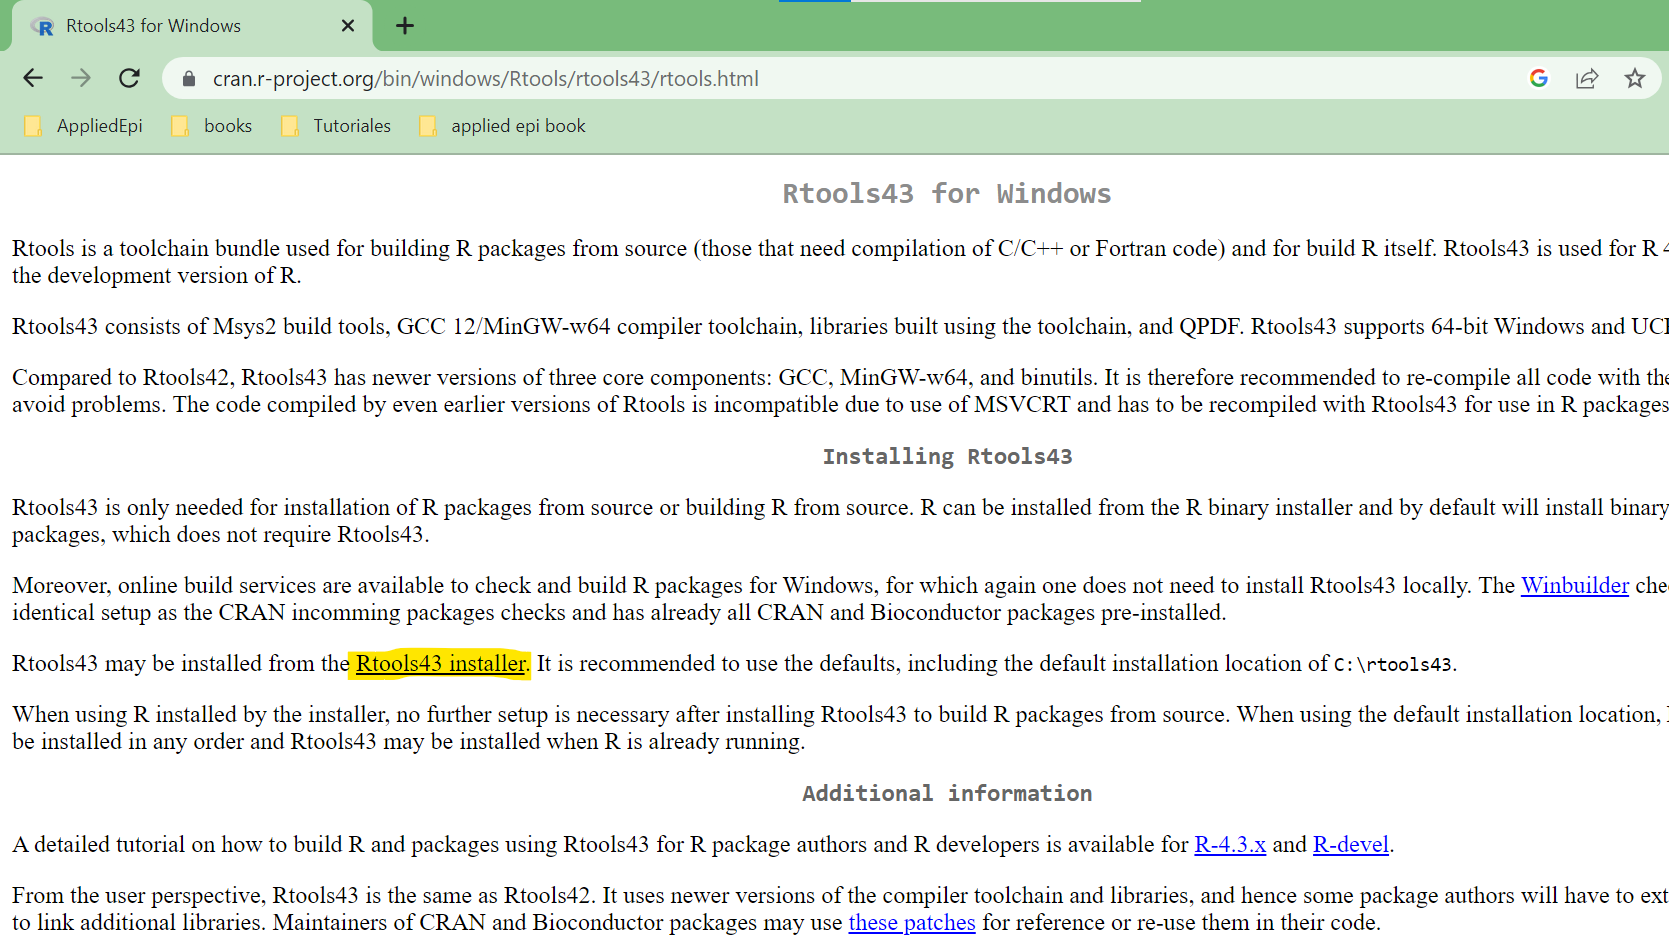
\includegraphics[keepaspectratio]{imagenes/01rtools.png}}

}

\caption{Busca esta version señalada en la imagen}

\end{figure}%

\section{Interfaz de Rstudio®}\label{interfaz-de-rstudio}

Para facilitar el aprendizaje y uso de R, vamos a usar RStudio que es un
entorno de desarrollo integrado o IDE (Integrated Development
Environment) y tiene la gran ventaja de que hay mucha documentación
sobre su uso, es muy cómoda de trabajar porque nos ayuda con la
escritura de los códigos, la organización de los archivos, tiene varios
visores o paneles para ver los códigos, las salidas, los objetos
cargados y otras ayudas más (Figura 5). RStudio ha permitido la difusión
del uso de R, lo que ha permitido la propagación de su uso en todas las
áreas donde se hace análisis de datos.

\begin{figure}[H]

{\centering 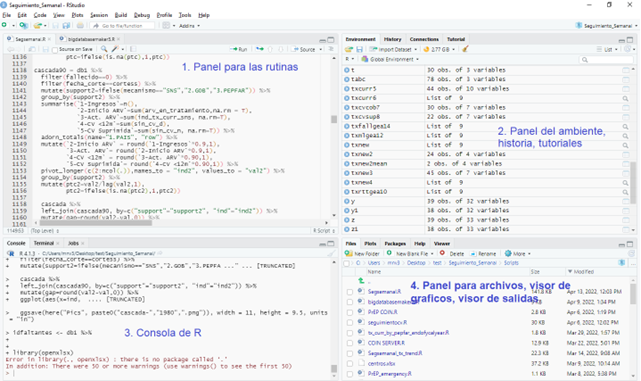
\includegraphics[width=6.6875in,height=\textheight,keepaspectratio]{imagenes/01interfazrstudio.png}

}

\caption{En esta imagen podemos ver los 4 paneles principales y el menú
de la interfaz de Rstudio}

\end{figure}%

\begin{enumerate}
\def\labelenumi{\arabic{enumi}.}
\item
  \textbf{Panel de las rutinas:}~este panel es el editor de texto donde
  vamos a escribir los códigos (rutinas) que vamos a usar para nuestras
  tareas, como las tablas, los gráficos, etc., que son automáticamente
  ejecutadas en la consola de R. Cada rutina se puede guardar como un
  archivo (muy similar a un archivo de texto normal), la característica
  más importante de este panel es que nos permite ver si el código tiene
  errores, pues a veces la falta de una simple coma o un caracter nos
  arroja error cuando ejecutamos comandos. También nos ofrece la
  herramienta de autocompletar y nos facilita mucho la organización del
  código. Para ejecutar una línea de código simplemente ponemos el
  cursor al inicio o al final de la línea y presionamos Ctrl+Enter o en
  el botón ``run'', mientras que para ejecutar la rutina completa,
  hacemos clic en el botón ``source''. Más adelante veremos varios
  ejemplos.
\item
  \textbf{Panel del ambiente} de trabajo \textbf{o panel de objetos
  cargados:} en este panel podemos ver cuales objetos tenemos cargados
  en la memoria del sistema, y nos permite ver qué tipo de objeto es (si
  es un \emph{dataframe}, un \emph{vector}, una \emph{matriz}, una
  \emph{función}, una l\emph{ista}). Esto nos ayuda a seguir el trabajo
  que vamos realizando, por ejemplo, cuando cargamos una base de datos
  desde un archivo de Excel en un objeto \emph{dataframe} podemos ver
  cuantas filas y variables tiene el archivo. También a través de este
  panel podemos salvar la sesión de trabajo, esto es útil cuando hacemos
  una pausa y queremos retomar más adelante lo que estábamos haciendo.
\item
  \textbf{Consola de R:} este es el lugar donde ocurre todo, puedes
  directamente escribir los comandos, las funciones, etc., pero para
  esto tenemos el panel de las rutinas, aquí también vas a ver los
  mensajes de errores cuando ejecutas una rutina o un comando, y por
  cada línea que se escribe se presiona ``enter'' para ejecutar los
  comandos. La ventaja más grande de utilizar RStudio es que hasta en la
  consola te identifica si hay errores o comandos incompletos y
  autocompletar.
\item
  \textbf{Panel para archivos, visor de gráficos y de salidas:} en este
  panel tenemos varias ventanas donde nos permite ver los archivos
  disponibles (muy parecido al explorador de Windows o a la carpeta de
  Documentos de tu computadora). A través del menú de este panel podemos
  crear carpetas, borrar, mover o copiar archivos, también podemos
  definir el directorio de trabajo (vamos a ver más adelante en detalle
  qué es el directorio o lugar de trabajo), a la derecha de Archivos o
  Files está el visor de gráficos (Plots), que podemos ampliar y poder
  copiar el gráfico que se está presentando y más a la derecha está el
  visor de salidas (Viewer), como tablas y datos en formato HTML.
  También en este panel está la ventana para instalar paquetes (término
  muy importante que lo veremos más adelante) y la ventana de ayuda
  (Figura 6).

  \begin{figure}[H]

  {\centering 
\includegraphics[width=5.32292in,height=\textheight,keepaspectratio]{imagenes/01figura06.png}

  }

  \caption{Figura 6.}

  \end{figure}%
\end{enumerate}

Antes de comenzar a trabajar puedes ir familiarizándote con esta
interface. En RStudio hay muchas opciones que iremos explicando en la
medida que vayamos avanzando, mientras tanto, te mostrados dos
herramientas interesantes del menú principal de RStudio: \textbf{Tools}
y \textbf{Help}.

Si vas al menú principal de RStudio, puedes entrar en la sección que
dice~\textbf{``Tools''} y dentro del menú desplegable seleccionas la
opción de \textbf{``Global Options''}~(al final del menú desplegable),
allí encontrarás un menú, y dentro de ``\textbf{Appearance}'' está la
opción ``Editor theme'' donde podrás cambiar los colores y el tipo de
letra de las ventanas, así podrás para adaptar el ambiente a tu gusto.
En Ayuda (Help) puedes encontrar los accesos directos para usar el
teclado, por ejemplo, salvar la rutina en la que estás trabajando,
reiniciar R, ejecutar toda la rutina, entre otros atajos. En la Figura 7
te mostramos cómo llegar a cada una de estas herramientas.

\begin{figure}[H]

{\centering 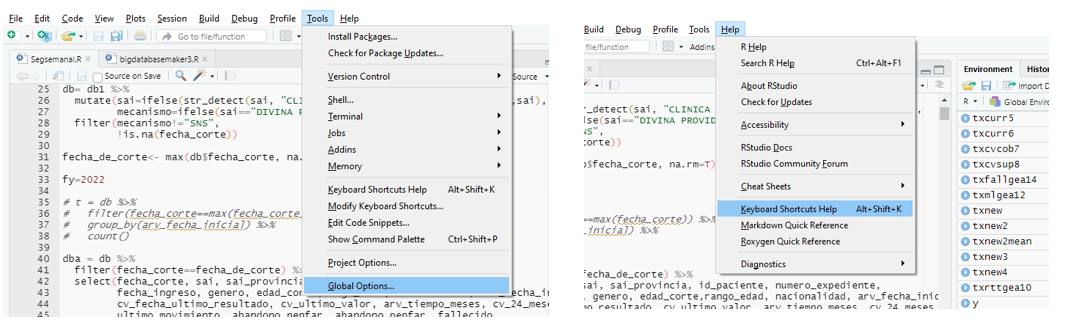
\includegraphics[width=8.48in,height=\textheight,keepaspectratio]{imagenes/01menurstudio.png}

}

\caption{Figura 7. Seleccionar ``Tool'' luego ``Global Options'' y en
ayuda, buscar los atajos del teclado}

\end{figure}%

\section{Instalación de Paquetes (librerías de
funciones)}\label{instalaciuxf3n-de-paquetes-libreruxedas-de-funciones}

Los paquetes son extensiones para añadir más funcionalidades a R. Es
quizás la razón por la cual R es ahora mismo una de las mejores
herramientas para trabajar con datos dada la cantidad de paquetes
específicos para realizar tareas como hacer tablas por ejemplo. En la
literatura, los paquetes se identifican con \{ \}, ejemplo: (Wickham and
RStudio 2023)\textbf{\{tidyverse\}} y los logos son una figura dentro de
un hexágono.

Con respecto a la instalación de paquetes, usualmente estos deben estar
publicados en CRAN (\href{https://cran.r-project.org/web/packages/}{Aquí
el enlace}) y se instalan desde el panel de paquetes (``Packages'').

\pandocbounded{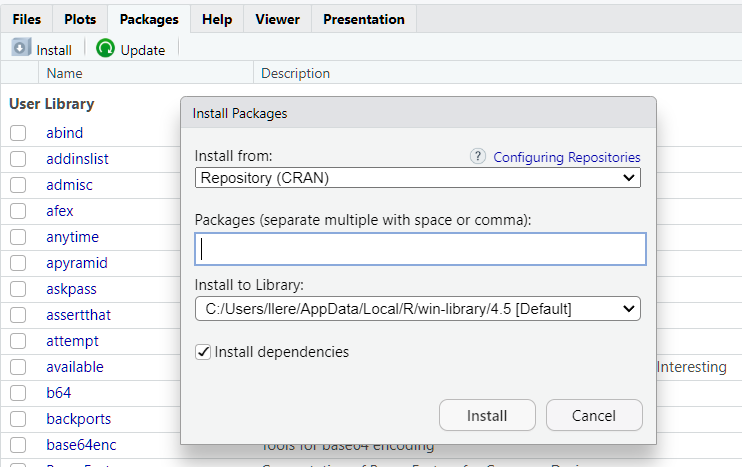
\includegraphics[keepaspectratio]{imagenes/01packages3.png}}

\section{Como instalar y cargar un paquete en
R}\label{como-instalar-y-cargar-un-paquete-en-r}

Después de instalar R, Rstudio solo tenemos las funcionalidades que trae
\textbf{R base}, que nos permiten hacer muchas cosas sin tener que
instalar nada más, pero podemos hacer que R sea más completo, ahora
vamos a ver que es un paquete y su importancia.

Como R es un lenguaje de programación por lo tanto podemos crear
programas o conjunto de funciones y estos programas podemos exportarlos
para luego usarlos más adelante.

Estos programas o complementos aumentan la capacidad de R a través de
funciones o comandos, por ejemplo, \textbf{R base}, no nos permite
exportar directamente los resultados o salidas en formato Excel o crear
tablas con formato de forma directa. Por lo tanto, los paquetes o
subprogramas hacen que R sea más que solo un lenguaje de programación.

Hay paquetes creados por epidemiólogos, para epidemiólogos como el
\{\textbf{epitools\}} (Aragon et al. 2020) o \{\textbf{epikit\}} (Spina
et al. 2023) que nos permiten con pocos comando o funciones hacer tareas
como calcular medidas de asociación (OR, Riesgo relativo) y facilitar
los análisis en epidemiología y otros paquetes que hacen las tareas de
análisis de datos como son el \{\textbf{openxlsx\}} (Schauberger et al.
2023) para manipular y crear archivos de Excel o el muy famoso y
aclamado paquete \textbf{tidyverse} (Wickham and RStudio 2023)del cual
hay este paquete hay libros escritos para el procesamiento y manejo de
datos por mencionar algunos.

Los paquetes nos permiten mejorar sobremanera nuestra productividad en
general. Cada vez que iniciamos una sesión con Rstudio, en nuestras
rutinas debemos cargar los paquetes que vamos a usar.

Dado que R es una plataforma colaborativa, cuando un paquete es creado
pasa por un proceso de validación antes de ser publicados en el
repositorio de R. Es por esto que, para su instalación debemos saber si
están disponibles. Los paquetes, usualmente, después de ya ser
validados, son publicados en el repositorio de R (The Comprehensive R
Archive Network o \href{https://cran.r-project.org/web/packages/}{CRAN})
que es la página donde descargamos R. También pueden estar disponibles
en otras páginas donde podemos descargarlos e instalarlos manualmente.
Después de instalar un paquete solo es necesario verificar si ha sido
actualizado, tal como haces con cualquier otro programa.

Usualmente los autores de los paquetes tienen tutoriales o páginas
llamadas ``Vignettes'' o viñetas donde podemos ver las funcionalidades y
tutoriales. Por ejemplo, ejemplo ingresa en la barra de búsqueda en tu
explorador estas palabras: ``R package epitools'', y aparecerán muchos
resultados para diferentes tareas. Sigue estos pasos para verificar si
un paquete existe buscando directamente desde RStudio:

\begin{enumerate}
\def\labelenumi{\arabic{enumi}.}
\tightlist
\item
  Ir al panel de archivos
\item
  Hacer clic en la ventana de paquetes o ``Packages''
\item
  Hacer clic en ``install''. Aparecerá una ventana donde escribirás el
  nombre del paquete. Si el paquete existe en CRAN, aparecerá en un
  listado y lo seleccionarás
\item
  Hacer clic en ``install''.
\end{enumerate}

\begin{figure}[H]

{\centering \pandocbounded{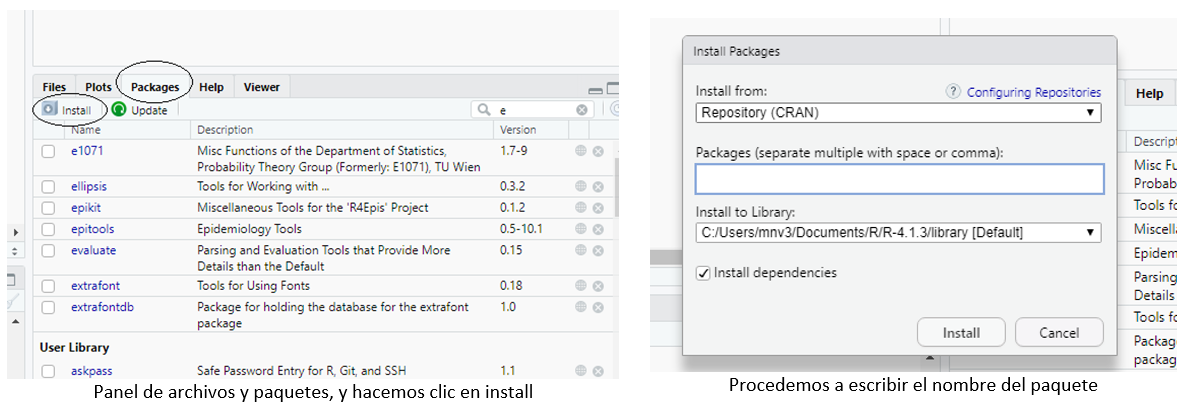
\includegraphics[keepaspectratio]{imagenes/01packages.png}}

}

\caption{installando un paquete en Rstudio}

\end{figure}%

Si el paquete no está disponible en CRAN pero si en la web y podemos
descargarlo y cambiar donde dice \textbf{``install from''} a
\textbf{``package archive file''} y buscar en el disco duro y proceder a
instalar (es muy raro que se de este caso y los paquetes que vamos a
instalar todos están disponible en CRAN).

La otra forma de instalar los paquetes es directamente desde la consola
o en un archivo de rutina usando el la función
\textbf{\emph{install.package()}} donde escribimos entre comillas el
nombre del paquete que queremos instalar.

\begin{figure}[H]

{\centering \pandocbounded{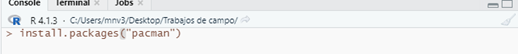
\includegraphics[keepaspectratio]{imagenes/01packages2.png}}

}

\caption{Figura 14. En esta imagen vemos en la consola la función para
instalar el paquete pacman}

\end{figure}%

Luego de esta introducción sobre qué es un paquete y cómo se instala,
vamos a hacer el siguiente ejercicio de instalar varios paquetes que
usaremos de forma constante en los ejercicios y tareas contenidos en
este manual. Ya sea directamente en la consola (ver imagen anterior), o
a través del panel de archivos, vamos a instalar este
paquete~\textbf{``pacman''}~(Tyler Rinker)~que es un paquete para
manejar paquetes y nos ahorrará muchos pasos, por ejemplo, detecta si un
paquete necesario está instalado o no, y procede a instalarlo, o ayuda a
instalar paquetes desde otras fuentes alternativas a CRAN. Después de
instalarlo podemos ver en la consola el mensaje de que se instaló
correctamente~ \textbf{(\emph{package `pacman' successfully unpacked and
MD5 sums checked}).}

En la rutina que comenzamos hace un momento atrás vamos a hacer la
siguiente tarea:

\begin{itemize}
\tightlist
\item
  Escribe o copia y pega el siguiente comando (recuerda, para ejecutar
  un comando o varios selecciona estos y presiona Ctrl+Enter o clic en
  ``Run''):
\end{itemize}

\begin{Shaded}
\begin{Highlighting}[]
\NormalTok{pacman}\SpecialCharTok{::}\FunctionTok{p\_load}\NormalTok{(}\StringTok{"tidyverse"}\NormalTok{, }\StringTok{"janitor"}\NormalTok{, }\StringTok{"gtsummary"}\NormalTok{, }\StringTok{"epikit"}\NormalTok{,}\StringTok{"here"}\NormalTok{,                }\StringTok{"epitools"}\NormalTok{, }\StringTok{"lubridate"}\NormalTok{, }\StringTok{"openxlsx"}\NormalTok{, }\StringTok{"readxl"}\NormalTok{, }\StringTok{"rio"}\NormalTok{)}
\end{Highlighting}
\end{Shaded}

Espera un momento si es la primera vez que se ejecuta para que así se
instalen los paquetes que están en el comando.. Antes de continuar,
vamos a explicar el comando anterior:

En Rstudio, en el editor de rutinas o en la misma consola, cuando
queremos ver las funciones o comandos disponibles en un paquete podemos
escribir el nombre del paquete seguido de dos puntos nos aparecerá una
ventana con un listado de dichas funciones, por ejemplo, este último
comando usamos el paquete \textbf{pacman} y dentro de este paquete
usamos la función de \textbf{\emph{p\_load}} (para cargar paquetes, que
también los instala si no están ya instalados)

\begin{figure}[H]

{\centering \pandocbounded{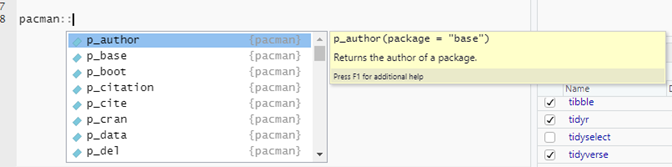
\includegraphics[keepaspectratio]{imagenes/01pacman.png}}

}

\caption{Esta es una de las funcionalidades de Rstudio que nos facilitan
el trabajo , luego de escribir el nombre del paquete y dos veces dos
puntos nos aparece el listado de funciones y también una ventana
amarilla para ayuda de la función presionando F1 para ver en el panel de
archivos, la ventana de ayuda y así ver los ejemplos de cómo usar dicha
función.}

\end{figure}%

Luego de escribir el nombre del paquete y dos veces dos puntos, nos
aparece el listado de funciones y también una ventana amarilla para
ayuda de la función, que también aparece presionando F1 o haciendo una
búsqueda en el panel de archivos en la ventana de ayuda, donde también
se pueden ver los ejemplos de cómo usar las funciones.

Los paquetes que hemos instalado hasta este momento no los vamos a
detallar por ahora, sino que, en la medida que vayamos haciendo los
ejercicios, vamos a ir explicando para qué sirven a través de las
funciones que traen cada uno. Es oportuno señalar que, dentro de los
paquetes disponibles en R, existen paquetes útiles para facilitar el
proceso de importar y exportar funciones específicas para las tareas del
epidemiólogo, para hacer reportes y para facilitar el proceso de la
gestión de los datos.

Para ver que paquetes tenemos cargados podemos escribir en la consola
\textbf{\emph{search()}}

\begin{Shaded}
\begin{Highlighting}[]
\FunctionTok{search}\NormalTok{()}
\end{Highlighting}
\end{Shaded}

\begin{verbatim}
 [1] ".GlobalEnv"        "package:rio"       "package:readxl"   
 [4] "package:openxlsx"  "package:epitools"  "package:here"     
 [7] "package:epikit"    "package:gtsummary" "package:janitor"  
[10] "package:lubridate" "package:forcats"   "package:stringr"  
[13] "package:dplyr"     "package:purrr"     "package:readr"    
[16] "package:tidyr"     "package:tibble"    "package:ggplot2"  
[19] "package:tidyverse" "package:stats"     "package:graphics" 
[22] "package:grDevices" "package:utils"     "package:datasets" 
[25] "package:methods"   "Autoloads"         "package:base"     
\end{verbatim}

Los dos capítulos siguientes son muy importantes. Debes familiarizarte
con ellos porque son los fundamentos para poder trabajar en R, veremos
ejemplos de las sintaxis de las expresiones, los diferentes tipos de
objetos de datos, y a medida que vayamos practicando se irá haciendo más
fácil entender el código, las funciones y las operaciones que hacemos.
Te recomendamos que, aparte de este manual, abundes más sobre los temas
que verás a continuación para que agilices tu proceso de aprendizaje con
R.

\bookmarksetup{startatroot}

\chapter{Comenzar a trabajar con R y la interfaz de
Rstudio}\label{comenzar-a-trabajar-con-r-y-la-interfaz-de-rstudio}

Ya luego de tener todo lo necesario instalado, ahora vamos a realizar
los siguientes pasos con la finalidad de ir aprendiendo a organizar los
trabajos que estaremos haciendo, como son los productos o asignaciones
que se deben hacer durante la capacitación, como son los análisis de
vigilancia, análisis de brotes, evaluación de sistema de vigilancia
entre otros.

Una gran recomendación es tener lo más organizado posible cada elemento
hecho en R o cualquier documento asociado a los análisis o trabajos que
vas a realizar; esto porque en nuestro caso, cuando comenzamos a
trabajar con RStudio guardábamos las rutinas y las salidas en diferentes
lugares, como principiantes al fin, no teníamos una estructura, y luego
cuando necesitábamos re-usar una rutina, buscar un documento de salida
era muy difícil de encontrar y perdíamos tiempo en esa búsqueda, a veces
nos tomaba más que lo que se toma ejecutar una rutina. Luego aprendimos
sobre lo que vamos a ver a continuación en cuanto a trabajar bajo
proyectos en RStudio.

\section{Creación de un proyecto}\label{creaciuxf3n-de-un-proyecto}

El primer paso para comenzar es decidir dónde estarán los archivos
relacionados al o a los trabajos que se van a hacer, es decir, debes
definir si almacenarás tu trabajo en un disco dentro de la PC o en la
``Nube'' (ejemplo, OneDrive, Google drive) para que así siempre
facilites tu trabajo, especialmente cuando necesites hacer cambios o
actualizar las bases de datos.

Esto es sumamente importante dado que nos ayudará a mantenernos
organizados. Todos los archivos como las bases de datos, las
referencias, las rutinas, deben estar almacenados en un lugar donde te
sea fácil encontrarlos y también para la ejecución o desarrollo del
proyecto o proyectos en que estés trabajando.

Para el segundo paso vamos a entrar en RStudio y vamos a crear un
\textbf{archivo de proyecto} de la siguiente forma:

\begin{figure}[H]

{\centering 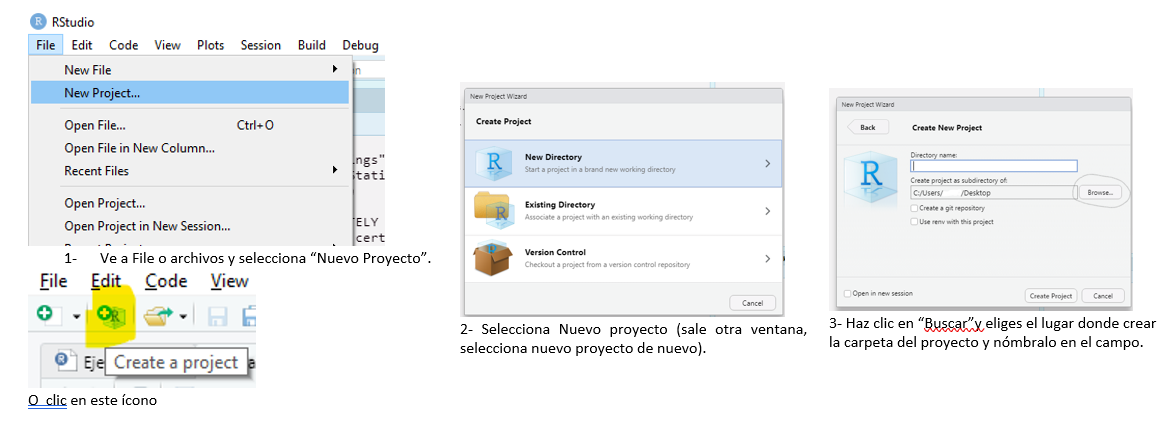
\includegraphics[width=6.18in,height=\textheight,keepaspectratio]{imagenes/01proyectonuevo.png}

}

\caption{Figura 10. Creando un proyecto}

\end{figure}%

\begin{enumerate}
\def\labelenumi{\arabic{enumi}.}
\item
  Crea el proyecto llamándolo ``mi\_primer\_proyecto'' siguiendo los
  pasos de la Figura 10.
\item
  Guarda el proyecto nuevo en el ``escritorio'' o en ``Documentos'' si
  usas Windows.
\item
  Para crear las carpetas, en la ventana inferior derecha o panel para
  archivos, ve a ``Archivos'' o ``File'', luego haz clic en ``new
  folder'' para crear las siguientes carpetas:
\end{enumerate}

\begin{enumerate}
\def\labelenumi{\alph{enumi}.}
\item
  ``Base de datos'' para almacenar tus datos en cualquier formato, como
  datos en Excel, por ejemplo.
\item
  ``Rutinas'' para salvar las rutinas que irás creando.
\item
  ``Referencias'' vas a poner aquí los documentos de soporte como
  referencias, artículos, etc.
\item
  ``Salidas'', donde vamos a salvar los documentos generados a partir de
  las rutinas, en esta última podemos tener una subcarpeta que se llame
  ``imágenes'' para las salidas que son imágenes, como gráficos o tablas
  salvadas en formato de imagen.
\end{enumerate}

\begin{figure}[H]

{\centering 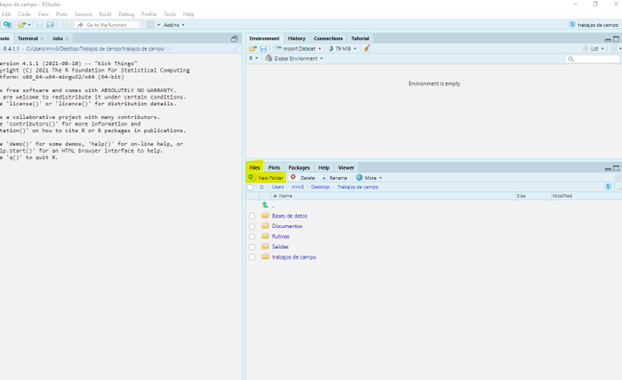
\includegraphics[width=6.19in,height=\textheight,keepaspectratio]{imagenes/01rstudiointerfazinicial.png}

}

\caption{Al finalizar, tu panel de archivos se tendría que ver como se
muestra en la Figura 11}

\end{figure}%

Si has hecho todos estos pasos y tu pantalla se parece a la imagen
anterior es porque has creado un proyecto. Puede verificar el nombre del
proyecto en la esquina superior derecha de la interfaz de RStudio.

Aparte de mantener una organización para mantener todo en orden, la
mayor ventaja de usar proyectos es que a RStudio se le facilita
encontrar dónde están los archivos que serán usados, por ejemplo, si
ubicas las bases de datos correctamente, será más fácil para ti importar
los datos a R y también exportar archivos a otras herramientas de
análisis.

\textbf{\emph{¿Por qué en la imagen anterior falta un panel}}

En la imagen anterior solo vemos 3 ventanas porque no hemos abierto o
creado una rutina, solo tenemos la consola, el panel del ambiente de
trabajo y el panel de archivos.

\section{Archivos de rutina (script) en
R}\label{archivos-de-rutina-script-en-r}

Siguiendo la secuencia de pasos para comenzar a trabajar con R en
Rstudio, vamos a ver uno de los elementos más importantes que son las
rutinas y que la usaremos constantemente.

Hasta este punto, hemos mencionado varias veces la palabra ``rutina''.
Una rutina no es más que un ``documento'' donde escribimos comandos
(funciones, cálculos, etc.), que puede ser ejecutado las veces que sea
necesario (como por ejemplo procesar y generar un reporte semanal).
Realmente crear una rutina es un procedimiento muy sencillo porque se
trata simplemente de escribir en un editor de texto las funciones que
generan los resultados que esperamos.

Dado que podemos salvar las rutinas como archivos, podemos compartirlas
y guardarlas para luego usarlas como referencia.

Para crear una nueva rutina en RStudio vamos a \textbf{\emph{``file''
-\textgreater{} ``new file'' -\textgreater{} ``R Script''}} (en inglés
rutina es igual a \textbf{\emph{Script}} por lo que estaremos utilizando
ambos conceptos de manera indistinta a lo largo del curso).

Después de aceptar ahora tenemos el panel de rutinas habilitado (igual
que un editor de texto) tal como se ilustra en la Figura 12.

Cuando salves la rutina nueva por primera vez, te pedirá dónde guardar
el archivo, entonces procede a guardarlo en la carpeta de ``Rutinas''
que previamente creaste en el Panel de archivos y ya podrás comenzar a
trabajar. Es importante anotar que RStudio no salva el avance de tu
rutina automáticamente, sino que siempre debes guardar cada cierto
tiempo, ya sea a través del menú o utilizando el atajo \textbf{Ctrl+S}.

\begin{figure}[H]

{\centering \pandocbounded{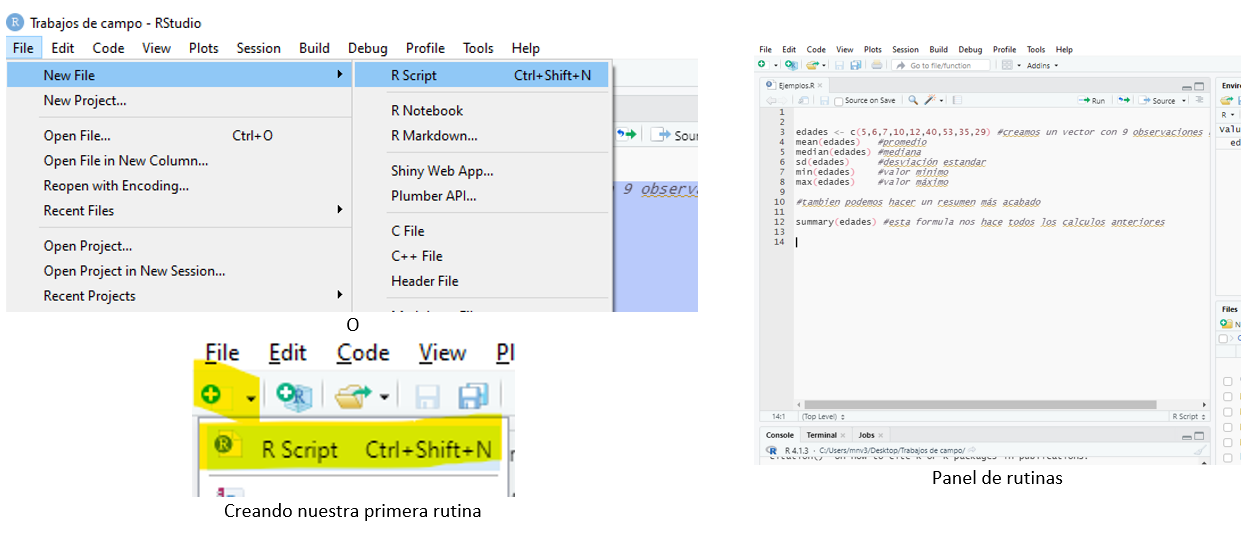
\includegraphics[keepaspectratio]{imagenes/01rutina.png}}

}

\caption{Figura 12. Pasos para comenzar un archivo de rutinas o
(Ctrl+Shift+N)}

\end{figure}%

Si has llegado hasta aquí, entonces ya tienes una gran parte del camino
recorrido, es decir, ya tienes el programa instalado y disponible, un
proyecto creado y tu primera rutina guardada. Si desde ya comenzáramos a
trabajar, podemos escribir comandos directamente en la consola o en el
documento de la rutina para hacer operaciones como aplicar a nuestros
datos los \textbf{estadísticos de tendencia central}, para que vayas
viendo y familiarizándote con R. Vamos a hacer la siguiente prueba paso
a paso:

\begin{enumerate}
\def\labelenumi{\arabic{enumi}.}
\tightlist
\item
  Escribe el texto debajo en el documento de la rutina, o si estas desde
  tu PC, copia y pega todo este texto, selecciónalo (como en cualquier
  editor de texto o Ctrl+A) y presiona \textbf{Ctrl+Enter} o haz clic en
  \textbf{``Run''}.
\end{enumerate}

\begin{Shaded}
\begin{Highlighting}[]
\NormalTok{edades }\OtherTok{\textless{}{-}} \FunctionTok{c}\NormalTok{(}\DecValTok{5}\NormalTok{,}\DecValTok{6}\NormalTok{,}\DecValTok{7}\NormalTok{,}\DecValTok{10}\NormalTok{,}\DecValTok{12}\NormalTok{,}\DecValTok{40}\NormalTok{,}\DecValTok{53}\NormalTok{,}\DecValTok{35}\NormalTok{,}\DecValTok{29}\NormalTok{) }\CommentTok{\#creamos un vector con 9 observaciones numericas }
\FunctionTok{mean}\NormalTok{(edades)   }\CommentTok{\#promedio }
\FunctionTok{median}\NormalTok{(edades) }\CommentTok{\#mediana }
\FunctionTok{sd}\NormalTok{(edades)     }\CommentTok{\#desviación estandar }
\FunctionTok{min}\NormalTok{(edades)    }\CommentTok{\#valor minimo }
\FunctionTok{max}\NormalTok{(edades)    }\CommentTok{\#valor máximo  }
\CommentTok{\#tambien podemos hacer un resumen más acabado, con menos comandos }
\FunctionTok{summary}\NormalTok{(edades) }\CommentTok{\#esta función nos hace todos los calculos anteriores\}}
\end{Highlighting}
\end{Shaded}

\begin{enumerate}
\def\labelenumi{\arabic{enumi}.}
\setcounter{enumi}{1}
\tightlist
\item
  Luego de ejecutar los comandos, podemos ver el resultado en la
  consola. Como puedes observar, está escrito lo mismo que la rutina
  pero debajo de cada comando hay un resultado, es decir, vas a ver el
  resultado de calcular el promedio a través de la función mean() cuyo
  resultado es 21.8, y así sucesivamente. La consoloa debería verse algo
  similar a esto:
\end{enumerate}

\begin{Shaded}
\begin{Highlighting}[]
\NormalTok{edades }\OtherTok{\textless{}{-}} \FunctionTok{c}\NormalTok{(}\DecValTok{5}\NormalTok{,}\DecValTok{6}\NormalTok{,}\DecValTok{7}\NormalTok{,}\DecValTok{10}\NormalTok{,}\DecValTok{12}\NormalTok{,}\DecValTok{40}\NormalTok{,}\DecValTok{53}\NormalTok{,}\DecValTok{35}\NormalTok{,}\DecValTok{29}\NormalTok{) }\CommentTok{\#creamos un vector con 9 observaciones numericas }
\FunctionTok{mean}\NormalTok{(edades)   }\CommentTok{\#promedio }
\end{Highlighting}
\end{Shaded}

\begin{verbatim}
[1] 21.88889
\end{verbatim}

\begin{Shaded}
\begin{Highlighting}[]
\FunctionTok{median}\NormalTok{(edades) }\CommentTok{\#mediana }
\end{Highlighting}
\end{Shaded}

\begin{verbatim}
[1] 12
\end{verbatim}

\begin{Shaded}
\begin{Highlighting}[]
\FunctionTok{sd}\NormalTok{(edades)     }\CommentTok{\#desviación estandar }
\end{Highlighting}
\end{Shaded}

\begin{verbatim}
[1] 17.73728
\end{verbatim}

\begin{Shaded}
\begin{Highlighting}[]
\FunctionTok{min}\NormalTok{(edades)    }\CommentTok{\#valor minimo }
\end{Highlighting}
\end{Shaded}

\begin{verbatim}
[1] 5
\end{verbatim}

\begin{Shaded}
\begin{Highlighting}[]
\FunctionTok{max}\NormalTok{(edades)    }\CommentTok{\#valor máximo  }
\end{Highlighting}
\end{Shaded}

\begin{verbatim}
[1] 53
\end{verbatim}

\begin{Shaded}
\begin{Highlighting}[]
\CommentTok{\#tambien podemos hacer un resumen más acabado, con menos comandos}
\FunctionTok{summary}\NormalTok{(edades) }\CommentTok{\#esta función nos hace todos los calculos anteriores}
\end{Highlighting}
\end{Shaded}

\begin{verbatim}
   Min. 1st Qu.  Median    Mean 3rd Qu.    Max. 
   5.00    7.00   12.00   21.89   35.00   53.00 
\end{verbatim}

Una de las ventajas que tiene RStudio de trabajar con los documentos de
rutina es que puedes tener varias rutinas abiertas a la misma vez y
navegar entre ellas. Esto te puede resultar útil para utilizar una
rutina dentro de otra, es decir, como las rutinas se pueden guardar en
la PC, vas a darte cuenta de que hay muchos procedimientos que se
repiten y que solo necesitas modificarlos levemente, en estos casos,
mientras estás haciendo una rutina puedes usar otra como referencia para
tomar códigos que ya has usado antes o que te han compartido.
\emph{¿Cuál es la ventaja de esto? ¡que no es obligatorio aprenderse
todas las funciones o comandos de R!}

Una muy buena práctica es comentar todo lo que haces para luego saber
qué hiciste en una secuencia de códigos. Para esto, solo tienes que
comenzar una línea con el carácter ``\#'' o signo de número, y todo el
texto después de este carácter cambia de color y se pone en formato
itálico, tornando el texto de color verde de forma predeterminada,
aunque el color verde pudiera variar dependiendo de la configuración de
colores que hayas elegido, tal como te explicamos en la sección 2.2.
Cuando estemos en los pasos de hacer tablas y gráficos, vamos a usar
mucho los comentarios.

El editor de texto de rutina en RStudio también nos permite ver si hay
errores en el código, otra de las tantas funcionalidades que nos ofrece
el programa para hacer más fácil la escritura de códigos.

\begin{figure}[H]

{\centering 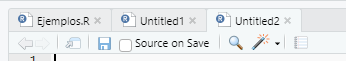
\includegraphics[width=0.5\linewidth,height=\textheight,keepaspectratio]{imagenes/01rutinas2.png}

}

\caption{Varias rutinas abiertas (con \textbf{Ctrl+shift+tab} podemos
movernos entre las rutinas sin usar el ratón)}

\end{figure}%

\bookmarksetup{startatroot}

\chapter{Operadores en R}\label{operadores-en-r}

Antes de continuar con los paquetes y funciones, debemos conocer algunos
conceptos básicos para poder trabajar con R. Se trata de los operadores,
los de uso común en matemáticas (como suma, resta, multiplicación y
división), los de asignación, los booleanos, entre otros. Es bueno que
sepas, si acaso no lo sabes, que todos los lenguajes de programación
usan operadores.

Los operadores son los que nos permiten escribir las expresiones que
usaremos en nuestras rutinas y las funciones. En R, hay operadores que
se usan constantemente para crear nuestro código.

Desde que abres R, puedes utilizarlo como una calculadora (muy avanzada,
por cierto), es decir, si escribes en la consola 2+2 y presionas
\textbf{Enter} tendrás un resultado, pero si queremos correr varias
veces esta misma operación podemos guardarla en un \textbf{objeto} y en
vez de escribir de nuevo la operación (el 2+2) podemos simplemente
llamar este \textbf{objeto} con solo escribirlo y vamos a obtener el
mismo resultado. manejar los objetos nos agiliza mucho el trabajo.

Dentro de las funciones podemos ver si un valor o un objeto está
presente, así como también reasignar un valor o hacer operaciones
matemáticas. A continuación, te mostramos los operadores que
utilizaremos con más frecuencia.

\subsection{\texorpdfstring{\textbf{Resumen de los operadores más usados
para la escritura de las expresiones en
R}}{Resumen de los operadores más usados para la escritura de las expresiones en R}}\label{resumen-de-los-operadores-muxe1s-usados-para-la-escritura-de-las-expresiones-en-r}

\begin{longtable}[]{@{}
  >{\raggedright\arraybackslash}p{(\linewidth - 6\tabcolsep) * \real{0.0223}}
  >{\raggedright\arraybackslash}p{(\linewidth - 6\tabcolsep) * \real{0.0318}}
  >{\raggedright\arraybackslash}p{(\linewidth - 6\tabcolsep) * \real{0.4793}}
  >{\raggedright\arraybackslash}p{(\linewidth - 6\tabcolsep) * \real{0.4634}}@{}}
\toprule\noalign{}
\begin{minipage}[b]{\linewidth}\raggedright
Tipo
\end{minipage} & \begin{minipage}[b]{\linewidth}\raggedright
Operador
\end{minipage} & \begin{minipage}[b]{\linewidth}\raggedright
Descripción
\end{minipage} & \begin{minipage}[b]{\linewidth}\raggedright
Ejemplo
\end{minipage} \\
\midrule\noalign{}
\endhead
\bottomrule\noalign{}
\endlastfoot
Asignación & \textless- & Para asignar un valor a un objeto (el signo de
= es similar) se compone de ``menor que'' seguido de una raya o ``dash''
& x \textless- 2+2 con esto creamos (asignamos) la operación 2+2 al
objeto x

si volvemos a usar x como objeto y le asignamos otro valor, este se
sobrescribirá \\
Asignación & '' '' & Las comillas son para declarar texto, si escribes
cualquier caracter entre comillas será reconocida como una cadena de
caracteres & z~ \textless- ``Me gusta R'' asignamos al objeto z el
texto \\
Evaluación & == & igual, igual significa Igual, para evaluar si un
objeto es igual a otro o una variable es igual a un valor & x ==4 (la
respuesta es TRUE) \\
Evaluación & != & Significa no es igual, para evaluar si un objeto es
diferente a otro o una variable es diferente a un valor. & x != 4 (la
respuesta es FALSE) \\
Evaluación & \textgreater, \textless, \textgreater=, \textless= & Signos
para evaluar mayor que, menor que, mayor o igual que y menor o igual
que, aparte de los números, estos operadores funcionan con texto, (b es
menor que c por ejemplo) & x\textless5 (la respuesta es TRUE),
x\textgreater5 (la respuesta es FALSE)

x\textgreater=3 (la respuesta es TRUE)

x\textless=5 (la respuesta es FALSE) \\
Evaluación & \%in\% & Identifica si un elemento (como un número, por
ejemplo) está dentro de un objeto (si queremos decir ``no esta incluido
en'' solo agregamos signo de exclamación !) & 2 \%in\% x (la respuesta
es TRUE)

2 !\%in\% x (la respuesta es FALSE) \\
Acceso & \$ & Signo de dinero sirve para acceder a las variables de un
dataframe o una lista & mtcars (un dataframe interno de R) tiene 11
columnas, para seleccionar o aplicar una función a una de estas (como
\textbf{mean} para promedio) escribes el nombre del dataframe seguido
del signo de dinero y el nombre de la variable así :
\textbf{mean(mtcars\$cyl)} para retornar el promedio o 6.1875 \\
Acceso & {[} {]} & Los corchetes son usados con los vectores, matrices y
dataframe para acceder a un valor en base de una posición (para las
matrices y dataframe) donde el primer valor es el numero de fila y el
segundo valor es el numero de columna. Para los vectores solo se usa un
valor para especificar la posción. & usando \textbf{mtcars} de nuevo, si
quiero saber que valor está en la fila 20 de la columna 3 puedes
escribir este código \textbf{mtcars{[}20,3{]}} y retorna 71.1 que es el
valor de la variable \textbf{disp} de la fila del carro toyota
corolla. \\
Booleano & \& & Y o AND & \textbf{y} = c(1,3,4,9,11,10) \#un vector con
6 elementos

3 \& 4 \%in\% y (la respuesta es TRUE, porque están ambos, si no es así,
es FALSE ) \\
Booleano & \textbar{} & O o OR & 3 \textbar{} 30 \%in\% y (la respuesta
es TRUE, porque está al menos 1 de los elementos dentro del objeto o
vector \textbf{y}, si ambos elementos faltaran, la respuesta seria
FALSE) \\
Aritméticos & +, -, *, /,\^{}, = & Signos matemáticos para suma, resta,
multiplicación, división y exponente. El igual es usado más para
asignación & 2*2 retorna 4

2+2 retorna 4

4/2 retorna 2

x = 2+2 (igual como asignación, otro ejemplo x\textbf{=}log(4),donde
log() es una función que la usamos para asignar al objeto x el logaritmo
de 4) \\
Otros & ( ) & Los paréntesis son símbolos que se usan mucho en
operaciones y funciones para determinar que ocurra algo y en el orden,
siempre desde los más internos hacia los externos & mean(c(3,4,5,6,2,5))
el resultado es 4.16, si te fijas primero tenemos un set de paréntesis
que crea un objeto, luego el otro set de paréntesis que indica calcular
el promedio de este grupo usando la función \textbf{\emph{mean(),}} \\
Otros & \%\textgreater\% o ``pipe'' & Es un operador para indicar una
secuencia de comandos o expresiones que se realizan a partir de un
objeto en cascada, significa ``entonces o luego'' (vamos a ver más de su
uso cuando veamos transformación de datos) se puede escribir con Ctrl+M
y hay que tener instalado el paquete \textbf{tidyverse} &
c(3,4,5,6,2,5)\%\textgreater\%

mean() nos da el mismo resultado que

mean(c(3,4,5,6,2,5)), básicamente una expresión como esta nos dice
``crea un objeto de 5 numeros, \textbf{Entonces} (el pipe) obtén el
promedio'' \\
otros & , (comma) & La coma en R se usa para asignar un espacio de un
elemento o un parámetro, por ejemplo, el primer elemento luego una coma,
segundo elemento y luego una coma & y \textless- c(``a''\textbf{,}
``b''\textbf{,}''c'')

ggplot(data=df, aes(x=var1\textbf{,} y=var2\textbf{,} fill=cat1)) \\
\end{longtable}

En la medida que vayas practicando los operadores se irán haciendo
familiares y más fácil de entender. Siempre hay que tomar en cuenta que
un operador mal usado dará error cuando ejecutamos un comando o código,
verás que te ocurrirá a menudo dejar de escribir el último paréntesis, o
cerrar comillas.

\bookmarksetup{startatroot}

\chapter{Objetos en R}\label{objetos-en-r}

Otro elemento de suma importancia a conocer cuando se trabaja con R, así
como vimos la importancia de las rutinas, son los objetos y sus
diferentes tipos, dado que es con esto que trabajamos. Son básicamente
los contenedores de los datos, que R los almacena en la memoria del
computador, es decir, a partir de estos es que haremos nuestras salidas
como tablas, gráficos, reportes a través de la transformación (declarar,
nombrar, filtrar reemplazar), entre otras. Básicamente los objetos son
el fundamento de todo.

En R, hay 5 tipos de objetos de datos y se dividen en dos grupos de
objetos: los que son de un solo tipo de dato (atómicos) o los que tienen
varios tipos de datos (recursivos). Empecemos con los atómicos.

\section{Vectores}\label{vectores}

Dentro de los objetos atómicos tenemos \textbf{los vectores}, los cuales
no tienen dimensión, es decir, no están compuestos por filas o columnas
como un dataframe, y pueden ser de clase numérica (entero y decimal),
integer (números enteros solamente), caracter o texto, lógico (TRUE,
FALSE) y factor (jerarquía en los valores). Un ejemplo de creación de un
vector es el siguiente:

\pandocbounded{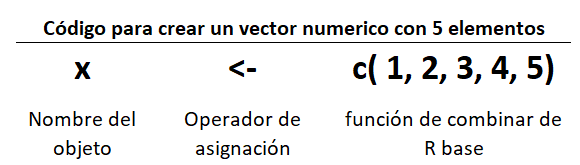
\includegraphics[keepaspectratio]{imagenes/05vector.png}}

\pandocbounded{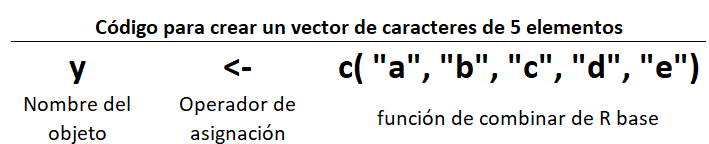
\includegraphics[keepaspectratio]{imagenes/05vector2.png}}

Para los vectores que son de \emph{caracteres o texto}, si al crearlos
les ponemos números sin comillas, cuando los llamemos serán reconocidos
como texto, por lo tanto, no se pueden hacer operaciones matemáticas con
estos vectores aunque sean números.

Si escribes ``x'' (o el nombre que hayas usado para crear el vector) y
presionas \textbf{Enter,} en la consola observaras los elementos
contenidos en este vector.

Una de las funcionalidades más interesantes de R es que, en el caso de
vectores numéricos, si haces una operación matemática como 5 +
\textbf{x} (nombre del vector), la operación se hará en todos los
elementos del vector, es decir, el 5 se sumará con cada uno de los
números. Si haces esto con un vector de texto o carácter, en la consola
observarás un error que es una operación entre un argumento no numérico
contra otro numérico.

A medida que avancemos con el desarrollo de los productos vamos a ver
que los vectores los usamos de forma constante; un ejemplo común es
crear un vector con los nombres de las provincias o municipios de
interés para luego poder hacer un filtro invocando dicho vector. También
se puede hacer combinando varios tipos de vectores con las mismas
dimensiones, es decir, el mismo número de elementos podemos ``unirlos''
y formar un nuevo objeto como un \textbf{dataframe} o una lista.

\section{Matrices}\label{matrices}

Otro tipo de objeto atómico o que solo admite un tipo de valor es
\textbf{la matriz} que es básicamente un vector pero con dos dimensiones
(columnas y filas) se crean usando la función \textbf{matrix()} y se le
debe agregar el parámetro del total de filas así como el total de
columnas por ejemplo de la siguiente forma:

\pandocbounded{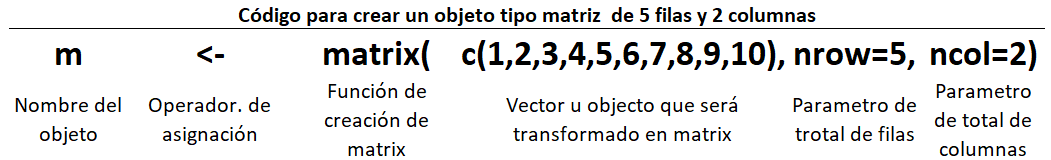
\includegraphics[keepaspectratio]{imagenes/05matrix.png}}

No entraremos detalles ahora con los objetos de tipo matriz porque estos
objetos tienen sus usos bien específicos y no vamos a usarlos de forma
constante como lo haremos con los vectores.

\section{Dataframes (conjunto de
datos)}\label{dataframes-conjunto-de-datos}

Ahora vamos a ver uno de los objetos más importantes que vamos a usar,
los \textbf{dataframes}, que es un objeto de tipo recursivo o que admite
varios tipos de datos (texto, numérico, lógico) y es idéntico a una
tabla, es decir, tiene dos dimensiones, columnas y filas. Las columnas
se pueden ver como si fueran variables y las filas son los valores
contenidos en esta variable.

Para los trabajos que vamos a realizar, este será el tipo de objeto con
el que más nos sentiremos familiarizados, dado que lo más parecido a un
dataframe es una base de datos, ya sea en Excel u otro tipo de programa.

Una de las ventajas que tiene Rstudio es que nos ayuda a ver fácilmente
la estructura del objeto dataframe, cuantas variables o columnas y
cuantas filas u observaciones contiene para visualizar el contenido.

\begin{figure}[H]

{\centering \pandocbounded{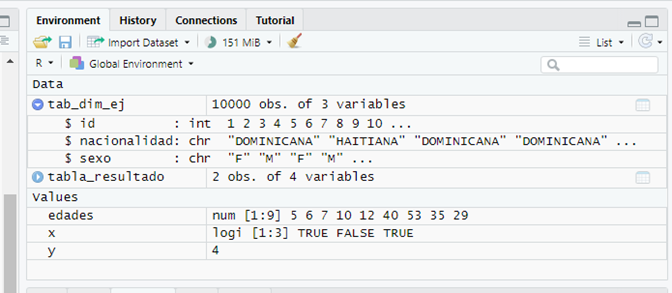
\includegraphics[keepaspectratio]{imagenes/05dataframe.png}}

}

\caption{Panel de ambiente de trabajo en Rstudio donde podemos ver los
objetos de datos disponibles, en esta imagen podemos ver dos dataframes
(tab\_dim\_ej y tabla\_resultado) y debajo, en la categoría de values, 3
vectores, (edades, x y ``y'') . Rstudio nos permite diferencial
rápidamente también ver los atributos de cada elemento. Para saber más
sobre los tipos de objetos podemos usar dos funciones str() y class(),
la primera para ver la estructura y la segunda para ver que clase de
objeto es.}

\end{figure}%

Para comenzar a usar los \textbf{dataframes} tenemos dos formas de
hacerlo. Primero, creándolo directamente escribiendo los datos que
usaremos, combinando varios vectores para crear una tabla como en el
siguiente ejemplo:

\begin{Shaded}
\begin{Highlighting}[]
\NormalTok{ var1 }\OtherTok{\textless{}{-}} \FunctionTok{c}\NormalTok{(}\StringTok{"maria"}\NormalTok{, }\StringTok{"pedro"}\NormalTok{, }\StringTok{"juan"}\NormalTok{, }\StringTok{"jose"}\NormalTok{) }\CommentTok{\#creamos un vector con nombres por ejemplo}
\NormalTok{ var2 }\OtherTok{\textless{}{-}} \FunctionTok{c}\NormalTok{(}\DecValTok{25}\NormalTok{, }\DecValTok{40}\NormalTok{, }\DecValTok{30}\NormalTok{, }\DecValTok{35}\NormalTok{) }\CommentTok{\#creamos otro vector con las edades}
\NormalTok{ var3 }\OtherTok{\textless{}{-}} \FunctionTok{c}\NormalTok{(}\StringTok{"F"}\NormalTok{, }\StringTok{"M"}\NormalTok{, }\StringTok{"M"}\NormalTok{, }\StringTok{"M"}\NormalTok{) }\CommentTok{\#creamos otro vector con el sexo}
\NormalTok{ var4 }\OtherTok{\textless{}{-}} \FunctionTok{c}\NormalTok{(}\StringTok{"LR"}\NormalTok{, }\StringTok{"SD"}\NormalTok{, }\StringTok{"SC"}\NormalTok{, }\StringTok{"PP"}\NormalTok{) }\CommentTok{\# creamos otro vector con la procedencia}
\NormalTok{ tabla }\OtherTok{\textless{}{-}} \FunctionTok{data.frame}\NormalTok{(}\AttributeTok{nombre=}\NormalTok{var1, }\AttributeTok{edad=}\NormalTok{var2, }\AttributeTok{sexo=}\NormalTok{var3, }\AttributeTok{prov=}\NormalTok{var4)}
 
\NormalTok{tabla}
\end{Highlighting}
\end{Shaded}

\begin{verbatim}
  nombre edad sexo prov
1  maria   25    F   LR
2  pedro   40    M   SD
3   juan   30    M   SC
4   jose   35    M   PP
\end{verbatim}

\begin{figure}[H]

{\centering \pandocbounded{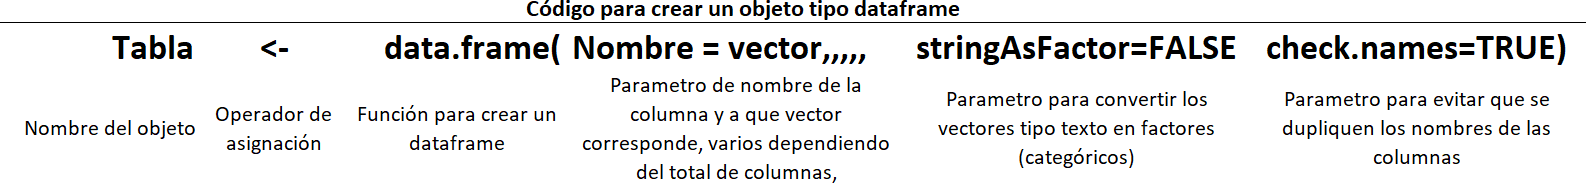
\includegraphics[keepaspectratio]{imagenes/05dataframe2.png}}

}

\caption{Anatomía de la función data.frame() para crear un dataframe. en
R las funciones vienen con valores en los parámetros de forma
predeterminada, incluso no hay que escribirlos. Un ejemplo es en esta
función de \textbf{data.frame()} el parámetro
\textbf{\emph{check.names=TRUE}} viene predeterminado y por ende no hay
que escribirlo.}

\end{figure}%

Entonces si ejecutamos las líneas anteriores vamos a tener como
resultado un dataframe nuevo con 4 variables y 4 observaciones.
\textbf{¡Ojo!} los vectores deben de tener la misma cantidad de
elementos, de lo contrario, veremos el siguiente error:
\textbf{\emph{``Error in data.frame(nombre = var1, edad = var2, sexo =
var3, prov = var4) : arguments imply differing number of rows: 4, 3'',}}
esto significa que uno de los vectores no tiene la misma cantidad de
elementos.

Para corregir esto, si el valor es desconocido en el vector que nos
falta un elemento, solo agregamos un elemento nuevo llamado
\textbf{\emph{NA,}} sin comillas, que es una forma de decirle a R que el
valor es desconocido, posteriormente, ejecutamos de nuevo las líneas
donde hicimos el cambio para actualizar ¡y listo!

Este abordaje puede ser útil para tablas pequeñas, pero cuando tenemos
que trabajar con bases de datos que tienen cientos o miles de
observaciones, entonces creamos un dataframe importando los datos desde
diferentes fuentes, como archivos de Excel, desde archivos de texto,
incluso archivos nativos de otros programas estadísticos como SPSS o
STATA.

En Rstudio podemos, sin necesidad de escribir una expresión o comando,
usar el botón de ``\textbf{import Dataset''} en el panel de ambiente de
trabajo, y al hacer clic, se despliega un menú para diferentes tipos de
formatos de bases de datos como Excel, csv, txt, SPSS, SAS o Stata.

\begin{figure}[H]

{\centering \pandocbounded{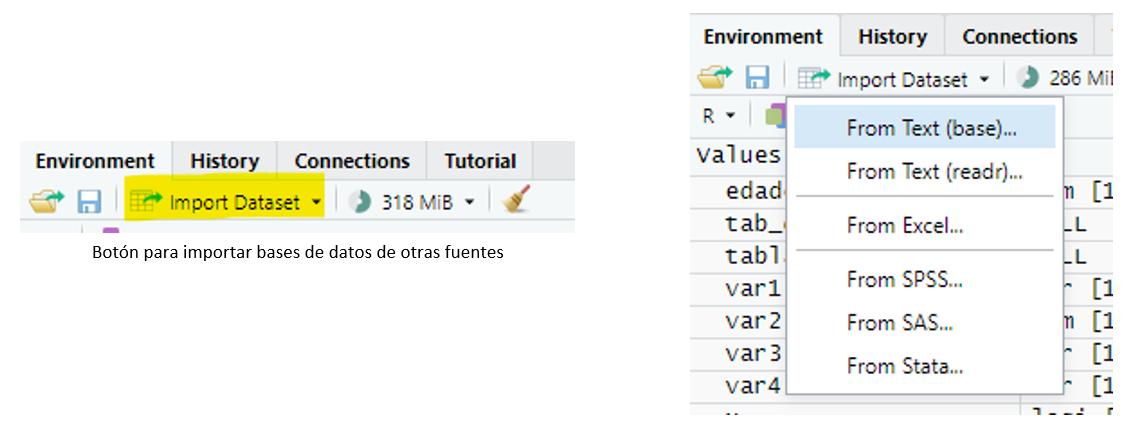
\includegraphics[keepaspectratio]{imagenes/05importdatagrame.png}}

}

\caption{Botón para importar bases de datos de otras fuentes}

\end{figure}%

Después de hacer clic en uno de los formatos, (ejemplo Excel) se abre
una ventana para seleccionar el archivo de la base de datos, que
variables o columnas vamos a incluir además de otros parámetros.

\begin{figure}[H]

{\centering \pandocbounded{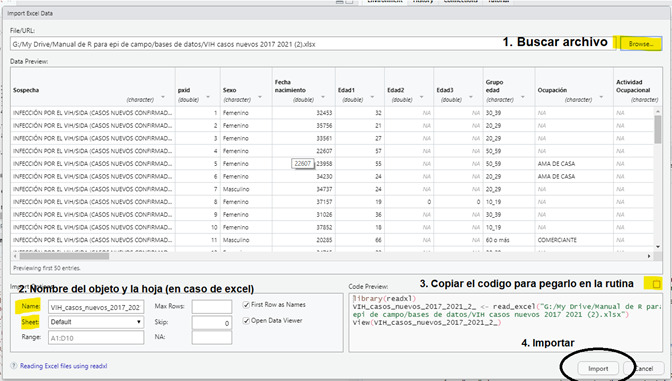
\includegraphics[keepaspectratio]{imagenes/05importdatagrame2.png}}

}

\caption{Pasos para importar un dataframe usando Rstudio}

\end{figure}%

De forma predeterminada, en el nombre del objeto o dataframe estará el
nombre del archivo de la base de datos, y puedes cambiarlo a un nombre
más amigable (ejemplo bd o base). Si estás usando un archivo de Excel
que contiene varias hojas, puedes especificar cual hoja usarás
en~\textbf{``sheet''}, incluso, puedes elegir el rango de filas que
usarás en caso de que no quieras seleccionar la hoja completa. De igual
manera, puedes poner desde cuál fila se leerá el archivo, esto es
importante si la base de datos en Excel tiene títulos y los datos se
comienzan a partir de la 3ra o 4ta fila, en este caso, puedes
en~\textbf{``skip''}~omitir la fila o las filas que no son necesarias.

Por último, si este proceso lo vas a usar repetidamente, debes copiar el
código que está en el campo inferior derecho de la ventana y pegarlo en
el panel de editor de rutinas, para que lo tengas en tu rutina, y desde
ahí, puedes modificarlo de ser necesario, pues realmente este es un
aditamento visual dado que Rstudio está generando un código para que no
tengas que escribirlo; básicamente, está cargando el paquete
\textbf{readxl} y usando la función de importar archivos de Excel
llamada~\textbf{read\_excel()}.

Otra forma para cargar bases de datos muy parecida a la que vimos
anteriormente es usando el paquete~\textbf{rio (input/output)}~y el
paquete~\textbf{here} en combinación con la función~\textbf{import()}~y
la función~\textbf{here()}, que nos ahorra escribir toda la ruta del
archivo de la base de datos cuando estamos en un proyecto en Rstudio. A
continuación, un ejemplo:

La base de datos que vamos a importar está ubicada en la carpeta de Base
de datos, solo necesitamos saber el nombre del archivo que vamos a usar,
en este caso, tiene el nombre de ``base de datos ejemplo.xlsx'':

\begin{Shaded}
\begin{Highlighting}[]
\NormalTok{pacman}\SpecialCharTok{::}\FunctionTok{p\_load}\NormalTok{(rio) }\CommentTok{\#Para cargar el paquete \{rio\}}

\NormalTok{mi\_base\_ejemplo }\OtherTok{\textless{}{-}} \FunctionTok{import}\NormalTok{(}\FunctionTok{here}\NormalTok{(}\StringTok{"Bases de datos"}\NormalTok{, }\StringTok{"base de datos ejemplo.xlsx"}\NormalTok{), }\AttributeTok{setclass=}\StringTok{"tibble"}\NormalTok{)}
\end{Highlighting}
\end{Shaded}

Para ver la base de datos utilizamos la función~\textbf{View()}, con
ella invocamos el visor de datos, o simplemente utilizamos~la función
\textbf{head()}~para ver las primeras observaciones del dataframe en la
consola. Como buena práctica, después de importar la base de datos en un
dataframe, es ver su estructura para determinar si las columnas se
importaron correctamente, esto podemos hacerlo viendo en el panel de
ambiente de trabajo desplegando la flecha a la izquierda del nombre del
dataframe o escribiendo en la consola la función~\textbf{str()}~donde
vamos a ver el nombre de la variable, de qué clase es (\emph{chr} si es
texto, \emph{num} si es numérico, \emph{logi} si es lógico (true/false),
\emph{int} si es interger, etc.

Cuando sabemos de antemano que una variable es de tipo fecha, pero
aparece como número luego de importar la base de datos, podemos
transformarla a su formato original de fecha. Más adelante veremos cómo
se hace.

En la siguiente tabla se resumen las funciones que nos servirán para
revisar un dataframe. Al usarlas en la rutina, solo debemos poner el
nombre del dataframe dentro de los paréntesis.

Si vemos por ejemplo que una variable que sabemos de antemano que es una
fecha está como tipo numérica, luego podemos transformarla a su tipo
original. Más adelante veremos cómo se hace.

\begin{longtable}[]{@{}
  >{\raggedright\arraybackslash}p{(\linewidth - 2\tabcolsep) * \real{0.5000}}
  >{\raggedright\arraybackslash}p{(\linewidth - 2\tabcolsep) * \real{0.5000}}@{}}
\caption{\textbf{Funciones que nos sirven para revisar un dataframe
(solo debemos poner el nombre del dataframe dentro de los
paréntesis)}}\tabularnewline
\toprule\noalign{}
\begin{minipage}[b]{\linewidth}\raggedright
Función
\end{minipage} & \begin{minipage}[b]{\linewidth}\raggedright
Efecto
\end{minipage} \\
\midrule\noalign{}
\endfirsthead
\toprule\noalign{}
\begin{minipage}[b]{\linewidth}\raggedright
Función
\end{minipage} & \begin{minipage}[b]{\linewidth}\raggedright
Efecto
\end{minipage} \\
\midrule\noalign{}
\endhead
\bottomrule\noalign{}
\endlastfoot
head() & Muestra las 6 primeras filas \\
tail() & Muestra las ultimas 6 filas \\
dim() & Nos muestra las dimensiones del dataframe, total de
observaciones y total de columnas \\
nrow() & Nos muestra el total de filas u observaciones \\
ncol() & Nos muestra el total de columnas \\
str() & Nos hace un resumen de la estructura del dataframe, columna por
columna \\
names() o colnames() & Nos muestra los nombres de las columnas \\
\end{longtable}

Los resultados que arrojan estas funciones podemos guardarlas en un
objeto, para fines del ejemplo, lo denominaremos ``vector''. Si queremos
comparar el total de columnas de un dataframe vs otro (por ejemplo,
cuando queremos comparar un corte de la base de datos de una fecha vs
otro corte) podemos crear el vector \textbf{col\_dataframe\_1 \textless-
ncol(dataframe1)} y el vector \textbf{col\_dataframe\_2 \textless-
ncol(dataframe2)} y luego comparar: \textbf{col\_dataframe1
==col\_dataframe2}, si tenemos el resultado TRUE, pues ambos dataframes
tienen la misma cantidad de columnas, de lo contrario, uno de los
dataframes tiene columnas de menos o de más.

Por igual, si hacemos el mismo ejercicio para ver cuántas filas ha
crecido una base de datos podemos usar la función \textbf{nrow()} y
restar el vector del \textbf{dataframe2 -- dataframe1} para obtener la
diferencia de filas.

\begin{Shaded}
\begin{Highlighting}[]
\NormalTok{filas\_bd\_1 }\OtherTok{\textless{}{-}} \FunctionTok{nrow}\NormalTok{(dataframe1)}
\NormalTok{filas\_bd\_2 }\OtherTok{\textless{}{-}} \FunctionTok{nrow}\NormalTok{(dataframe2)}

\NormalTok{diferencias\_filas }\OtherTok{\textless{}{-}}\NormalTok{ filas\_bd\_2}\SpecialCharTok{{-}}\NormalTok{filas\_bd\_1}
\end{Highlighting}
\end{Shaded}

Esto es un ejemplo muy sencillo pero muchos procedimientos de
transformación de datos usamos estas funciones.

\section{Listas}\label{listas}

Otro tipo de objeto que usa R son las listas, que es un tipo de objeto
recursivo o que admite diferentes formatos de elementos. Las listas
básicamente son objetos que combinan varios objetos que pueden ser
matrices, vectores, dataframes, sin restricciones. En resumen, las
listas son mini contenedores, y se usan mucho para las funciones cuando
necesitamos ``pegar'' o usar objetos de diferentes formatos para obtener
un solo resultado. También son útiles cuando hacemos~\textbf{``for
loops''}~o bucles, para hacer tareas repetitivas. El manejo de listas es
un poco avanzado para comenzar a trabajar en R, pero son muy importantes
y no pueden ser pasadas por alto en este nivel básico.

Cuando tratamos de visualizar una lista, lo primero que vemos es el
\emph{orden} del objeto dentro de doble corchete y luego el
\emph{contenido} del objeto. Copia el siguiente texto y pégalo en la
consola para que veas un ejemplo:

\begin{Shaded}
\begin{Highlighting}[]
\CommentTok{\#vamos a crear varios objetos }

\NormalTok{vect1 }\OtherTok{\textless{}{-}} \FunctionTok{c}\NormalTok{(}\StringTok{"a"}\NormalTok{, }\StringTok{"b"}\NormalTok{, }\StringTok{"c"}\NormalTok{)}
\NormalTok{vect2 }\OtherTok{\textless{}{-}} \FunctionTok{c}\NormalTok{(}\FunctionTok{seq}\NormalTok{(}\DecValTok{1}\SpecialCharTok{:}\DecValTok{10}\NormalTok{))}
\NormalTok{vect3 }\OtherTok{\textless{}{-}}\NormalTok{ letters}
\NormalTok{vect4 }\OtherTok{\textless{}{-}}\NormalTok{ mtcars[}\DecValTok{1}\SpecialCharTok{:}\DecValTok{5}\NormalTok{,}\DecValTok{2}\SpecialCharTok{:}\DecValTok{3}\NormalTok{]}
\CommentTok{\#vamos a crear una lista de objetos}

\NormalTok{lista }\OtherTok{\textless{}{-}} \FunctionTok{list}\NormalTok{(vect1, vect2, vect3, vect4)}
\end{Highlighting}
\end{Shaded}

Si desde la misma consola llamamos al objeto \emph{lista} que creamos,
con solo escribir nombre del objeto, ``lista'' en este caso, tendremos
el siguiente resultado:

\begin{Shaded}
\begin{Highlighting}[]
\NormalTok{lista}
\end{Highlighting}
\end{Shaded}

\begin{verbatim}
[[1]]
[1] "a" "b" "c"

[[2]]
 [1]  1  2  3  4  5  6  7  8  9 10

[[3]]
 [1] "a" "b" "c" "d" "e" "f" "g" "h" "i" "j" "k" "l" "m" "n" "o" "p" "q" "r" "s"
[20] "t" "u" "v" "w" "x" "y" "z"

[[4]]
                  cyl disp
Mazda RX4           6  160
Mazda RX4 Wag       6  160
Datsun 710          4  108
Hornet 4 Drive      6  258
Hornet Sportabout   8  360
\end{verbatim}

También desde el panel del ambiente de trabajo en Rstudio podemos ver
los objetos tipo listas, cuantos elementos tiene y si desplegamos
podemos ver sus elementos, así como también el tipo de elemento y
características.

\begin{figure}[H]

{\centering \pandocbounded{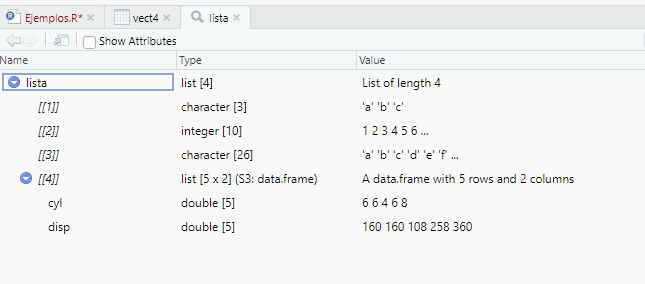
\includegraphics[keepaspectratio]{imagenes/05listas.png}}

}

\caption{Si queremos llamar un objeto dentro de una lista simplemente
escribimos el nombre de la lista abrimos doble corchete y ponemos dentro
el numero de orden que corresponde el elemento que queremos,}

\end{figure}%

\begin{Shaded}
\begin{Highlighting}[]
\NormalTok{lista[[}\DecValTok{1}\NormalTok{]] }\CommentTok{\#nos nos arroja el resultado de todo el contenido del elemento 1, que en este caso es un vector}
\end{Highlighting}
\end{Shaded}

\begin{verbatim}
[1] "a" "b" "c"
\end{verbatim}

Dentro de los ejercicios que vamos a hacer usaremos las listas, por
ejemplo, con estas podemos cargar múltiples archivos como objetos desde
una carpeta para facilitar el proceso de importación.

Aquí un escenario de ejemplo:

En la carpeta de \textbf{``datos''} o ``\textbf{Fuente''} dentro del
proyecto en que se esté trabajando digamos que hay 3 bases de datos en
formato excel con similar estructura (ejemplo, provincia\_a.xlsx,
provincia\_b.xlsx, provincia\_c.xlsx) y la tarea es unir estas bases de
datos en una sola base de datos:

\begin{Shaded}
\begin{Highlighting}[]
\CommentTok{\#Cargando el paquete \{rio\} para importar bases de datos y \{tidyverse\} para manipulación de datos}
\NormalTok{pacman}\SpecialCharTok{::}\FunctionTok{p\_load}\NormalTok{(rio,      }
\NormalTok{               tidyverse)  }

\CommentTok{\#para crear un vector con las rutas completa de varios archivos}
\NormalTok{ruta\_archivos }\OtherTok{\textless{}{-}} \FunctionTok{dir}\NormalTok{(}\StringTok{"datos"}\NormalTok{, }\CommentTok{\#nombre de la carpeta donde están los archivos fuente}
                     \AttributeTok{pattern =} \StringTok{"xlsx"}\NormalTok{, }\CommentTok{\#patrón presente en todos los archivos a importar}
                     \AttributeTok{full.names =} \ConstantTok{TRUE} \CommentTok{\#argumento para crear la ruta completa de cada archivo}
\NormalTok{                     )}

\NormalTok{lista\_bases }\OtherTok{\textless{}{-}} \FunctionTok{map}\NormalTok{(ruta\_archivos, import)}\CommentTok{\# la funcion map (que viene de tidyiverse) va a crear un objeto lista que va a contener cada una de las bases de datos que fueron especificadas en el vector ruta\_archivos}

\FunctionTok{head}\NormalTok{(lista\_bases[[}\DecValTok{1}\NormalTok{]]) }\CommentTok{\#este comando nos permite ver las primeras 5 filas en la base de datos localizada en la posición 1}
\end{Highlighting}
\end{Shaded}

\section{Funciones}\label{funciones}

Otro tipo de objeto que no necesariamente almacena datos, pero sí
podemos crear objetos de datos, son las funciones. Si te has dado
cuenta, hasta ahora se han mencionado mucho dado que todo el código que
vamos a ir escribiendo se hace mayormente con funciones, de hecho, como
se mencionó arriba, la mayoría de los paquetes son una compilación de
funciones. Nosotros podemos crear funciones que usan funciones ya sean
de R base o incluso de otros paquetes.

Las funciones nos ayudan a agilizar el trabajo porque son un conjunto de
instrucciones dentro de nuestra rutina. Un ejemplo de esto es que
podemos crear una función que nos produzca un gráfico de curva epidémica
de un período y lugar determinados y obtendríamos el resultado, el
gráfico, y los dos parámetros: el periodo y el lugar.

Para crear una función usamos la siguiente sintaxis:

\pandocbounded{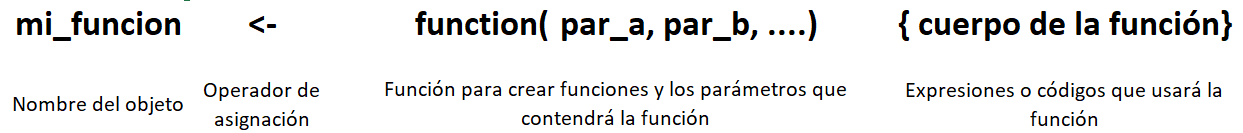
\includegraphics[keepaspectratio]{imagenes/05funcion.png}}

Vamos hacer un ejercicio simple para entender mejor una función:

\begin{Shaded}
\begin{Highlighting}[]
\CommentTok{\#una funcion para calcular el indice de masa corporal}
\NormalTok{mi\_funcion }\OtherTok{\textless{}{-}} \ControlFlowTok{function}\NormalTok{(peso, altura)\{ }
  
\NormalTok{  resultado }\OtherTok{\textless{}{-}} \FunctionTok{round}\NormalTok{(peso}\SpecialCharTok{/}\NormalTok{(altura}\SpecialCharTok{/}\DecValTok{100}\NormalTok{)}\SpecialCharTok{\^{}}\DecValTok{2}\NormalTok{,}\DecValTok{2}\NormalTok{) }\CommentTok{\#asigna al elemento resultado el la operación entre peso y altura y luego redondear el valor}
  
  \FunctionTok{print}\NormalTok{(}\FunctionTok{paste0}\NormalTok{(}\StringTok{"Formula: "}\NormalTok{,peso,}\StringTok{"kg./"}\NormalTok{,altura}\SpecialCharTok{/}\DecValTok{100}\NormalTok{,}\StringTok{"(m)2"}\NormalTok{)) }\CommentTok{\# retorna un texto con el peso y la altura}
  
  \FunctionTok{print}\NormalTok{(}\FunctionTok{paste0}\NormalTok{(}\StringTok{"El indice de masa corporal es "}\NormalTok{, resultado)) }\CommentTok{\# retorna el en un solo texto el indice de masa corporal obtenido}
  
\NormalTok{\}}

\FunctionTok{mi\_funcion}\NormalTok{(}\AttributeTok{peso=}\DecValTok{115}\NormalTok{,}\AttributeTok{altura=}\DecValTok{180}\NormalTok{) }\CommentTok{\#llamamos la funcion y escribimos los parametros}
\end{Highlighting}
\end{Shaded}

\begin{verbatim}
[1] "Formula: 115kg./1.8(m)2"
[1] "El indice de masa corporal es 35.49"
\end{verbatim}

Para entender mejor cómo trabaja una función usando el ejemplo anterior,
escribimos la función \textbf{function()\{ \}} luego del nombre de la
función y el operador de asignación, y dentro de los paréntesis
escribimos el nombre que queremos usar para los parámetros separados por
coma, como hicimos en el ejemplo anterior, usamos peso y altura. Luego,
dentro de las llaves vamos a proceder a escribir las expresiones para
obtener un resultado; para esta función que calcula el índice de masa
corporal (IMC), creamos un vector que es el resultado de la operación de
la fórmula del IMC, donde el parámetro 1 es el peso que es dividido
entre el parámetro 2, luego el parámetro 2 que es la altura, que a su
vez es dividida entre 100 y luego elevada al cuadrado; la siguiente
expresión presenta un texto con los parámetros y luego presenta otro
texto con el resultado del IMC.

De las funciones se pueden escribir libros, de hecho, hay una vasta
documentación de cómo trabajar con ellas, pues son el pilar de la
programación en R.

Cuando te sientas más familiarizado y tengas más experiencia en R,
puedes dedicarle tiempo a aprender sobre cómo trabajar más profundamente
con las funciones. Por ahora, vamos a enfocarnos en los paquetes, que
tienen funciones que nos facilitan el trabajo para el análisis de datos.

\bookmarksetup{startatroot}

\chapter{Transición desde Excel a
R}\label{transiciuxf3n-desde-excel-a-r}

En el aprendizaje de hacer análisis de datos usualmente se comienza
usado hojas de cálculo como Microsoft Excel® para hacer tareas comunes
como tablas, gráficos y cálculos estadísticos de forma general.

Si ya estás trabajando con datos de forma regular, es muy probable que
también te hayas expuesto a Excel, o lo usas constantemente en tu día a
día como parte de las herramientas para procesar, analizar y presentar
datos.

En nuestro caso, incluso sabiendo de la existencia de R, creíamos que
con Excel podíamos hacerlo todo, como resolver cualquier situación
relacionada con los datos, dado que MS Excel tiene muchas
funcionalidades y es una herramienta muy completa como hoja de cálculo.

A pesar de lo robusto que puede ser Excel u otra hoja de cálculo, hay
límites donde la funcionalidad de R va más allá, empezando por la
cantidad de datos que se pueden cargar en un archivo de Excel, el cual
tiene un límite de 1,048,576 filas por hoja y 16,384 columnas, y aunque
se puede usar Power Query para tener más filas y columnas, no menos
cierto es que el archivo se hace muy ``pesado'' o ``lento'' para
trabajar cuando se usa cierta cantidad de filas y/o columnas. Con R se
pueden manejar bases de datos más grandes de manera más rápida,
dependiendo de la memoria RAM instalada de la computadora. Te
recomendamos que busques en la web cómo aumentar la memoria RAM de tu
computadora.

Volviendo a Excel, una hoja de cálculo en general es muy intuitiva y
fácil de aprender, solo con abrir una hoja podemos comenzar a escribir
agregando datos, escribir funciones para cálculos, hacer gráficos, etc.,
todo en un entorno guiado a través de los clics del ratón.

En cambio, R, como es un lenguaje de programación, es basado en
comandos, sintaxis, donde mayormente todo debe de ser escrito, y
realmente, es poco intuitivo al momento de comenzar a usarlo debido a lo
complejo que resulta aprender un lenguaje nuevo. Sin embargo, esta forma
de proceder a través de texto, también tiene sus ventajas cuando vamos a
realizar una tarea, dado que debemos tener definido, de una forma u
otra, lo que vamos a hacer y cuáles comandos deben de ser ejecutados
para lograr la tarea. De hecho, de forma general, así es que debemos de
trabajar, es decir, primero tener un plan en mente, cómo será ejecutado
y definir cada paso. La idea es que el cambio de ambiente (pasar de usar
más el ratón que escribir) puede ser un poco difícil al principio y
sentirnos frustrados, pero con la constante exposición a un nuevo
ambiente nos vamos adaptando, y se le hace fácil al cerebro en la medida
que vamos practicando cada vez más y más.

En pocas palabras, es estar un poco ``abierto'' a cosas nuevas y darse
la oportunidad de aprender y esforzarse más.

\section{Tareas que se realizan en Excel (u otras hojas de cálculos) y
su equivalente en
R}\label{tareas-que-se-realizan-en-excel-u-otras-hojas-de-cuxe1lculos-y-su-equivalente-en-r}

Entrando en el tema de que cosas podemos hacer muy parecidas en R que se
hacen con Excel, que son muy propias de lo que hacemos en epidemiología
cuando analizamos datos es la exploración, en R podemos al igual que
Excel podemos ver las bases de datos en un formato muy parecido a Excel,
por ejemplo, podemos usar el comando \textbf{\emph{View()}} (con V
mayúscula) puedes escribir en la consola
\textbf{\emph{View(mtcars)\hyperref[_ftn1]{{[}1{]}}}} y se nos abrirá
una ventana una tabla (no editable por cierto) pero nos sirve para ver
los datos y filtrar muy parecido a Excel.

Otra tarea muy común que realizamos en Excel son las ``pivot tables'' o
tablas dinámicas, que nos permiten hacer tablas resúmenes de una base de
datos con unos cuantos clics de ratón, en R, podemos hacer lo mismo con
varios comandos.

\begin{figure}[H]

{\centering \pandocbounded{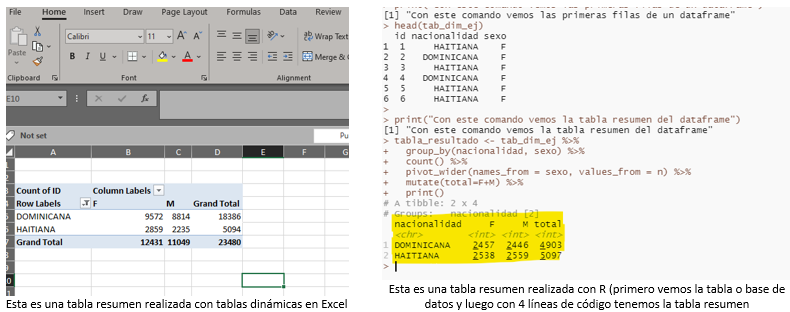
\includegraphics[keepaspectratio]{imagenes/06pivottables.png}}

}

\caption{Comparación entre Excel y R, tablas dinámicas}

\end{figure}%

A simple vista se pudiera ver que en R es más complicado porque hay que
escribir lo que se va a realizar, pero tomando en cuenta que en nuestro
trabajo del día a día como investigadores hacemos muchas tablas
resúmenes en Excel o tenemos que actualizarlas, y esto realmente toma
mucho tiempo, sin embargo, en R solo nos tome tiempo hacer la primera
tabla resumen, y posteriormente, tendríamos la ventaja de reusar el
código solo cambiando algunos parámetros (como las variables),
ahorrándonos mucho tiempo al no tener que repetir la misma tarea una y
otra vez.

En Excel también usamos mucho las funciones y fórmulas para hacer
cálculos, un ejemplo común es crear grupos de edades a partir de una
variable numérica que representa la edad. De una forma u otra, usar
funciones o fórmulas en Excel es similar a escribir códigos, y si puedes
hacer fórmulas en Excel, entonces significa que ¡ya tienes experiencia
codificando! En R, gracias a la disponibilidad de tantos paquetes (como
el~\textbf{epikit}), tenemos funciones que son específicamente para esto
que se requiere menos esfuerzo.

En resumen, hay una vasta documentación disponible sobre cómo adaptarse
al uso de R para usuarios de Excel, cuáles son las diferencias entre R y
Excel y cómo se complementan. Cuando veamos sobre exportación de datos,
veremos un buen ejemplo de esto.

En la web hay mucha documentación acerca de cómo acostumbrarse a
realizar análisis de datos con R para usuarios de otros programas;
recomendamos que hagas una búsqueda sobre el tema para que vayas
adaptándote.

Nuestra mayor recomendación es que comiences a practicar con R haciendo
lo que ya sabes hacer con Excel. También puedes fácilmente ver la
documentación de una función ecribiendo el signo de interrogración
(\textbf{?}) delante de la función que quieres:~\textbf{?sum()}~y luego
en el panel de ayuda vas a ver cuáles son los argumentos y también un
ejemplo. En caso de no entender, busca en internet. ¿Te has dado cuenta
de que hacemos mucho enfasís en~\textbf{\emph{``Buscar en la web''}}? Es
porque esa es la mayor ventaja que tiene R como lenguaje de programación
para análisis de datos, la comunidad de apoyo.

\hyperref[_ftnref1]{{[}1{]}} mtcars es una base de datos que trae R
internamente como ejemplo sobre carros, para saber más de esta escribe
en la consola help(``mtcars'')\footnote{\textbf{mtcars} es una base de
  datos que trae R internamente como ejemplo sobre carros, para saber
  más de esta escribe en la consola help(``mtcars'')}

\bookmarksetup{startatroot}

\chapter{Análisis de datos usando
R}\label{anuxe1lisis-de-datos-usando-r}

\section{Tareas que se deben de hacer para llevar a cabo un proyecto de
análisis de
datos}\label{tareas-que-se-deben-de-hacer-para-llevar-a-cabo-un-proyecto-de-anuxe1lisis-de-datos}

Es posible que ya tengas conocimiento sobre la estructura del documento
que debes desarrollar para analizar tus datos, ya sea para toma de
decisiones o para elaborar un trabajo final. En esta sección nos
enfocaremos en la generación de resultados o salidas de R, donde tienes
que realizar tablas, gráficos y análisis estadísticos. A continuación,
te mostramos un listado de los elementos requeridos en la sección de
resultados partiendo de un contexto clínico o epidemiológico:

\begin{itemize}
\item
  Proporciona número de casos, incidencia o prevalencia de un evento.
\item
  Características clínicas, por ejemplo, síntomas comunes, porcentaje de
  hospitalizados o fallecidos, resultados de laboratorio como porcentaje
  de confirmados o distribución por especie o subtipo (generalmente
  presentados en una tabla).
\item
  Tiempo: casos por año, mes, semana u otro intervalo apropiado, para
  mostrar patrones o cambios a lo largo de un período determinado. Puede
  estratificarse por grupos de edad, sexo, región o características de
  persona; lugar (generalmente se presenta en un gráfico). Señale
  cambios importantes, tendencias estacionales, aberraciones (Ej.,
  Brotes) u otros patrones inusuales.
\item
  Lugar: como el área geográfica donde ocurre el evento. Esto,
  generalmente, se presenta con un mapa o una tabla.
\item
  Persona, por ejemplo, por grupo de edad, sexo y otras características
  relevantes (generalmente presentadas en una tabla).
\end{itemize}

Existen otros resultados destacados que no se incluyen en las categorías
enumeradas anteriormente. Por ejemplo, muchos informes resumidos de
vigilancia epidemiológica incluyen datos sobre la integridad y
puntualidad de los informes de cada fuente de informes.

Con una base de datos de ejemplo vamos a realizar los pasos en R para
producir los requerimientos sugeridos anteriormente. Vamos a usar como
fuente de datos para este ejercicio una base de datos de casos de VIH
positivos notificados. (Esta base está disponible en el siguiente
\textbf{link}).

Esta base de datos (o la que vayas a usar) debes de colocarla en la
subcarpeta de \textbf{``Bases de datos''} dentro de la carpeta del
\textbf{proyecto} (ejemplo la mi carpeta donde está el proyecto de
Rstudio se llama trabajos de campo)\textbf{.} A modo de refrescamiento,
ver la siguiente imagen de la estructura de sub-carpetas de un proyecto,
su jerarquía.

\begin{figure}[H]

{\centering \pandocbounded{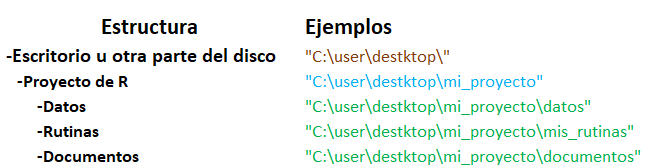
\includegraphics[keepaspectratio]{imagenes/07estructuraex.png}}

}

\caption{Estructura básica recomendada para un proyecto en rstudio.}

\end{figure}%

\subsection{Organización general antes de
comenzar}\label{organizaciuxf3n-general-antes-de-comenzar}

Como refrescamiento, antes de comenzar recuerda crear el proyecto (ver
la sección de Comenzar a trabajar con R y la interfaz de Rstudio)

\textbf{Procesamiento de datos (cargar, editar, transformar
\emph{dataframes})}

\begin{itemize}
\item
  Crear un documento de rutina de R, (Ctrl+shift+N o en File, R script),
\item
  Comentar al menos el título del trabajo que estas haciendo (escribir
  \# , que es el carácter para hacer comentarios, después de este puedes
  escribir cualquier cosa y no será interpretado como código).
\item
  Instalar el paquete
  \href{http://trinker.github.io/pacman/vignettes/Introduction_to_pacman.html}{\textbf{pacman}}(luego
  nos permitirá con mayor facilidad instalar el resto)
\item
  Cargar los siguientes paquetes:
\end{itemize}

\begin{enumerate}
\def\labelenumi{\arabic{enumi}.}
\item
  \href{https://cran.r-project.org/web/packages/rio/vignettes/rio.html}{\textbf{rio}}
  (para cargar archivos excel y otros formatos)
\item
  \href{https://cran.r-project.org/web/packages/tidyverse/vignettes/paper.html}{\textbf{tidyverse}}
  (para transformar, revisar la base de datos)
\item
  \href{https://cran.r-project.org/web/packages/janitor/vignettes/janitor.html}{\textbf{janitor}}
  (para tablas y limpieza de datos)
\item
  \href{https://cran.r-project.org/web/packages/flextable/index.html}{\textbf{flextable}}
  (para formato de presentación de las tablas)
\item
  \href{https://cran.r-project.org/web/packages/lubridate/vignettes/lubridate.html}{\textbf{lubridate}}
  (para trabajar con funciones con variables de formatos de fecha)
\item
  \href{https://cran.r-project.org/web/packages/skimr/vignettes/skimr.html}{\textbf{skimr}}
  (para revisar la base de datos)
\item
  \href{https://cran.r-project.org/web/packages/here/vignettes/here.html}{\textbf{here}}
  (para ayudarnos a encontrar los archivos que vamos a usar, también a
  guardarlos)
\item
  \href{https://www.danieldsjoberg.com/gtsummary/}{\textbf{gtsummary}}
  (para hacer tablas presentables y cálculos que usamos con frecuencia
  en epidemiología)
\end{enumerate}

Para cargar estos paquetes procedemos a usar la función
\textbf{p\_load()} del paquete \emph{\{pacman\}}, en el panel de editor
de rutinas, escribes el siguiente comando:

\begin{Shaded}
\begin{Highlighting}[]
\FunctionTok{install.packages}\NormalTok{(}\StringTok{"pacman"}\NormalTok{) }\CommentTok{\#para instalar el paquete pacman (solo una vez)}
\end{Highlighting}
\end{Shaded}

\begin{Shaded}
\begin{Highlighting}[]
\NormalTok{pacman}\SpecialCharTok{::}\FunctionTok{p\_load}\NormalTok{(rio, }
\NormalTok{               tidyverse, }
\NormalTok{               janitor, }
\NormalTok{               lubridate, }
\NormalTok{               skimr, }
\NormalTok{               here,}
\NormalTok{               flextable,}
\NormalTok{               gtsummary) }\CommentTok{\#para instalar y cargar los paquetes necesarios}
\end{Highlighting}
\end{Shaded}

Luego de copiar o de introducir el código, preciona \textbf{Ctrl+ENTER}
al final de la línea de código o en ``run'' para ejecutarlo.

Otra alternativa para cargar los paquetes es con la función de R base
\textbf{library()}. Al igual que con p\_load() de pacman, escribes el
nombre o los nombres de los paquetes separados por coma. \textbf{Ojo,}
esta función solo carga los paquetes, si el paquete no está instalado,
te dará error.

NOTA: Debes tener conexión a internet para poder descargar estos
paquetes.

Después de instalar los paquetes no necesitarás instalarlos de nuevo, a
menos que re-instales o actualices Rstudio.

Antes de continuar, guarda la rutina en la carpeta de tu proyecto
``rutinas'' utilizando cualquiera de estas opciones:

\begin{itemize}
\item
  Presionando la combinación de teclas \textbf{Ctrl+S}
\item
  Haciendo clic en el icono de guardar
\item
  Desde el menú: File -\textgreater{} Save
\end{itemize}

El próximo paso es cargar la base de datos, y esto lo podemos hacer de
dos formas: escribiendo directamente en la rutina o en la consola, tal
como vimos cuando explicamos los \textbf{dataframes} en el capítulo 5 de
objetos de R, o bien, usando la interfaz de Rstudio.

Recuerda tener tus bases de datos en la carpeta de ``datos'' dentro de
tu carpeta del proyecto, esto es muy importante para facilitar el
trabajo.

Vamos a ver cómo sería el código para cargar un archivo de Excel:

\begin{Shaded}
\begin{Highlighting}[]
\CommentTok{\#para crear un objeto dataframe (nuestra base)}
\NormalTok{base }\OtherTok{\textless{}{-}} \FunctionTok{import}\NormalTok{(}\FunctionTok{here}\NormalTok{(}\StringTok{"datos"}\NormalTok{, }\StringTok{"sinave\_vih.xlsx"}\NormalTok{)) }\SpecialCharTok{\%\textgreater{}\%} 
         \FunctionTok{clean\_names}\NormalTok{()}
\end{Highlighting}
\end{Shaded}

Explicando un poco el código anterior: estamos creando un nuevo objeto
llamado \textbf{``base'',}a través de la función de \textbf{import} del
paquete \textbf{rio}, que sirve para cargar archivos tipo .xls, .xlsx.,
y con la finalidad de localizar la ruta del archivo de la forma más
sencilla posible, usamos la función \textbf{here()} del paquete
\textbf{here} escribiendo los parámetros de la sub-carpeta, es decir,
agregando entre comillas el nombre de la carpeta donde está la base de
datos (primer parámetro: ``datos), y después de una coma se agrega el
segundo parámetro que es el nombre del archivo, en este ejemplo, el
archivo se denomina \emph{sinave\_vih.xlsx}. Luego sigue un operador
pipe (\%\textgreater\%) que significa ``luego'' y a través de la función
\textbf{clean\_names()} del paquete \textbf{janitor} podremos
``normalizar'' los nombres de las columnas o variables de la base de
datos importada. Esta normalización consiste, por ejemplo, en
estandarizar los nombres de las variables poniéndolas todas en
minúsculas, quitar caracteres poco comunes o espacios, entre otros
ajustes que consideremos importantes.

Si estás utilizando la misma base de datos del ejemplo, y si hiciste los
pasos correctamente, debes de tener una imagen similar a la de la Figura
23, donde puedes ver a la derecha que ya tienes un objeto
\emph{dataframe} cargado (es decir, la base de datos) que contiene
25,227 filas y 71 variables o columnas. (ver figura
Figura~\ref{fig-bdimportada})

\begin{figure}

\centering{

\pandocbounded{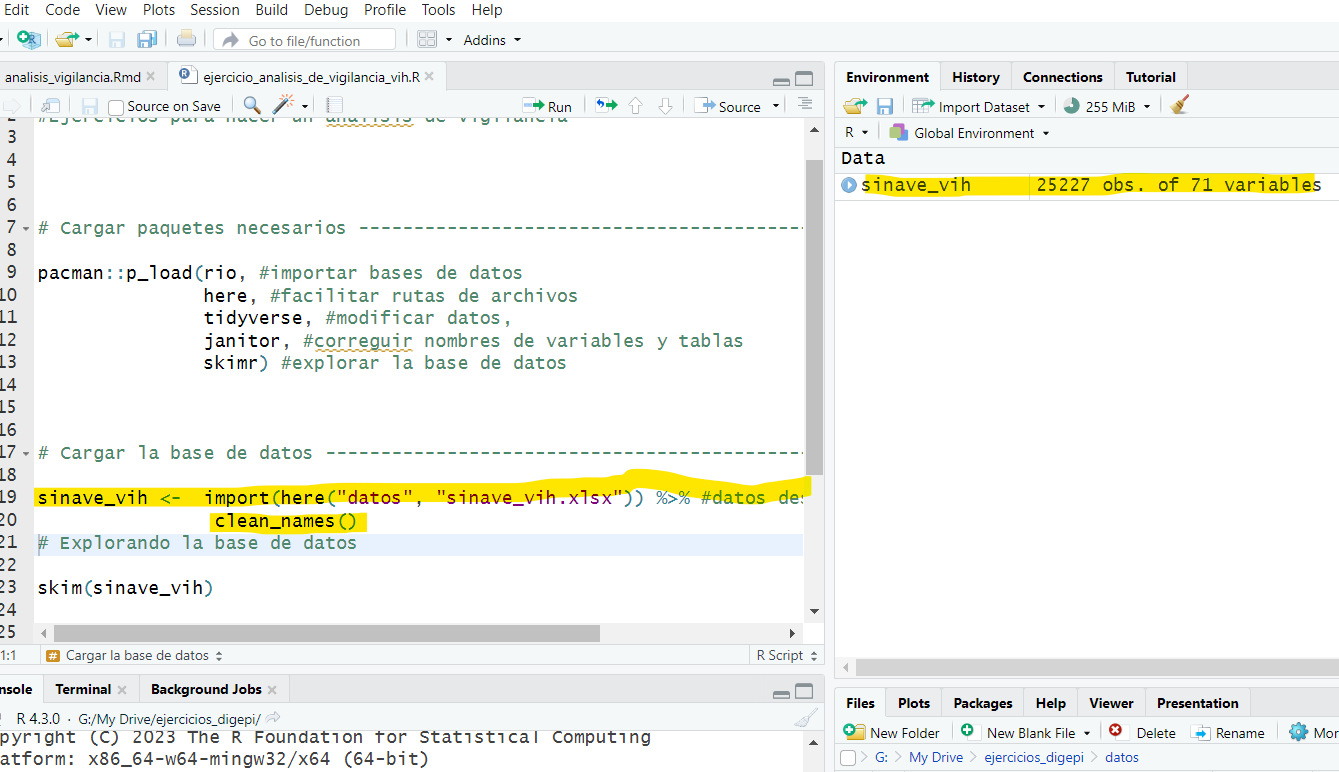
\includegraphics[keepaspectratio]{imagenes/07cargarbase.png}}

}

\caption{\label{fig-bdimportada}}

\end{figure}%

Donde puedes ver a la derecha que ya tienes un objeto dataframe cargado
(la base de datos) que tiene 25,227 filas y 71 variables o columnas.

\subsubsection{\texorpdfstring{\textbf{Exploración de la base de
datos}}{Exploración de la base de datos}}\label{exploraciuxf3n-de-la-base-de-datos}

Entonces, la primera pregunta que te hacemos es; ¿Cuál es el próximo
paso por seguir? Realmente debería ser el análisis, pero primero, sería
bueno revisar la base de datos para ver los datos ``malos'' es decir,
hacer una exploración para identificar valores anormales, campos vacíos
o datos que se cargaron mal, como pasa a veces con las fechas.

El paquete de \{\textbf{rio\}} con la fórmula de \textbf{import()} hace
un intento de determinar los tipos de variables que se cargan desde el
archivo de Excel, pero a veces falla y es, usualmente, con las fechas,
porque sin querer había una fecha escrita en un formato no reconocido y
el resto como número.

Para explorar la base de datos, podemos hacerlo de forma directa
haciendo clic en el panel de ambiente de trabajo en el objeto base (o el
nombre que le hayas dado), o puedes escribir en la consola de comandos
\textbf{View(base)} para cargar el visor de datos.

Otra forma más completa de explorar la base de datos es a través de la
función \textbf{skim()} o \textbf{skim\_tee()} del paquete
\{\textbf{skimr\}} (Waring et al. 2022), puedes utilizar cualquiera de
las dos porque ambas producen el mismo reporte. Con estas funciones
obtendremos un resumen de cada variable, qué tipo de variable es cada
una y muestra el total de campos vacíos, valores únicos, entre otros
detalles importantes.

Con estos simples pasos, ya estamos entrando de lleno en el análisis.
Recuerda, siempre el primer paso es verificar los datos, si hay valores
extremos, datos faltantes, etc., esta es una buena práctica (diríamos
que obligatoria) cuando estamos haciendo análisis, luego viene la
limpieza de los datos.

Luego de escribir en tu rutina el último comando, debes tener escrito el
siguiente código y obtener este resultado:

\begin{Shaded}
\begin{Highlighting}[]
\NormalTok{base }\OtherTok{\textless{}{-}} \FunctionTok{import}\NormalTok{(}\FunctionTok{here}\NormalTok{(}\StringTok{"datos"}\NormalTok{, }\StringTok{"sinave\_vih.xlsx"}\NormalTok{)) }\SpecialCharTok{\%\textgreater{}\%} 
  \FunctionTok{clean\_names}\NormalTok{()}

\NormalTok{skimr}\SpecialCharTok{::}\FunctionTok{skim\_tee}\NormalTok{(base) }\CommentTok{\#para genera un mini reporte de la base}
\end{Highlighting}
\end{Shaded}

\begin{verbatim}
-- Data Summary ------------------------
                           Values
Name                       data  
Number of rows             25615 
Number of columns          41    
_______________________          
Column type frequency:           
  character                20    
  logical                  1     
  numeric                  17    
  POSIXct                  3     
________________________         
Group variables            None  

-- Variable type: character ----------------------------------------------------
   skim_variable           n_missing complete_rate min max empty n_unique
 1 sexo                            0       1         8   9     0        2
 2 grupo_edad                      0       1         2   8     0        9
 3 actividad_ocupacional       24767       0.0331    5 120     0      167
 4 grupo_ocupacional           24769       0.0330   21  76     0       10
 5 categoria_de_afiliacion         0       1        10  23     0        5
 6 nivel_educativo              6763       0.736     8  25     0        6
 7 provincia                       0       1         2   2     0       33
 8 colectivo                    8976       0.650     6  36     0       11
 9 region                          0       1         1   4     0        9
10 tipo_atencion                  82       0.997     8  13     0        4
11 complicaciones              24005       0.0629    7  69     0       19
12 muestra                       268       0.990     2   2     0        2
13 resultado_final             20575       0.197     9  10     0        3
14 condicion                       0       1         4   6     0        2
15 gravedad                    16183       0.368     5  20     0        3
16 edad_fecha_defuncion        25510       0.00410   5   8     0       74
17 diag_final                  24394       0.0477   10  56     0        6
18 clasf_final                 24394       0.0477   10  10     0        3
19 fuente_deteccion                0       1        14  24     0        5
20 confirmado_por              24396       0.0476   11  19     0        2
   whitespace
 1          0
 2          0
 3          0
 4          0
 5          0
 6          0
 7          0
 8          0
 9          0
10          0
11          0
12          0
13          0
14          0
15          0
16          0
17          0
18          0
19          0
20          0

-- Variable type: logical ------------------------------------------------------
  skim_variable         n_missing complete_rate mean count
1 fecha_inicio_erupcion     25615             0  NaN ": " 

-- Variable type: numeric ------------------------------------------------------
   skim_variable          n_missing complete_rate       mean       sd    p0
 1 pxid                           0         1     12808      7395.        1
 2 fecha_nacimiento               0         1     30282.     4960.     8416
 3 edad1                        119         0.995    36.8      13.4       0
 4 edad2                      20494         0.200     0.0842    0.710     0
 5 edad3                      20537         0.198     0.101     1.40      0
 6 pais_procedencia               0         1         1.18      0.398     1
 7 semana_inicio_sintomas         0         1        25.6      15.3       1
 8 mes_inicio_sintomas            0         1         6.32      3.50      1
 9 ano_inicio_sintomas            0         1      2019.        1.41   2016
10 semana_atencion                0         1        25.7      15.2       1
11 mes_atencion                   0         1         6.31      3.48      1
12 ano_atencion                   0         1      2019.        1.40   2017
13 semana_toma_muestra        13577         0.470    25.5      14.9       1
14 fecha_toma_muestra         13577         0.470 43672.      531.    42737
15 institucion                    0         1         4.53      0.757     1
16 semana_notificacion            0         1        26.1      15.0       1
17 fecha_notificacion             0         1     43738.      513.    42738
      p25   p50    p75  p100 hist 
 1  6404. 12808 19212. 25615 ▇▇▇▇▇
 2 27144. 30902 33921  44501 ▁▁▆▇▁
 3    27     35    45     98 ▁▇▅▁▁
 4     0      0     0     11 ▇▁▁▁▁
 5     0      0     0     30 ▇▁▁▁▁
 6     1      1     1      3 ▇▁▂▁▁
 7    11     26    39     53 ▇▆▇▆▆
 8     3      6     9     12 ▇▅▅▅▇
 9  2018   2019  2020   2021 ▆▆▇▆▇
10    11     26    39     53 ▇▆▆▆▆
11     3      6     9     12 ▇▅▅▅▇
12  2018   2019  2020   2021 ▅▆▇▆▇
13    12     25    38     53 ▇▆▆▆▆
14 43214  43638 44174  44567 ▆▆▇▅▇
15     4      5     5      5 ▁▁▂▂▇
16    12     26    39     53 ▇▆▇▆▆
17 43315  43718 44232  44615 ▅▆▇▆▇

-- Variable type: POSIXct ------------------------------------------------------
  skim_variable         n_missing complete_rate min                
1 fecha_inicio_sintomas         0       1       2016-12-03 00:00:00
2 fecha_atencion                0       1       2017-01-02 00:00:00
3 fecha_defuncion           25510       0.00410 2017-02-03 00:00:00
  max                 median              n_unique
1 2022-01-01 00:00:00 2019-08-15 00:00:00     1811
2 2022-01-01 00:00:00 2019-08-23 00:00:00     1653
3 2022-01-01 00:00:00 2020-10-06 00:00:00      100
\end{verbatim}

En el ejemplo anterior:

\begin{itemize}
\item
  ¿Cuántas variables de texto, numéricas, lógicas (si/no, 1/0), de
  fechas se cargaron?
\item
  ¿Cuantas de las variables están en blanco o tienen muchos valores
  vacíos, cómo es la distribución de las variables numéricas y fechas,
  (valores extremos)?
\item
  ¿Hay variables que se importaron incorrectamente? Variables que son de
  un formato y se importaron de otro tipo (fechas que se importan como
  texto o número por ejemplo)
\end{itemize}

Estas son las preguntas que debemos hacernos a partir de este resumen,
para ir viendo la data y hacer la limpieza de datos, excluir columnas o
variables, filtrar valores extremos o editarlos, cambiar o corregir el
formato, etc.

En el ejemplo anterior vemos que vemos que el resultado arrojó 4 tablas
con un tipo de variable cada una. La reproducimos aquí para visualizarla
mejor:

\pandocbounded{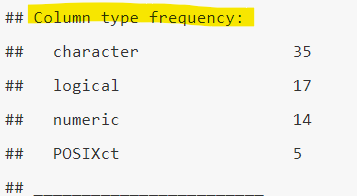
\includegraphics[keepaspectratio]{imagenes/07skimr2.png}}

Debajo de ``\emph{Column type frequency}'' veremos en detalle cuatro
tablas consecutivas, una conteniendo las variables de tipo ``caracter'',
la que sigue muestra las variables de tipo ``lógico'', y así
sucesivamente. Puedes notar el detalle dentro de cada tabla donde se
indica el nombre de cada variable, el total de campos vacíos, la tasa de
completitud, valores mínimos, máximos, promedios y valores únicos. Este
resultado ofrece un resumen que nos facilita la exploración rápida de la
base de datos.

A continuación, podemos ver resaltado los detalles que la función skim()
nos brinda, como es un inventario de las variables de un dataframe por
tipo de variable.

\pandocbounded{\includegraphics[keepaspectratio]{.pdf}}

\begin{figure}[H]

{\centering \pandocbounded{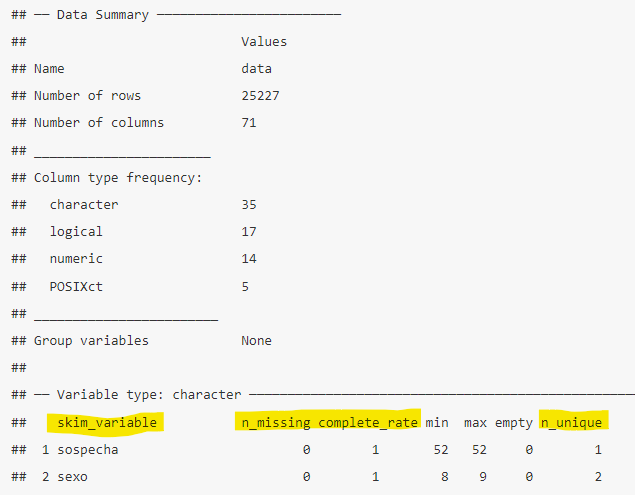
\includegraphics[keepaspectratio]{imagenes/07skimr.png}}

}

\caption{Resaltado podemos ver los detalles que la función skim() nos
brinda como es un inventario de las variables de un dataframe por tipo
de variable.}

\end{figure}%

En general, después de este resumen se pueden definir los próximos pasos
para el análisis, incluso lo puedes incluir en tu reporte como anexo
para añadir más ``confianza'' a tus hallazgos y conclusiones, porque
estás mostrando de forma rápida la ``salud'' de tus datos.

Esta exploración inicial puedes hacerla de diferentes maneras, sin
embargo, usar el paquete \textbf{skimr} es la manera más amigable,
detallada y rápida.

A medida que vamos avanzando con este ejercicio, explicararemos con más
detalles los tipos de campos y variables que identifica R.

\subsubsection{Limpieza /re-structuración de
datos}\label{limpieza-re-structuraciuxf3n-de-datos}

En este paso vamos a modificar la base de datos para prepararla antes de
iniciar con nuestro análisis. Tomando en cuenta que debes de preparar un
plan de análisis y que este se enfocará en un análisis tipo descriptivo
(en tiempo, lugar y persona), vamos a ejecutar los siguientes pasos:

\begin{itemize}
\item
  Vamos a revisar el listado de variables que obtuvimos del resumen del
  ejercicio anterior para seleccionar las que necesitamos para el
  análisis.
\item
  Vamos a re-codificar variables que necesiten cambios o ajustes.
\item
  Vamos a excluir o modificar los valores de las variables de interés.
\end{itemize}

Una de las características poderosas y deseadas de R es que puedes crear
un nuevo objeto a partir de otro, dado que puedes hacer múltiples
versiones del original.

Para este análisis vamos a crear un nuevo objeto dataframe que podemos
llamar base\_arreglada, en la que solo tendremos las variables o
columnas que necesitaremos para nuestro análisis, y trataremos de
excluir los valores no deseados creando nuevas variables a partir de las
que ya tenemos.

Agrega a tu rutina el siguiente código:

\begin{Shaded}
\begin{Highlighting}[]
\NormalTok{base\_arreglada }\OtherTok{\textless{}{-}}\NormalTok{ base }\SpecialCharTok{\%\textgreater{}\%} \CommentTok{\#creamos un nuevo elemento}

  \FunctionTok{select}\NormalTok{(fecha\_notificacion, }\CommentTok{\#seleccionamos las variables que necesitamos}
\NormalTok{         fecha\_atencion,}
\NormalTok{         mes\_atencion,}
\NormalTok{         ano\_atencion,}
\NormalTok{         semana\_atencion,}
\NormalTok{         sexo,}
\NormalTok{         pais\_procedencia,}
\NormalTok{         grupo\_edad,}
\NormalTok{         edad1,}
\NormalTok{         nivel\_educativo,}
\NormalTok{         provincia,}
\NormalTok{         clasf\_final,}
\NormalTok{         condicion) }\SpecialCharTok{\%\textgreater{}\%} 
  
  \FunctionTok{filter}\NormalTok{(}\SpecialCharTok{!}\FunctionTok{is.na}\NormalTok{(edad1)) }\SpecialCharTok{\%\textgreater{}\%}  \CommentTok{\#filtramos aquellos casos que no tienen edad}
  
  \FunctionTok{mutate}\NormalTok{(}\AttributeTok{fecha\_notificacion=}\FunctionTok{excel\_numeric\_to\_date}\NormalTok{(fecha\_notificacion), }\CommentTok{\#corrige el formato de la fecha (de numero a fecha),}
   \AttributeTok{prov\_recla =} \FunctionTok{case\_when}\NormalTok{(provincia}\SpecialCharTok{==}\StringTok{"01"} \SpecialCharTok{|}\NormalTok{ provincia}\SpecialCharTok{==}\StringTok{"02"}\SpecialCharTok{\textasciitilde{}}\StringTok{"provincia capital"}\NormalTok{,}
                          \ConstantTok{TRUE}\SpecialCharTok{\textasciitilde{}}\NormalTok{provincia)) }\SpecialCharTok{\%\textgreater{}\%} 
  \FunctionTok{distinct}\NormalTok{() }\CommentTok{\#para remover filas duplicadas}
  
  \FunctionTok{head}\NormalTok{(base\_arreglada) }\CommentTok{\#para ver un ejemplo de la nueva base}
\end{Highlighting}
\end{Shaded}

\begin{verbatim}
  fecha_notificacion fecha_atencion mes_atencion ano_atencion semana_atencion
1         2018-12-05     2018-12-05           12         2018              49
2         2019-03-25     2019-03-18            3         2019              12
3         2017-08-03     2017-02-24            2         2017               8
4         2021-07-28     2021-07-20            7         2021              29
5         2021-06-18     2021-06-16            6         2021              24
6         2018-08-23     2018-08-23            8         2018              34
       sexo pais_procedencia grupo_edad edad1           nivel_educativo
1 Masculino                3      20_29    28                  Superior
2 Masculino                3   60 o más    64                Secundaria
3  Femenino                3      20_29    26                      <NA>
4 Masculino                3      50_59    56 No sabe / Sin información
5 Masculino                3      30_39    35                  Superior
6 Masculino                3      30_39    31                      <NA>
  provincia clasf_final condicion        prov_recla
1        01        <NA>      Vivo provincia capital
2        18        <NA>      Vivo                18
3        13        <NA>      Vivo                13
4        32        <NA>      Vivo                32
5        11  Confirmado      Vivo                11
6        32        <NA>      Vivo                32
\end{verbatim}

Vamos a explicar el código anterior, (el atajo del operador pipe es
Ctrl+shift+M)

\begin{enumerate}
\def\labelenumi{\arabic{enumi}.}
\item
  El primer paso crear un nuevo objeto (base\_arregada) a partir del
  dataframe ``base'' usando el operador de asignación.
\item
  Luego o ``entonces'' (usando el operador pipe o \%\textgreater\%)
  usamos la función \textbf{select()} de \textbf{tidyverse} para
  especificar las variables que vamos a usar en el análisis.
\item
  Luego (operador pipe) usamos la función \textbf{filter} para excluir
  aquellas observaciones que no tienen edad a través del operador !
  (operador de negación) y la función \textbf{is.na()} de R base.
\item
  Luego vamos usamos la función de \textbf{mutate()} para corregir la
  columna \emph{fecha\_notificacion} que fue importada como número en
  vez de fecha y usamos la función \textbf{excel\_numeric\_to\_date()}
  del paquete \textbf{\{janitor\}} y también hacemos una pequeña
  reclasificación de las provincias (para crear la provincia principal
  con la función \textbf{case\_when()} de \textbf{\{tidyverse\}}.
\item
  Por último pasamos la función \textbf{distinct()} para remover filas
  que sean duplicadas.
\end{enumerate}

Después para ver el nuevo dataframe (base\_arreglada) usamos la función
\textbf{head()} de \textbf{utils} para ver las primeras 6 observaciones.

Ya con este nuevo dataframe podemos comenzar a trabajar en nuestro
análisis.

\section{Análisis de tiempo}\label{anuxe1lisis-de-tiempo}

Ahora vamos a comenzar a hacer tablas usando algunas de las funciones de
\textbf{janitor} para hacer nuestra exploración (y análisis) de datos.
Mientras, vamos explicando los diferentes tipos de formatos de las
variables o campos.

En esta sección vamos a ver un formato muy común que son las
\emph{fechas}, las cuales usamos para poder ver el comportamiento de
algún evento en el tiempo.

Cuando usamos la función de \textbf{import()} del paquete
\{\textbf{rio\}}, esta hace el mejor intento para detectar que tipo de
tiempo es con base a su contenido. De forma predeterminada, asume el
campo como formato o clase \emph{POCIXct} o tiempo calendario, que es un
formato especial de R para almacenar números en formato de fecha desde
1970-01-01.

A veces los campos de fechas pueden importarse como texto o número (en
especial cuando importamos bases en formato MS Excel o xlsx), por tanto,
debemos transformar estos campos para poder hacer cálculos usando
fechas.

Para los gráficos, la clase \emph{Date} es mejor de utilizar, y para
ello, recomendamos transformar los campos de fecha POCIXct a Date.
Veremos más sobre la clase Date más adelante con el uso del paquete
\textbf{ggplot}.

Para ver de forma rápida e individual a cuál formato o clase pertenece
una variable, podemos usar la función \textbf{class()} de R base:
\textbf{class(\emph{base\_arreglada\$fecha\_atencion)}}\emph{.}

Para transformarla puedes incluir en el código anterior dentro de la
función de \textbf{mutate} el cambio de las variables de fecha usando la
función \textbf{as.Date}().

Para ver qué clase o formato son todas las variables de forma rápida,
podemos usar la función \textbf{str()} de R base, que es muy parecida a
la función \textbf{skim()}. Te mostramos cómo hacerlo a continuación:

\begin{Shaded}
\begin{Highlighting}[]
\NormalTok{base\_arreglada }\OtherTok{\textless{}{-}}\NormalTok{ base }\SpecialCharTok{\%\textgreater{}\%}

  \FunctionTok{select}\NormalTok{(fecha\_notificacion,}
\NormalTok{         fecha\_atencion,}
\NormalTok{         mes\_atencion,}
\NormalTok{         ano\_atencion,}
\NormalTok{         semana\_atencion,}
\NormalTok{         sexo,}
\NormalTok{         pais\_procedencia,}
\NormalTok{         region,}
\NormalTok{         grupo\_edad,}
\NormalTok{         edad1,}
\NormalTok{         nivel\_educativo,}
\NormalTok{         provincia,}
\NormalTok{         clasf\_final,}
\NormalTok{         condicion) }\SpecialCharTok{\%\textgreater{}\%} 
  
  \FunctionTok{filter}\NormalTok{(}\SpecialCharTok{!}\FunctionTok{is.na}\NormalTok{(edad1)) }\SpecialCharTok{\%\textgreater{}\%}  
  
  \FunctionTok{mutate}\NormalTok{(}\AttributeTok{fecha\_notificacion=}\FunctionTok{excel\_numeric\_to\_date}\NormalTok{(fecha\_notificacion), }\CommentTok{\#corrige el formato de la fecha (de numero a fecha),}
   \AttributeTok{prov\_recla =} \FunctionTok{case\_when}\NormalTok{(provincia}\SpecialCharTok{==}\StringTok{"01"} \SpecialCharTok{|}\NormalTok{ provincia}\SpecialCharTok{==}\StringTok{"02"}\SpecialCharTok{\textasciitilde{}}\StringTok{"provincia capital"}\NormalTok{,}
\NormalTok{                          provincia }\SpecialCharTok{\%in\%} \FunctionTok{c}\NormalTok{(}\StringTok{"03"}\NormalTok{,}\StringTok{"04"}\NormalTok{,}\StringTok{"05"}\NormalTok{,}\StringTok{"06"}\NormalTok{,}\StringTok{"07"}\NormalTok{,}
                                           \StringTok{"08"}\NormalTok{,}\StringTok{"09"}\NormalTok{,}\StringTok{"10"}\NormalTok{,}\StringTok{"11"}\NormalTok{,}\StringTok{"12"}\NormalTok{)}\SpecialCharTok{\textasciitilde{}}\StringTok{"provincias centrales"}\NormalTok{, }
\NormalTok{                          provincia }\SpecialCharTok{\%in\%} \FunctionTok{c}\NormalTok{(}\StringTok{"13"}\NormalTok{,}\StringTok{"14"}\NormalTok{,}\StringTok{"15"}\NormalTok{,}\StringTok{"16"}\NormalTok{)}\SpecialCharTok{\textasciitilde{}}\StringTok{"provincias orientales"}\NormalTok{,}
\NormalTok{                          provincia }\SpecialCharTok{\%in\%} \FunctionTok{c}\NormalTok{(}\StringTok{"17"}\NormalTok{, }\StringTok{"18"}\NormalTok{,}\StringTok{"19"}\NormalTok{,}\StringTok{"20"}\NormalTok{)}\SpecialCharTok{\textasciitilde{}}\StringTok{"povincias occidentales"}\NormalTok{,}
\NormalTok{                          provincia }\SpecialCharTok{\%in\%} \FunctionTok{c}\NormalTok{(}\StringTok{"21"}\NormalTok{,}\StringTok{"22"}\NormalTok{,}\StringTok{"23"}\NormalTok{)}\SpecialCharTok{\textasciitilde{}}\StringTok{"provincias del norte"}\NormalTok{,}
\NormalTok{                          provincia }\SpecialCharTok{\%in\%} \FunctionTok{c}\NormalTok{(}\StringTok{"24"}\NormalTok{,}\StringTok{"25"}\NormalTok{,}\StringTok{"26"}\NormalTok{,}\StringTok{"27"}\NormalTok{,}\StringTok{"28"}\NormalTok{,}\StringTok{"29"}\NormalTok{,}\StringTok{"30"}\NormalTok{,}\StringTok{"31"}\NormalTok{,}\StringTok{"32"}\NormalTok{)}\SpecialCharTok{\textasciitilde{}}\StringTok{"provincias del sur"}\NormalTok{,}
                          
                          \ConstantTok{TRUE}\SpecialCharTok{\textasciitilde{}}\StringTok{"resto de provincias"}\NormalTok{),}
         \AttributeTok{fecha\_notificacion=}\FunctionTok{as.Date}\NormalTok{(fecha\_notificacion), }\CommentTok{\#Agregamos el cambio de tipo POSIXct a Date para ambas variables fecha.}
         \AttributeTok{fecha\_atencion=}\FunctionTok{as.Date}\NormalTok{(fecha\_atencion)) }\SpecialCharTok{\%\textgreater{}\%} 
  \FunctionTok{distinct}\NormalTok{()}
  
  \FunctionTok{str}\NormalTok{(base\_arreglada) }\CommentTok{\#para ver las clases de todas las variables en el dataframe}
\end{Highlighting}
\end{Shaded}

\begin{verbatim}
'data.frame':   25047 obs. of  15 variables:
 $ fecha_notificacion: Date, format: "2018-12-05" "2019-03-25" ...
 $ fecha_atencion    : Date, format: "2018-12-05" "2019-03-18" ...
 $ mes_atencion      : num  12 3 2 7 6 8 1 9 2 6 ...
 $ ano_atencion      : num  2018 2019 2017 2021 2021 ...
 $ semana_atencion   : num  49 12 8 29 24 34 1 39 5 24 ...
 $ sexo              : chr  "Masculino" "Masculino" "Femenino" "Masculino" ...
 $ pais_procedencia  : num  3 3 3 3 3 3 3 3 3 3 ...
 $ region            : chr  "O" "II" "VIII" "O" ...
 $ grupo_edad        : chr  "20_29" "60 o más" "20_29" "50_59" ...
 $ edad1             : num  28 64 26 56 35 31 28 47 31 20 ...
 $ nivel_educativo   : chr  "Superior" "Secundaria" NA "No sabe / Sin información" ...
 $ provincia         : chr  "01" "18" "13" "32" ...
 $ clasf_final       : chr  NA NA NA NA ...
 $ condicion         : chr  "Vivo" "Vivo" "Vivo" "Vivo" ...
 $ prov_recla        : chr  "provincia capital" "povincias occidentales" "provincias orientales" "provincias del sur" ...
\end{verbatim}

Para este análisis nos interesaría ver el comportamiento trimestral de
cada año de los casos reportados. Con menos cantidad de código es más
fácil transformar una fecha a otro tipo de presentación. Para crear la
columna de trimestre usamos la función \textbf{quarter()} que viene con
el paquete \textbf{\{lubridate\}} (incluido dentro de tidyverse) y le
pasamos los argumentos de \emph{with\_year=T} y \emph{fiscal\_start=1}
para especificar que los trimestres comienzan en enero.

Veamos en acción lo que acabamos de explicar:

\begin{Shaded}
\begin{Highlighting}[]
\NormalTok{base\_arreglada }\SpecialCharTok{\%\textgreater{}\%} 
  
  \FunctionTok{mutate}\NormalTok{(}\AttributeTok{a\_trimestre\_atencion=}\FunctionTok{quarter}\NormalTok{(fecha\_atencion, }\AttributeTok{with\_year =}\NormalTok{ T, }\AttributeTok{fiscal\_start =} \DecValTok{1}\NormalTok{)) }\SpecialCharTok{\%\textgreater{}\%} \CommentTok{\#Con esta línea de codigos creamos una nueva variable con el mes y año de atención }
  
  \FunctionTok{tabyl}\NormalTok{(a\_trimestre\_atencion) }\CommentTok{\#hacemos una tabla simple con la nueva variable}
\end{Highlighting}
\end{Shaded}

\begin{verbatim}
 a_trimestre_atencion    n      percent
               2017.1  915 3.653132e-02
               2017.2 1026 4.096299e-02
               2017.3 1080 4.311894e-02
               2017.4 1017 4.060367e-02
               2018.1 1258 5.022558e-02
               2018.2 1068 4.263984e-02
               2018.3 1131 4.515511e-02
               2018.4 1157 4.619316e-02
               2019.1 1659 6.623548e-02
               2019.2 1417 5.657364e-02
               2019.3 1270 5.070468e-02
               2019.4 1018 4.064359e-02
               2020.1 1622 6.475825e-02
               2020.2  731 2.918513e-02
               2020.3 1109 4.427676e-02
               2020.4 1529 6.104523e-02
               2021.1 1697 6.775263e-02
               2021.2 1450 5.789116e-02
               2021.3 1690 6.747315e-02
               2021.4 1202 4.798978e-02
               2022.1    1 3.992494e-05
\end{verbatim}

Como podemos ver en la salida anterior, tenemos cinco años completos y
el primer trimestre del 2022. Nos vamos a centrar en los últimos tres
años filtrando los datos con la función \textbf{filter()}:

\begin{Shaded}
\begin{Highlighting}[]
\NormalTok{base\_arreglada }\SpecialCharTok{\%\textgreater{}\%} 
  
  \FunctionTok{mutate}\NormalTok{(}\AttributeTok{a\_trimestre\_atencion=}\FunctionTok{quarter}\NormalTok{(fecha\_atencion, }\AttributeTok{with\_year =}\NormalTok{ T, }\AttributeTok{fiscal\_start =} \DecValTok{1}\NormalTok{))}\SpecialCharTok{\%\textgreater{}\%} 
 
   \FunctionTok{filter}\NormalTok{(fecha\_atencion}\SpecialCharTok{\textgreater{}=}\StringTok{"2019{-}01{-}01"}\NormalTok{, fecha\_atencion}\SpecialCharTok{\textless{}}\StringTok{"2022{-}01{-}01"}\NormalTok{) }\SpecialCharTok{\%\textgreater{}\%}  \CommentTok{\#Especificamos hasta donde queremos el periodo }
  
   \FunctionTok{tabyl}\NormalTok{(a\_trimestre\_atencion) }\CommentTok{\#hacemos una tabla simple con la nueva variable}
\end{Highlighting}
\end{Shaded}

\begin{verbatim}
 a_trimestre_atencion    n    percent
               2019.1 1659 0.10119556
               2019.2 1417 0.08643406
               2019.3 1270 0.07746737
               2019.4 1018 0.06209589
               2020.1 1622 0.09893864
               2020.2  731 0.04458948
               2020.3 1109 0.06764670
               2020.4 1529 0.09326583
               2021.1 1697 0.10351348
               2021.2 1450 0.08844699
               2021.3 1690 0.10308650
               2021.4 1202 0.07331951
\end{verbatim}

En los parámetros de \textbf{filter()} llamamos la variable dos veces
usando los operadores mayor (\textgreater) e igual (=) para que se
incluya el valor más antiguo seguido de una coma y para el valor más
reciente usamos menor que (\textless) con un valor que no vamos a
necesitar. Cuando especificamos el valor de una fecha siempre debe de ir
entre comillas ('' ``).

Todavía en el ejercicio anterior no hemos creado un nuevo objeto, para
esto podemos hacer lo siguiente:

\begin{Shaded}
\begin{Highlighting}[]
\NormalTok{tabla\_01 }\OtherTok{\textless{}{-}}\NormalTok{ base\_arreglada }\SpecialCharTok{\%\textgreater{}\%}  \CommentTok{\#Nuevo objeto}
  
   \FunctionTok{mutate}\NormalTok{(}\AttributeTok{a\_trimestre\_atencion=}\FunctionTok{quarter}\NormalTok{(fecha\_atencion, }\AttributeTok{with\_year =}\NormalTok{ T, }\AttributeTok{fiscal\_start =} \DecValTok{1}\NormalTok{))}\SpecialCharTok{\%\textgreater{}\%} 
 
   \FunctionTok{filter}\NormalTok{(fecha\_atencion}\SpecialCharTok{\textgreater{}=}\StringTok{"2019{-}01{-}01"}\NormalTok{, fecha\_atencion}\SpecialCharTok{\textless{}}\StringTok{"2022{-}01{-}01"}\NormalTok{) }\SpecialCharTok{\%\textgreater{}\%}  \CommentTok{\#Especificamos hasta donde queremos el periodo }
  
   \FunctionTok{tabyl}\NormalTok{(a\_trimestre\_atencion)}

\NormalTok{tabla\_01}
\end{Highlighting}
\end{Shaded}

\begin{verbatim}
 a_trimestre_atencion    n    percent
               2019.1 1659 0.10119556
               2019.2 1417 0.08643406
               2019.3 1270 0.07746737
               2019.4 1018 0.06209589
               2020.1 1622 0.09893864
               2020.2  731 0.04458948
               2020.3 1109 0.06764670
               2020.4 1529 0.09326583
               2021.1 1697 0.10351348
               2021.2 1450 0.08844699
               2021.3 1690 0.10308650
               2021.4 1202 0.07331951
\end{verbatim}

Ahora vamos a ver esta distribución pero en vez de trimestre de manera
mensual por condición de egreso de los últimos 2 años:

\begin{Shaded}
\begin{Highlighting}[]
\NormalTok{tabla\_02 }\OtherTok{\textless{}{-}}\NormalTok{ base\_arreglada }\SpecialCharTok{\%\textgreater{}\%} 
  
  \FunctionTok{mutate}\NormalTok{(}\AttributeTok{a\_mes\_atencion=}\FunctionTok{format}\NormalTok{(fecha\_atencion, }\StringTok{"\%Y{-}\%m"}\NormalTok{)) }\SpecialCharTok{\%\textgreater{}\%} 
 
   \FunctionTok{filter}\NormalTok{(fecha\_atencion}\SpecialCharTok{\textgreater{}=}\StringTok{"2020{-}01{-}01"}\NormalTok{, fecha\_atencion}\SpecialCharTok{\textless{}}\StringTok{"2022{-}01{-}01"}\NormalTok{) }\SpecialCharTok{\%\textgreater{}\%} 
  
  \FunctionTok{tabyl}\NormalTok{(a\_mes\_atencion,}
\NormalTok{        condicion)  }\SpecialCharTok{\%\textgreater{}\%}  \CommentTok{\#Agragamos la variable nueva o de columna}
  \FunctionTok{adorn\_totals}\NormalTok{(}\FunctionTok{c}\NormalTok{(}\StringTok{"col"}\NormalTok{, }\StringTok{"row"}\NormalTok{)) }\SpecialCharTok{\%\textgreater{}\%} \CommentTok{\#A partir de esta línea, se usan funciones de "adorn\_" para agregar detalles a la tabla}
  \FunctionTok{adorn\_percentages}\NormalTok{() }\SpecialCharTok{\%\textgreater{}\%} \CommentTok{\# agrega los porcentajes a la tabla}
  \FunctionTok{adorn\_pct\_formatting}\NormalTok{() }\SpecialCharTok{\%\textgreater{}\%}  \CommentTok{\#cambia el formato de los porcentajes}
  \FunctionTok{adorn\_ns}\NormalTok{() }

\NormalTok{tabla\_02}
\end{Highlighting}
\end{Shaded}

\begin{verbatim}
 a_mes_atencion    Muerto            Vivo           Total
        2020-01 0.0%  (0) 100.0%    (617) 100.0%    (617)
        2020-02 0.6%  (4)  99.4%    (632) 100.0%    (636)
        2020-03 0.8%  (3)  99.2%    (366) 100.0%    (369)
        2020-04 2.0%  (2)  98.0%     (98) 100.0%    (100)
        2020-05 1.7%  (4)  98.3%    (238) 100.0%    (242)
        2020-06 0.3%  (1)  99.7%    (388) 100.0%    (389)
        2020-07 0.3%  (1)  99.7%    (381) 100.0%    (382)
        2020-08 0.0%  (0) 100.0%    (344) 100.0%    (344)
        2020-09 1.0%  (4)  99.0%    (379) 100.0%    (383)
        2020-10 0.4%  (2)  99.6%    (516) 100.0%    (518)
        2020-11 0.2%  (1)  99.8%    (580) 100.0%    (581)
        2020-12 0.9%  (4)  99.1%    (426) 100.0%    (430)
        2021-01 0.2%  (1)  99.8%    (480) 100.0%    (481)
        2021-02 0.6%  (4)  99.4%    (624) 100.0%    (628)
        2021-03 0.7%  (4)  99.3%    (584) 100.0%    (588)
        2021-04 0.8%  (4)  99.2%    (516) 100.0%    (520)
        2021-05 0.6%  (3)  99.4%    (492) 100.0%    (495)
        2021-06 2.1%  (9)  97.9%    (426) 100.0%    (435)
        2021-07 0.7%  (4)  99.3%    (596) 100.0%    (600)
        2021-08 0.7%  (4)  99.3%    (567) 100.0%    (571)
        2021-09 0.4%  (2)  99.6%    (517) 100.0%    (519)
        2021-10 0.5%  (2)  99.5%    (415) 100.0%    (417)
        2021-11 0.2%  (1)  99.8%    (448) 100.0%    (449)
        2021-12 0.9%  (3)  99.1%    (333) 100.0%    (336)
          Total 0.6% (67)  99.4% (10,963) 100.0% (11,030)
\end{verbatim}

Luego de ver el código anterior, también del paquete \textbf{janitor},
implementamos varias funciones asociadas con la función \textbf{tabyl()}
para tablas con la finalidad de agregar totales y porcentajes.

Si queremos presentar la tabla en un formato exportable, podemos usar la
función \textbf{flextable()} del paquete \textbf{flextable} y nuestra
primera tabla quedaría así:

\begin{Shaded}
\begin{Highlighting}[]
\NormalTok{tabla\_02 }\OtherTok{\textless{}{-}}\NormalTok{ base\_arreglada }\SpecialCharTok{\%\textgreater{}\%} 
  
  \FunctionTok{mutate}\NormalTok{(}\AttributeTok{a\_mes\_atencion=}\FunctionTok{format}\NormalTok{(fecha\_atencion, }\StringTok{"\%Y{-}\%m"}\NormalTok{)) }\SpecialCharTok{\%\textgreater{}\%} 
 
   \FunctionTok{filter}\NormalTok{(fecha\_atencion}\SpecialCharTok{\textgreater{}=}\StringTok{"2020{-}01{-}01"}\NormalTok{, fecha\_atencion}\SpecialCharTok{\textless{}}\StringTok{"2022{-}01{-}01"}\NormalTok{) }\SpecialCharTok{\%\textgreater{}\%} 
  
  \FunctionTok{tabyl}\NormalTok{(a\_mes\_atencion,}
\NormalTok{        condicion)  }\SpecialCharTok{\%\textgreater{}\%}  \CommentTok{\#Agragamos la variable nueva o de columna}
  \FunctionTok{adorn\_totals}\NormalTok{(}\FunctionTok{c}\NormalTok{(}\StringTok{"col"}\NormalTok{, }\StringTok{"row"}\NormalTok{)) }\SpecialCharTok{\%\textgreater{}\%} \CommentTok{\#A partir de esta línea, se usan funciones de "adorn\_" para agregar detalles a la tabla}
  \FunctionTok{adorn\_percentages}\NormalTok{() }\SpecialCharTok{\%\textgreater{}\%} 
  \FunctionTok{adorn\_pct\_formatting}\NormalTok{() }\SpecialCharTok{\%\textgreater{}\%} 
  \FunctionTok{adorn\_ns}\NormalTok{() }\SpecialCharTok{\%\textgreater{}\%} 
\NormalTok{  flextable}\SpecialCharTok{::}\FunctionTok{flextable}\NormalTok{() }\CommentTok{\# Con esta función creamos una versión presentable de la tabla}



\NormalTok{tabla\_02}
\end{Highlighting}
\end{Shaded}

\global\setlength{\Oldarrayrulewidth}{\arrayrulewidth}

\global\setlength{\Oldtabcolsep}{\tabcolsep}

\setlength{\tabcolsep}{2pt}

\renewcommand*{\arraystretch}{1.5}



\providecommand{\ascline}[3]{\noalign{\global\arrayrulewidth #1}\arrayrulecolor[HTML]{#2}\cline{#3}}

\begin{longtable*}[c]{|p{0.75in}|p{0.75in}|p{0.75in}|p{0.75in}}



\ascline{1.5pt}{666666}{1-4}

\multicolumn{1}{>{\raggedright}m{\dimexpr 0.75in+0\tabcolsep}}{\textcolor[HTML]{000000}{\fontsize{11}{11}\selectfont{\global\setmainfont{Arial}{a\_mes\_atencion}}}} & \multicolumn{1}{>{\raggedright}m{\dimexpr 0.75in+0\tabcolsep}}{\textcolor[HTML]{000000}{\fontsize{11}{11}\selectfont{\global\setmainfont{Arial}{Muerto}}}} & \multicolumn{1}{>{\raggedright}m{\dimexpr 0.75in+0\tabcolsep}}{\textcolor[HTML]{000000}{\fontsize{11}{11}\selectfont{\global\setmainfont{Arial}{Vivo}}}} & \multicolumn{1}{>{\raggedright}m{\dimexpr 0.75in+0\tabcolsep}}{\textcolor[HTML]{000000}{\fontsize{11}{11}\selectfont{\global\setmainfont{Arial}{Total}}}} \\

\ascline{1.5pt}{666666}{1-4}\endfirsthead 

\ascline{1.5pt}{666666}{1-4}

\multicolumn{1}{>{\raggedright}m{\dimexpr 0.75in+0\tabcolsep}}{\textcolor[HTML]{000000}{\fontsize{11}{11}\selectfont{\global\setmainfont{Arial}{a\_mes\_atencion}}}} & \multicolumn{1}{>{\raggedright}m{\dimexpr 0.75in+0\tabcolsep}}{\textcolor[HTML]{000000}{\fontsize{11}{11}\selectfont{\global\setmainfont{Arial}{Muerto}}}} & \multicolumn{1}{>{\raggedright}m{\dimexpr 0.75in+0\tabcolsep}}{\textcolor[HTML]{000000}{\fontsize{11}{11}\selectfont{\global\setmainfont{Arial}{Vivo}}}} & \multicolumn{1}{>{\raggedright}m{\dimexpr 0.75in+0\tabcolsep}}{\textcolor[HTML]{000000}{\fontsize{11}{11}\selectfont{\global\setmainfont{Arial}{Total}}}} \\

\ascline{1.5pt}{666666}{1-4}\endhead



\multicolumn{1}{>{\raggedright}m{\dimexpr 0.75in+0\tabcolsep}}{\textcolor[HTML]{000000}{\fontsize{11}{11}\selectfont{\global\setmainfont{Arial}{2020-01}}}} & \multicolumn{1}{>{\raggedright}m{\dimexpr 0.75in+0\tabcolsep}}{\textcolor[HTML]{000000}{\fontsize{11}{11}\selectfont{\global\setmainfont{Arial}{0.0\%\ \ (0)}}}} & \multicolumn{1}{>{\raggedright}m{\dimexpr 0.75in+0\tabcolsep}}{\textcolor[HTML]{000000}{\fontsize{11}{11}\selectfont{\global\setmainfont{Arial}{100.0\%\ \ \ \ (617)}}}} & \multicolumn{1}{>{\raggedright}m{\dimexpr 0.75in+0\tabcolsep}}{\textcolor[HTML]{000000}{\fontsize{11}{11}\selectfont{\global\setmainfont{Arial}{100.0\%\ \ \ \ (617)}}}} \\





\multicolumn{1}{>{\raggedright}m{\dimexpr 0.75in+0\tabcolsep}}{\textcolor[HTML]{000000}{\fontsize{11}{11}\selectfont{\global\setmainfont{Arial}{2020-02}}}} & \multicolumn{1}{>{\raggedright}m{\dimexpr 0.75in+0\tabcolsep}}{\textcolor[HTML]{000000}{\fontsize{11}{11}\selectfont{\global\setmainfont{Arial}{0.6\%\ \ (4)}}}} & \multicolumn{1}{>{\raggedright}m{\dimexpr 0.75in+0\tabcolsep}}{\textcolor[HTML]{000000}{\fontsize{11}{11}\selectfont{\global\setmainfont{Arial}{99.4\%\ \ \ \ (632)}}}} & \multicolumn{1}{>{\raggedright}m{\dimexpr 0.75in+0\tabcolsep}}{\textcolor[HTML]{000000}{\fontsize{11}{11}\selectfont{\global\setmainfont{Arial}{100.0\%\ \ \ \ (636)}}}} \\





\multicolumn{1}{>{\raggedright}m{\dimexpr 0.75in+0\tabcolsep}}{\textcolor[HTML]{000000}{\fontsize{11}{11}\selectfont{\global\setmainfont{Arial}{2020-03}}}} & \multicolumn{1}{>{\raggedright}m{\dimexpr 0.75in+0\tabcolsep}}{\textcolor[HTML]{000000}{\fontsize{11}{11}\selectfont{\global\setmainfont{Arial}{0.8\%\ \ (3)}}}} & \multicolumn{1}{>{\raggedright}m{\dimexpr 0.75in+0\tabcolsep}}{\textcolor[HTML]{000000}{\fontsize{11}{11}\selectfont{\global\setmainfont{Arial}{99.2\%\ \ \ \ (366)}}}} & \multicolumn{1}{>{\raggedright}m{\dimexpr 0.75in+0\tabcolsep}}{\textcolor[HTML]{000000}{\fontsize{11}{11}\selectfont{\global\setmainfont{Arial}{100.0\%\ \ \ \ (369)}}}} \\





\multicolumn{1}{>{\raggedright}m{\dimexpr 0.75in+0\tabcolsep}}{\textcolor[HTML]{000000}{\fontsize{11}{11}\selectfont{\global\setmainfont{Arial}{2020-04}}}} & \multicolumn{1}{>{\raggedright}m{\dimexpr 0.75in+0\tabcolsep}}{\textcolor[HTML]{000000}{\fontsize{11}{11}\selectfont{\global\setmainfont{Arial}{2.0\%\ \ (2)}}}} & \multicolumn{1}{>{\raggedright}m{\dimexpr 0.75in+0\tabcolsep}}{\textcolor[HTML]{000000}{\fontsize{11}{11}\selectfont{\global\setmainfont{Arial}{98.0\%\ \ \ \ \ (98)}}}} & \multicolumn{1}{>{\raggedright}m{\dimexpr 0.75in+0\tabcolsep}}{\textcolor[HTML]{000000}{\fontsize{11}{11}\selectfont{\global\setmainfont{Arial}{100.0\%\ \ \ \ (100)}}}} \\





\multicolumn{1}{>{\raggedright}m{\dimexpr 0.75in+0\tabcolsep}}{\textcolor[HTML]{000000}{\fontsize{11}{11}\selectfont{\global\setmainfont{Arial}{2020-05}}}} & \multicolumn{1}{>{\raggedright}m{\dimexpr 0.75in+0\tabcolsep}}{\textcolor[HTML]{000000}{\fontsize{11}{11}\selectfont{\global\setmainfont{Arial}{1.7\%\ \ (4)}}}} & \multicolumn{1}{>{\raggedright}m{\dimexpr 0.75in+0\tabcolsep}}{\textcolor[HTML]{000000}{\fontsize{11}{11}\selectfont{\global\setmainfont{Arial}{98.3\%\ \ \ \ (238)}}}} & \multicolumn{1}{>{\raggedright}m{\dimexpr 0.75in+0\tabcolsep}}{\textcolor[HTML]{000000}{\fontsize{11}{11}\selectfont{\global\setmainfont{Arial}{100.0\%\ \ \ \ (242)}}}} \\





\multicolumn{1}{>{\raggedright}m{\dimexpr 0.75in+0\tabcolsep}}{\textcolor[HTML]{000000}{\fontsize{11}{11}\selectfont{\global\setmainfont{Arial}{2020-06}}}} & \multicolumn{1}{>{\raggedright}m{\dimexpr 0.75in+0\tabcolsep}}{\textcolor[HTML]{000000}{\fontsize{11}{11}\selectfont{\global\setmainfont{Arial}{0.3\%\ \ (1)}}}} & \multicolumn{1}{>{\raggedright}m{\dimexpr 0.75in+0\tabcolsep}}{\textcolor[HTML]{000000}{\fontsize{11}{11}\selectfont{\global\setmainfont{Arial}{99.7\%\ \ \ \ (388)}}}} & \multicolumn{1}{>{\raggedright}m{\dimexpr 0.75in+0\tabcolsep}}{\textcolor[HTML]{000000}{\fontsize{11}{11}\selectfont{\global\setmainfont{Arial}{100.0\%\ \ \ \ (389)}}}} \\





\multicolumn{1}{>{\raggedright}m{\dimexpr 0.75in+0\tabcolsep}}{\textcolor[HTML]{000000}{\fontsize{11}{11}\selectfont{\global\setmainfont{Arial}{2020-07}}}} & \multicolumn{1}{>{\raggedright}m{\dimexpr 0.75in+0\tabcolsep}}{\textcolor[HTML]{000000}{\fontsize{11}{11}\selectfont{\global\setmainfont{Arial}{0.3\%\ \ (1)}}}} & \multicolumn{1}{>{\raggedright}m{\dimexpr 0.75in+0\tabcolsep}}{\textcolor[HTML]{000000}{\fontsize{11}{11}\selectfont{\global\setmainfont{Arial}{99.7\%\ \ \ \ (381)}}}} & \multicolumn{1}{>{\raggedright}m{\dimexpr 0.75in+0\tabcolsep}}{\textcolor[HTML]{000000}{\fontsize{11}{11}\selectfont{\global\setmainfont{Arial}{100.0\%\ \ \ \ (382)}}}} \\





\multicolumn{1}{>{\raggedright}m{\dimexpr 0.75in+0\tabcolsep}}{\textcolor[HTML]{000000}{\fontsize{11}{11}\selectfont{\global\setmainfont{Arial}{2020-08}}}} & \multicolumn{1}{>{\raggedright}m{\dimexpr 0.75in+0\tabcolsep}}{\textcolor[HTML]{000000}{\fontsize{11}{11}\selectfont{\global\setmainfont{Arial}{0.0\%\ \ (0)}}}} & \multicolumn{1}{>{\raggedright}m{\dimexpr 0.75in+0\tabcolsep}}{\textcolor[HTML]{000000}{\fontsize{11}{11}\selectfont{\global\setmainfont{Arial}{100.0\%\ \ \ \ (344)}}}} & \multicolumn{1}{>{\raggedright}m{\dimexpr 0.75in+0\tabcolsep}}{\textcolor[HTML]{000000}{\fontsize{11}{11}\selectfont{\global\setmainfont{Arial}{100.0\%\ \ \ \ (344)}}}} \\





\multicolumn{1}{>{\raggedright}m{\dimexpr 0.75in+0\tabcolsep}}{\textcolor[HTML]{000000}{\fontsize{11}{11}\selectfont{\global\setmainfont{Arial}{2020-09}}}} & \multicolumn{1}{>{\raggedright}m{\dimexpr 0.75in+0\tabcolsep}}{\textcolor[HTML]{000000}{\fontsize{11}{11}\selectfont{\global\setmainfont{Arial}{1.0\%\ \ (4)}}}} & \multicolumn{1}{>{\raggedright}m{\dimexpr 0.75in+0\tabcolsep}}{\textcolor[HTML]{000000}{\fontsize{11}{11}\selectfont{\global\setmainfont{Arial}{99.0\%\ \ \ \ (379)}}}} & \multicolumn{1}{>{\raggedright}m{\dimexpr 0.75in+0\tabcolsep}}{\textcolor[HTML]{000000}{\fontsize{11}{11}\selectfont{\global\setmainfont{Arial}{100.0\%\ \ \ \ (383)}}}} \\





\multicolumn{1}{>{\raggedright}m{\dimexpr 0.75in+0\tabcolsep}}{\textcolor[HTML]{000000}{\fontsize{11}{11}\selectfont{\global\setmainfont{Arial}{2020-10}}}} & \multicolumn{1}{>{\raggedright}m{\dimexpr 0.75in+0\tabcolsep}}{\textcolor[HTML]{000000}{\fontsize{11}{11}\selectfont{\global\setmainfont{Arial}{0.4\%\ \ (2)}}}} & \multicolumn{1}{>{\raggedright}m{\dimexpr 0.75in+0\tabcolsep}}{\textcolor[HTML]{000000}{\fontsize{11}{11}\selectfont{\global\setmainfont{Arial}{99.6\%\ \ \ \ (516)}}}} & \multicolumn{1}{>{\raggedright}m{\dimexpr 0.75in+0\tabcolsep}}{\textcolor[HTML]{000000}{\fontsize{11}{11}\selectfont{\global\setmainfont{Arial}{100.0\%\ \ \ \ (518)}}}} \\





\multicolumn{1}{>{\raggedright}m{\dimexpr 0.75in+0\tabcolsep}}{\textcolor[HTML]{000000}{\fontsize{11}{11}\selectfont{\global\setmainfont{Arial}{2020-11}}}} & \multicolumn{1}{>{\raggedright}m{\dimexpr 0.75in+0\tabcolsep}}{\textcolor[HTML]{000000}{\fontsize{11}{11}\selectfont{\global\setmainfont{Arial}{0.2\%\ \ (1)}}}} & \multicolumn{1}{>{\raggedright}m{\dimexpr 0.75in+0\tabcolsep}}{\textcolor[HTML]{000000}{\fontsize{11}{11}\selectfont{\global\setmainfont{Arial}{99.8\%\ \ \ \ (580)}}}} & \multicolumn{1}{>{\raggedright}m{\dimexpr 0.75in+0\tabcolsep}}{\textcolor[HTML]{000000}{\fontsize{11}{11}\selectfont{\global\setmainfont{Arial}{100.0\%\ \ \ \ (581)}}}} \\





\multicolumn{1}{>{\raggedright}m{\dimexpr 0.75in+0\tabcolsep}}{\textcolor[HTML]{000000}{\fontsize{11}{11}\selectfont{\global\setmainfont{Arial}{2020-12}}}} & \multicolumn{1}{>{\raggedright}m{\dimexpr 0.75in+0\tabcolsep}}{\textcolor[HTML]{000000}{\fontsize{11}{11}\selectfont{\global\setmainfont{Arial}{0.9\%\ \ (4)}}}} & \multicolumn{1}{>{\raggedright}m{\dimexpr 0.75in+0\tabcolsep}}{\textcolor[HTML]{000000}{\fontsize{11}{11}\selectfont{\global\setmainfont{Arial}{99.1\%\ \ \ \ (426)}}}} & \multicolumn{1}{>{\raggedright}m{\dimexpr 0.75in+0\tabcolsep}}{\textcolor[HTML]{000000}{\fontsize{11}{11}\selectfont{\global\setmainfont{Arial}{100.0\%\ \ \ \ (430)}}}} \\





\multicolumn{1}{>{\raggedright}m{\dimexpr 0.75in+0\tabcolsep}}{\textcolor[HTML]{000000}{\fontsize{11}{11}\selectfont{\global\setmainfont{Arial}{2021-01}}}} & \multicolumn{1}{>{\raggedright}m{\dimexpr 0.75in+0\tabcolsep}}{\textcolor[HTML]{000000}{\fontsize{11}{11}\selectfont{\global\setmainfont{Arial}{0.2\%\ \ (1)}}}} & \multicolumn{1}{>{\raggedright}m{\dimexpr 0.75in+0\tabcolsep}}{\textcolor[HTML]{000000}{\fontsize{11}{11}\selectfont{\global\setmainfont{Arial}{99.8\%\ \ \ \ (480)}}}} & \multicolumn{1}{>{\raggedright}m{\dimexpr 0.75in+0\tabcolsep}}{\textcolor[HTML]{000000}{\fontsize{11}{11}\selectfont{\global\setmainfont{Arial}{100.0\%\ \ \ \ (481)}}}} \\





\multicolumn{1}{>{\raggedright}m{\dimexpr 0.75in+0\tabcolsep}}{\textcolor[HTML]{000000}{\fontsize{11}{11}\selectfont{\global\setmainfont{Arial}{2021-02}}}} & \multicolumn{1}{>{\raggedright}m{\dimexpr 0.75in+0\tabcolsep}}{\textcolor[HTML]{000000}{\fontsize{11}{11}\selectfont{\global\setmainfont{Arial}{0.6\%\ \ (4)}}}} & \multicolumn{1}{>{\raggedright}m{\dimexpr 0.75in+0\tabcolsep}}{\textcolor[HTML]{000000}{\fontsize{11}{11}\selectfont{\global\setmainfont{Arial}{99.4\%\ \ \ \ (624)}}}} & \multicolumn{1}{>{\raggedright}m{\dimexpr 0.75in+0\tabcolsep}}{\textcolor[HTML]{000000}{\fontsize{11}{11}\selectfont{\global\setmainfont{Arial}{100.0\%\ \ \ \ (628)}}}} \\





\multicolumn{1}{>{\raggedright}m{\dimexpr 0.75in+0\tabcolsep}}{\textcolor[HTML]{000000}{\fontsize{11}{11}\selectfont{\global\setmainfont{Arial}{2021-03}}}} & \multicolumn{1}{>{\raggedright}m{\dimexpr 0.75in+0\tabcolsep}}{\textcolor[HTML]{000000}{\fontsize{11}{11}\selectfont{\global\setmainfont{Arial}{0.7\%\ \ (4)}}}} & \multicolumn{1}{>{\raggedright}m{\dimexpr 0.75in+0\tabcolsep}}{\textcolor[HTML]{000000}{\fontsize{11}{11}\selectfont{\global\setmainfont{Arial}{99.3\%\ \ \ \ (584)}}}} & \multicolumn{1}{>{\raggedright}m{\dimexpr 0.75in+0\tabcolsep}}{\textcolor[HTML]{000000}{\fontsize{11}{11}\selectfont{\global\setmainfont{Arial}{100.0\%\ \ \ \ (588)}}}} \\





\multicolumn{1}{>{\raggedright}m{\dimexpr 0.75in+0\tabcolsep}}{\textcolor[HTML]{000000}{\fontsize{11}{11}\selectfont{\global\setmainfont{Arial}{2021-04}}}} & \multicolumn{1}{>{\raggedright}m{\dimexpr 0.75in+0\tabcolsep}}{\textcolor[HTML]{000000}{\fontsize{11}{11}\selectfont{\global\setmainfont{Arial}{0.8\%\ \ (4)}}}} & \multicolumn{1}{>{\raggedright}m{\dimexpr 0.75in+0\tabcolsep}}{\textcolor[HTML]{000000}{\fontsize{11}{11}\selectfont{\global\setmainfont{Arial}{99.2\%\ \ \ \ (516)}}}} & \multicolumn{1}{>{\raggedright}m{\dimexpr 0.75in+0\tabcolsep}}{\textcolor[HTML]{000000}{\fontsize{11}{11}\selectfont{\global\setmainfont{Arial}{100.0\%\ \ \ \ (520)}}}} \\





\multicolumn{1}{>{\raggedright}m{\dimexpr 0.75in+0\tabcolsep}}{\textcolor[HTML]{000000}{\fontsize{11}{11}\selectfont{\global\setmainfont{Arial}{2021-05}}}} & \multicolumn{1}{>{\raggedright}m{\dimexpr 0.75in+0\tabcolsep}}{\textcolor[HTML]{000000}{\fontsize{11}{11}\selectfont{\global\setmainfont{Arial}{0.6\%\ \ (3)}}}} & \multicolumn{1}{>{\raggedright}m{\dimexpr 0.75in+0\tabcolsep}}{\textcolor[HTML]{000000}{\fontsize{11}{11}\selectfont{\global\setmainfont{Arial}{99.4\%\ \ \ \ (492)}}}} & \multicolumn{1}{>{\raggedright}m{\dimexpr 0.75in+0\tabcolsep}}{\textcolor[HTML]{000000}{\fontsize{11}{11}\selectfont{\global\setmainfont{Arial}{100.0\%\ \ \ \ (495)}}}} \\





\multicolumn{1}{>{\raggedright}m{\dimexpr 0.75in+0\tabcolsep}}{\textcolor[HTML]{000000}{\fontsize{11}{11}\selectfont{\global\setmainfont{Arial}{2021-06}}}} & \multicolumn{1}{>{\raggedright}m{\dimexpr 0.75in+0\tabcolsep}}{\textcolor[HTML]{000000}{\fontsize{11}{11}\selectfont{\global\setmainfont{Arial}{2.1\%\ \ (9)}}}} & \multicolumn{1}{>{\raggedright}m{\dimexpr 0.75in+0\tabcolsep}}{\textcolor[HTML]{000000}{\fontsize{11}{11}\selectfont{\global\setmainfont{Arial}{97.9\%\ \ \ \ (426)}}}} & \multicolumn{1}{>{\raggedright}m{\dimexpr 0.75in+0\tabcolsep}}{\textcolor[HTML]{000000}{\fontsize{11}{11}\selectfont{\global\setmainfont{Arial}{100.0\%\ \ \ \ (435)}}}} \\





\multicolumn{1}{>{\raggedright}m{\dimexpr 0.75in+0\tabcolsep}}{\textcolor[HTML]{000000}{\fontsize{11}{11}\selectfont{\global\setmainfont{Arial}{2021-07}}}} & \multicolumn{1}{>{\raggedright}m{\dimexpr 0.75in+0\tabcolsep}}{\textcolor[HTML]{000000}{\fontsize{11}{11}\selectfont{\global\setmainfont{Arial}{0.7\%\ \ (4)}}}} & \multicolumn{1}{>{\raggedright}m{\dimexpr 0.75in+0\tabcolsep}}{\textcolor[HTML]{000000}{\fontsize{11}{11}\selectfont{\global\setmainfont{Arial}{99.3\%\ \ \ \ (596)}}}} & \multicolumn{1}{>{\raggedright}m{\dimexpr 0.75in+0\tabcolsep}}{\textcolor[HTML]{000000}{\fontsize{11}{11}\selectfont{\global\setmainfont{Arial}{100.0\%\ \ \ \ (600)}}}} \\





\multicolumn{1}{>{\raggedright}m{\dimexpr 0.75in+0\tabcolsep}}{\textcolor[HTML]{000000}{\fontsize{11}{11}\selectfont{\global\setmainfont{Arial}{2021-08}}}} & \multicolumn{1}{>{\raggedright}m{\dimexpr 0.75in+0\tabcolsep}}{\textcolor[HTML]{000000}{\fontsize{11}{11}\selectfont{\global\setmainfont{Arial}{0.7\%\ \ (4)}}}} & \multicolumn{1}{>{\raggedright}m{\dimexpr 0.75in+0\tabcolsep}}{\textcolor[HTML]{000000}{\fontsize{11}{11}\selectfont{\global\setmainfont{Arial}{99.3\%\ \ \ \ (567)}}}} & \multicolumn{1}{>{\raggedright}m{\dimexpr 0.75in+0\tabcolsep}}{\textcolor[HTML]{000000}{\fontsize{11}{11}\selectfont{\global\setmainfont{Arial}{100.0\%\ \ \ \ (571)}}}} \\





\multicolumn{1}{>{\raggedright}m{\dimexpr 0.75in+0\tabcolsep}}{\textcolor[HTML]{000000}{\fontsize{11}{11}\selectfont{\global\setmainfont{Arial}{2021-09}}}} & \multicolumn{1}{>{\raggedright}m{\dimexpr 0.75in+0\tabcolsep}}{\textcolor[HTML]{000000}{\fontsize{11}{11}\selectfont{\global\setmainfont{Arial}{0.4\%\ \ (2)}}}} & \multicolumn{1}{>{\raggedright}m{\dimexpr 0.75in+0\tabcolsep}}{\textcolor[HTML]{000000}{\fontsize{11}{11}\selectfont{\global\setmainfont{Arial}{99.6\%\ \ \ \ (517)}}}} & \multicolumn{1}{>{\raggedright}m{\dimexpr 0.75in+0\tabcolsep}}{\textcolor[HTML]{000000}{\fontsize{11}{11}\selectfont{\global\setmainfont{Arial}{100.0\%\ \ \ \ (519)}}}} \\





\multicolumn{1}{>{\raggedright}m{\dimexpr 0.75in+0\tabcolsep}}{\textcolor[HTML]{000000}{\fontsize{11}{11}\selectfont{\global\setmainfont{Arial}{2021-10}}}} & \multicolumn{1}{>{\raggedright}m{\dimexpr 0.75in+0\tabcolsep}}{\textcolor[HTML]{000000}{\fontsize{11}{11}\selectfont{\global\setmainfont{Arial}{0.5\%\ \ (2)}}}} & \multicolumn{1}{>{\raggedright}m{\dimexpr 0.75in+0\tabcolsep}}{\textcolor[HTML]{000000}{\fontsize{11}{11}\selectfont{\global\setmainfont{Arial}{99.5\%\ \ \ \ (415)}}}} & \multicolumn{1}{>{\raggedright}m{\dimexpr 0.75in+0\tabcolsep}}{\textcolor[HTML]{000000}{\fontsize{11}{11}\selectfont{\global\setmainfont{Arial}{100.0\%\ \ \ \ (417)}}}} \\





\multicolumn{1}{>{\raggedright}m{\dimexpr 0.75in+0\tabcolsep}}{\textcolor[HTML]{000000}{\fontsize{11}{11}\selectfont{\global\setmainfont{Arial}{2021-11}}}} & \multicolumn{1}{>{\raggedright}m{\dimexpr 0.75in+0\tabcolsep}}{\textcolor[HTML]{000000}{\fontsize{11}{11}\selectfont{\global\setmainfont{Arial}{0.2\%\ \ (1)}}}} & \multicolumn{1}{>{\raggedright}m{\dimexpr 0.75in+0\tabcolsep}}{\textcolor[HTML]{000000}{\fontsize{11}{11}\selectfont{\global\setmainfont{Arial}{99.8\%\ \ \ \ (448)}}}} & \multicolumn{1}{>{\raggedright}m{\dimexpr 0.75in+0\tabcolsep}}{\textcolor[HTML]{000000}{\fontsize{11}{11}\selectfont{\global\setmainfont{Arial}{100.0\%\ \ \ \ (449)}}}} \\





\multicolumn{1}{>{\raggedright}m{\dimexpr 0.75in+0\tabcolsep}}{\textcolor[HTML]{000000}{\fontsize{11}{11}\selectfont{\global\setmainfont{Arial}{2021-12}}}} & \multicolumn{1}{>{\raggedright}m{\dimexpr 0.75in+0\tabcolsep}}{\textcolor[HTML]{000000}{\fontsize{11}{11}\selectfont{\global\setmainfont{Arial}{0.9\%\ \ (3)}}}} & \multicolumn{1}{>{\raggedright}m{\dimexpr 0.75in+0\tabcolsep}}{\textcolor[HTML]{000000}{\fontsize{11}{11}\selectfont{\global\setmainfont{Arial}{99.1\%\ \ \ \ (333)}}}} & \multicolumn{1}{>{\raggedright}m{\dimexpr 0.75in+0\tabcolsep}}{\textcolor[HTML]{000000}{\fontsize{11}{11}\selectfont{\global\setmainfont{Arial}{100.0\%\ \ \ \ (336)}}}} \\





\multicolumn{1}{>{\raggedright}m{\dimexpr 0.75in+0\tabcolsep}}{\textcolor[HTML]{000000}{\fontsize{11}{11}\selectfont{\global\setmainfont{Arial}{Total}}}} & \multicolumn{1}{>{\raggedright}m{\dimexpr 0.75in+0\tabcolsep}}{\textcolor[HTML]{000000}{\fontsize{11}{11}\selectfont{\global\setmainfont{Arial}{0.6\%\ (67)}}}} & \multicolumn{1}{>{\raggedright}m{\dimexpr 0.75in+0\tabcolsep}}{\textcolor[HTML]{000000}{\fontsize{11}{11}\selectfont{\global\setmainfont{Arial}{99.4\%\ (10,963)}}}} & \multicolumn{1}{>{\raggedright}m{\dimexpr 0.75in+0\tabcolsep}}{\textcolor[HTML]{000000}{\fontsize{11}{11}\selectfont{\global\setmainfont{Arial}{100.0\%\ (11,030)}}}} \\

\ascline{1.5pt}{666666}{1-4}



\end{longtable*}



\arrayrulecolor[HTML]{000000}

\global\setlength{\arrayrulewidth}{\Oldarrayrulewidth}

\global\setlength{\tabcolsep}{\Oldtabcolsep}

\renewcommand*{\arraystretch}{1}

Con esta tabla podemos ir haciendo nuestro análisis de como los casos
nuevos de VIH se han comportado en estos últimos 2 años. Podemos ir
agregando en nuestro reporte \emph{``El total de casos reportados desde
enero del 2020 hasta diciembre del 2021 fueron 11,030''} por ejemplo.

Un detalle a resaltar es, en esta tabla (tabla\_01) le agregamos un
formato de presentación ya no la podemos usar para hacer otros análisis,
como por ejemplo sacar el promedio de casos reportados por mes (u otras
medidas de tendencia central). Digamos que quisiéramos reportar estos
valores, simplemente podemos crear un objeto a partir de esta tabla
original

\begin{Shaded}
\begin{Highlighting}[]
\NormalTok{resumen\_med\_tend\_cent }\OtherTok{\textless{}{-}}\NormalTok{ base\_arreglada }\SpecialCharTok{\%\textgreater{}\%}  \CommentTok{\#nuevo objeto, un dataframe}
  
  \FunctionTok{mutate}\NormalTok{(}\AttributeTok{a\_mes\_atencion=}\FunctionTok{format}\NormalTok{(fecha\_atencion, }\StringTok{"\%Y{-}\%m"}\NormalTok{)) }\SpecialCharTok{\%\textgreater{}\%} 
 
   \FunctionTok{filter}\NormalTok{(fecha\_atencion}\SpecialCharTok{\textgreater{}=}\StringTok{"2020{-}01{-}01"}\NormalTok{, fecha\_atencion}\SpecialCharTok{\textless{}}\StringTok{"2022{-}01{-}01"}\NormalTok{) }\SpecialCharTok{\%\textgreater{}\%}
  
  \FunctionTok{tabyl}\NormalTok{(a\_mes\_atencion, condicion) }\SpecialCharTok{\%\textgreater{}\%}  
  
  \FunctionTok{adorn\_totals}\NormalTok{(}\StringTok{"col"}\NormalTok{) }\SpecialCharTok{\%\textgreater{}\%} \CommentTok{\#añadiendo total de columna}
  
  \FunctionTok{reframe}\NormalTok{(}\AttributeTok{casos\_fallecidos\_min=}\FunctionTok{min}\NormalTok{(Muerto, }\AttributeTok{na.rm =}\NormalTok{ T), }\CommentTok{\#funcion para resumir datos}
          \AttributeTok{casos\_fallecidos\_pro=}\FunctionTok{mean}\NormalTok{(Muerto, }\AttributeTok{na.rm =}\NormalTok{ T),}
          \AttributeTok{casos\_fallecidos\_sd=}\FunctionTok{sd}\NormalTok{(Muerto, }\AttributeTok{na.rm =}\NormalTok{ T),}
          \AttributeTok{casos\_fallecidos\_median=}\FunctionTok{median}\NormalTok{(Muerto, }\AttributeTok{na.rm=}\NormalTok{T),}
          \AttributeTok{casos\_fallecidos\_max=}\FunctionTok{max}\NormalTok{(Muerto, }\AttributeTok{na.rm =}\NormalTok{ T),}
          
          \AttributeTok{casos\_vivos\_min=}\FunctionTok{min}\NormalTok{(Vivo, }\AttributeTok{na.rm =}\NormalTok{ T),}
          \AttributeTok{casos\_vivos\_pro=}\FunctionTok{mean}\NormalTok{(Vivo, }\AttributeTok{na.rm =}\NormalTok{ T),}
          \AttributeTok{casos\_vivos\_sd=}\FunctionTok{sd}\NormalTok{(Vivo, }\AttributeTok{na.rm =}\NormalTok{ T),}
          \AttributeTok{casos\_vivos\_median=}\FunctionTok{median}\NormalTok{(Vivo, }\AttributeTok{na.rm=}\NormalTok{T),}
          \AttributeTok{casos\_vivos\_max=}\FunctionTok{max}\NormalTok{(Vivo, }\AttributeTok{na.rm =}\NormalTok{ T),}

          \AttributeTok{casos\_total\_min=}\FunctionTok{min}\NormalTok{(Total, }\AttributeTok{na.rm =}\NormalTok{ T),}
          \AttributeTok{casos\_total\_pro=}\FunctionTok{mean}\NormalTok{(Total, }\AttributeTok{na.rm =}\NormalTok{ T),}
          \AttributeTok{casos\_total\_sd=}\FunctionTok{sd}\NormalTok{(Total, }\AttributeTok{na.rm =}\NormalTok{ T),}
          \AttributeTok{casos\_total\_median=}\FunctionTok{median}\NormalTok{(Total, }\AttributeTok{na.rm=}\NormalTok{T),}
          \AttributeTok{casos\_total\_max=}\FunctionTok{max}\NormalTok{(Total, }\AttributeTok{na.rm =}\NormalTok{ T)) }\SpecialCharTok{\%\textgreater{}\%} 
  \FunctionTok{pivot\_longer}\NormalTok{(}\DecValTok{1}\SpecialCharTok{:}\FunctionTok{ncol}\NormalTok{(.), }\AttributeTok{names\_to =} \StringTok{"medida"}\NormalTok{, }\AttributeTok{values\_to =} \StringTok{"resultado"}\NormalTok{)}


  
\NormalTok{resumen\_med\_tend\_cent}
\end{Highlighting}
\end{Shaded}

\begin{verbatim}
# A tibble: 15 x 2
   medida                  resultado
   <chr>                       <dbl>
 1 casos_fallecidos_min         0   
 2 casos_fallecidos_pro         2.79
 3 casos_fallecidos_sd          1.93
 4 casos_fallecidos_median      3   
 5 casos_fallecidos_max         9   
 6 casos_vivos_min             98   
 7 casos_vivos_pro            457.  
 8 casos_vivos_sd             131.  
 9 casos_vivos_median         464   
10 casos_vivos_max            632   
11 casos_total_min            100   
12 casos_total_pro            460.  
13 casos_total_sd             131.  
14 casos_total_median         465   
15 casos_total_max            636   
\end{verbatim}

El código anterior pudiera parecer cargado (y lo es) pero es una buena
forma de ver los detalles de los valores que queremos obtener y también
el uso de otras funciones que tienen mucho peso cuando manejamos datos
como es \textbf{reframe()}, \textbf{pivot\_()} de \textbf{tidyverse} que
sirven para crear objetos con resumen de nuestros datos.

Con el objeto \emph{resumen\_med\_ten\_cent} podemos ver que el promedio
de casos totales por mes fue de 456.791666666667 casos reportados, con
un mínimo de 98 casos y un máximo de 632.

Otro abordaje para obtener estos resultados y también en un formato
presentable es usando la función \textbf{summary} de R base, nos ahorra
muchos pasos. Aquí un ejemplo :

\begin{Shaded}
\begin{Highlighting}[]
\NormalTok{base\_arreglada }\SpecialCharTok{\%\textgreater{}\%}
  
  \FunctionTok{mutate}\NormalTok{(}\AttributeTok{a\_mes\_atencion=}\FunctionTok{format}\NormalTok{(fecha\_atencion, }\StringTok{"\%Y{-}\%m"}\NormalTok{)) }\SpecialCharTok{\%\textgreater{}\%} 
 
   \FunctionTok{filter}\NormalTok{(fecha\_atencion}\SpecialCharTok{\textgreater{}=}\StringTok{"2020{-}01{-}01"}\NormalTok{, fecha\_atencion}\SpecialCharTok{\textless{}}\StringTok{"2022{-}01{-}01"}\NormalTok{) }\SpecialCharTok{\%\textgreater{}\%} 
  
  \FunctionTok{tabyl}\NormalTok{(a\_mes\_atencion, condicion) }\SpecialCharTok{\%\textgreater{}\%} 
  
  \FunctionTok{adorn\_totals}\NormalTok{(}\StringTok{"col"}\NormalTok{) }\SpecialCharTok{\%\textgreater{}\%} 
  
  \FunctionTok{summary}\NormalTok{() }\CommentTok{\#Esta función se puede usar en los dataframes como en las matrices y vectores.}
\end{Highlighting}
\end{Shaded}

\begin{verbatim}
 a_mes_atencion         Muerto           Vivo           Total      
 Length:24          Min.   :0.000   Min.   : 98.0   Min.   :100.0  
 Class :character   1st Qu.:1.000   1st Qu.:380.5   1st Qu.:382.8  
 Mode  :character   Median :3.000   Median :464.0   Median :465.0  
                    Mean   :2.792   Mean   :456.8   Mean   :459.6  
                    3rd Qu.:4.000   3rd Qu.:570.2   3rd Qu.:573.5  
                    Max.   :9.000   Max.   :632.0   Max.   :636.0  
\end{verbatim}

El único detalle de esta forma de visualización es que no tenemos la
desviación estándar, pero es un resumen bien completo para los valores
numéricos.

Hasta este punto, ya tenemos una primera parte del análisis. Ahora vamos
a ver la versión gráfica, usando las funciones del \textbf{ggplot2} de
\textbf{tydiverse}. Estas funciones se basan en las reglas de
``gramática de gráficos'', y haciendo una explicación bien resumida de
este concepto, esta gramática se refiere a reglas muy similares a las
que tenemos en los idiomas como el español o el inglés.

Un gráfico es un compuesto de varios elementos, tales como la estética,
el texto que lleva, los ejes, los formatos, entre otros, que se van
construyendo por capas o layers (en inglés). Hay libros dedicados a este
tema (\href{https://ggplot2-book.org/}{Como por ejemplo este}) y páginas
tutoriales (como \href{https://r-graph-gallery.com/}{esta}) que ayudan
mucho a cómo construir de forma más estructurada un gráfico para fines
de analizar datos.

La ventaja de escribir un código para crear gráficos es que permite
automatizar el proceso y, muchas veces, podemos tomar prestado el código
para no comenzar desde 0.

La mejor forma de explicar el código o lenguaje de gramática de gráficos
(en adelante \textbf{ggplot}) es haciendo un ejercicio para facilitar su
comprensión en R. Antes de hacer el gráfico, es bueno planear qué tipo
de gráficos pueden ser usados a partir de los datos que se tienen.

\begin{figure}[H]

{\centering \pandocbounded{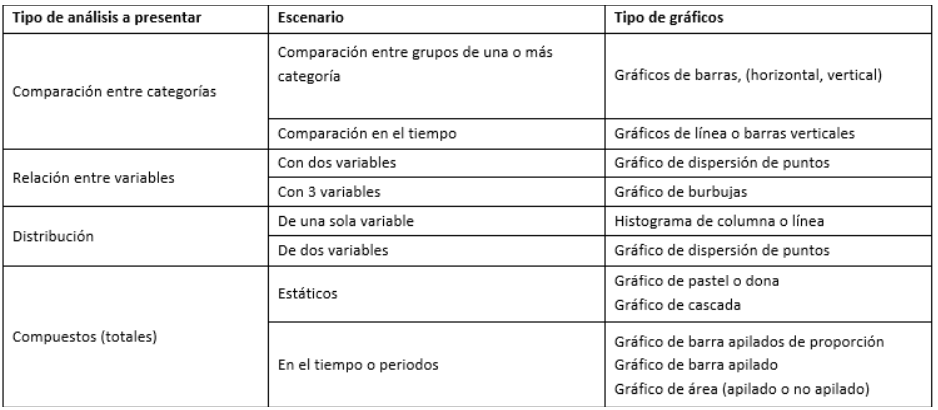
\includegraphics[keepaspectratio]{imagenes/07tablagrafp.png}}

}

\caption{Tipos de gráficos a ser usado en base los datos}

\end{figure}%

Veamos un ejemplo usando la tabla que hemos venido trabajando:

\begin{Shaded}
\begin{Highlighting}[]
\NormalTok{base\_arreglada }\SpecialCharTok{\%\textgreater{}\%}
  
  \FunctionTok{mutate}\NormalTok{(}\AttributeTok{a\_mes\_atencion=}\FunctionTok{format}\NormalTok{(fecha\_atencion, }\StringTok{"\%Y{-}\%m"}\NormalTok{)) }\SpecialCharTok{\%\textgreater{}\%} 
 
   \FunctionTok{filter}\NormalTok{(fecha\_atencion}\SpecialCharTok{\textgreater{}=}\StringTok{"2020{-}01{-}01"}\NormalTok{, fecha\_atencion}\SpecialCharTok{\textless{}}\StringTok{"2022{-}01{-}01"}\NormalTok{) }\SpecialCharTok{\%\textgreater{}\%} 
  
  \FunctionTok{tabyl}\NormalTok{(a\_mes\_atencion, condicion) }\SpecialCharTok{\%\textgreater{}\%} 
  
  \FunctionTok{adorn\_totals}\NormalTok{(}\StringTok{"col"}\NormalTok{) }\SpecialCharTok{\%\textgreater{}\%}
\FunctionTok{ggplot}\NormalTok{(}\FunctionTok{aes}\NormalTok{(}\AttributeTok{x=}\NormalTok{a\_mes\_atencion, }\AttributeTok{y=}\NormalTok{Total))}\SpecialCharTok{+} \CommentTok{\#Espacificamos lo que vamos a graficar}
  \FunctionTok{geom\_col}\NormalTok{() }\CommentTok{\#Agregamos una capa de columnas}
\end{Highlighting}
\end{Shaded}

\pandocbounded{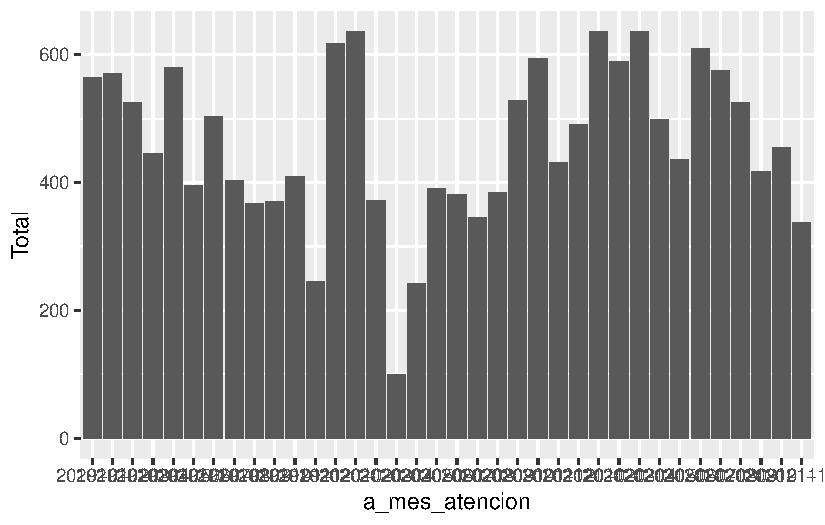
\includegraphics[keepaspectratio]{06-analisisresultados_files/figure-pdf/27-1.pdf}}

¡Tenemos nuestro primer gráfico!, pero como puedes ver, puede ser
mejorado con el fin de ser presentado en un reporte.

Lo primero que vemos que está alterado es el \textbf{eje x}, o el año y
la fecha de la notificación. Una forma de corregir esto es rotando a 45
grados el texto. A tomar en cuenta, cuando transformamos datos, usamos
el operador pipe \textbf{(\%\textgreater\%)}, en ggplot, el equivalente
es el signo de suma (\textbf{+}).

\begin{Shaded}
\begin{Highlighting}[]
\NormalTok{base\_arreglada }\SpecialCharTok{\%\textgreater{}\%}
  
  \FunctionTok{mutate}\NormalTok{(}\AttributeTok{a\_mes\_atencion=}\FunctionTok{format}\NormalTok{(fecha\_atencion, }\StringTok{"\%Y{-}\%m"}\NormalTok{)) }\SpecialCharTok{\%\textgreater{}\%} 
 
   \FunctionTok{filter}\NormalTok{(fecha\_atencion}\SpecialCharTok{\textgreater{}=}\StringTok{"2020{-}01{-}01"}\NormalTok{, fecha\_atencion}\SpecialCharTok{\textless{}}\StringTok{"2022{-}01{-}01"}\NormalTok{) }\SpecialCharTok{\%\textgreater{}\%} 
  
  \FunctionTok{tabyl}\NormalTok{(a\_mes\_atencion, condicion) }\SpecialCharTok{\%\textgreater{}\%} 
  
  \FunctionTok{adorn\_totals}\NormalTok{(}\StringTok{"col"}\NormalTok{) }\SpecialCharTok{\%\textgreater{}\%}
\FunctionTok{ggplot}\NormalTok{(}\FunctionTok{aes}\NormalTok{(}\AttributeTok{x=}\NormalTok{a\_mes\_atencion, }\AttributeTok{y=}\NormalTok{Total))}\SpecialCharTok{+} \CommentTok{\#Espacificamos lo que vamos a graficar}
  \FunctionTok{geom\_col}\NormalTok{(}\AttributeTok{color=}\StringTok{"black"}\NormalTok{, }\AttributeTok{fill=}\StringTok{"white"}\NormalTok{)}\SpecialCharTok{+} \CommentTok{\#Agregamos una capa de columnas y cambiamos el color del borde y del llenado}
  \FunctionTok{theme}\NormalTok{(}\AttributeTok{axis.text.x =} \FunctionTok{element\_text}\NormalTok{(}\AttributeTok{angle=}\DecValTok{45}\NormalTok{, }\AttributeTok{hjust=}\DecValTok{1}\NormalTok{),}
        \AttributeTok{panel.background =} \FunctionTok{element\_rect}\NormalTok{(}\AttributeTok{fill=}\StringTok{"white"}\NormalTok{)) }\CommentTok{\#en esta sección cambiamos parametros de cada elemento del gráfico, color, tamaño, etc. de elementos generales, Solo estamos modificando el texto del eje x y el color de fondo del panel.}
\end{Highlighting}
\end{Shaded}

\pandocbounded{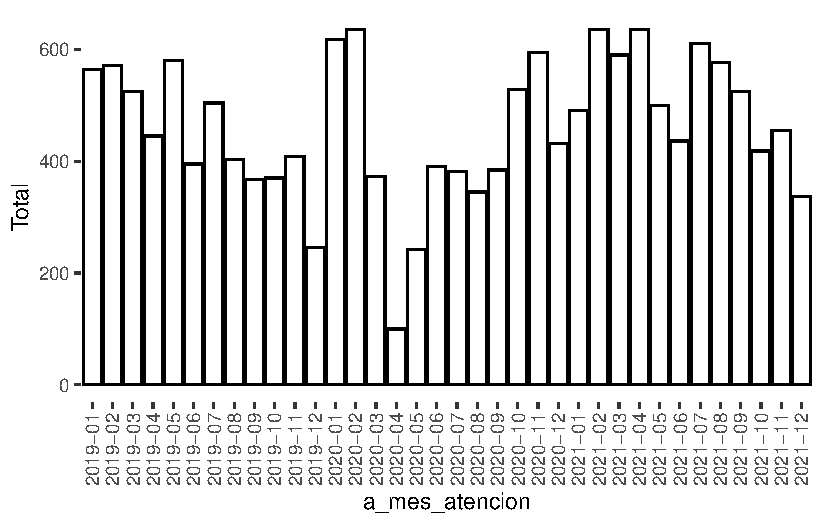
\includegraphics[keepaspectratio]{06-analisisresultados_files/figure-pdf/28-1.pdf}}

Hemos cambiado varios elementos como el color de las barras, la
presentación del texto del eje x y el color de fondo del panel. Ahora
vamos a agregar los títulos, como el título del gráfico y los de los
ejes. Para esto insertamos el comando de \textbf{labs()} que significa
labels o etiquetas.

\begin{Shaded}
\begin{Highlighting}[]
\NormalTok{base\_arreglada }\SpecialCharTok{\%\textgreater{}\%}
  
  \FunctionTok{mutate}\NormalTok{(}\AttributeTok{a\_mes\_atencion=}\FunctionTok{format}\NormalTok{(fecha\_atencion, }\StringTok{"\%Y{-}\%m"}\NormalTok{)) }\SpecialCharTok{\%\textgreater{}\%} 
 
   \FunctionTok{filter}\NormalTok{(fecha\_atencion}\SpecialCharTok{\textgreater{}=}\StringTok{"2020{-}01{-}01"}\NormalTok{, fecha\_atencion}\SpecialCharTok{\textless{}}\StringTok{"2022{-}01{-}01"}\NormalTok{) }\SpecialCharTok{\%\textgreater{}\%} 
  
  \FunctionTok{tabyl}\NormalTok{(a\_mes\_atencion, condicion) }\SpecialCharTok{\%\textgreater{}\%} 
  
  \FunctionTok{adorn\_totals}\NormalTok{(}\StringTok{"col"}\NormalTok{) }\SpecialCharTok{\%\textgreater{}\%}
\FunctionTok{ggplot}\NormalTok{(}\FunctionTok{aes}\NormalTok{(}\AttributeTok{x=}\NormalTok{a\_mes\_atencion, }\AttributeTok{y=}\NormalTok{Total))}\SpecialCharTok{+} \CommentTok{\#Espacificamos lo que vamos a graficar}
  \FunctionTok{geom\_col}\NormalTok{(}\AttributeTok{color=}\StringTok{"grey75"}\NormalTok{, }\AttributeTok{fill=}\StringTok{"white"}\NormalTok{)}\SpecialCharTok{+} \CommentTok{\#Agregamos una capa de columnas y cambiamos el color del borde y del llenado}
  \FunctionTok{labs}\NormalTok{(}\AttributeTok{title=}\StringTok{"Distribución de casos de VIH notificados"}\NormalTok{,}
       \AttributeTok{subtitle =} \StringTok{"Periodo: 2020{-}2021"}\NormalTok{,}
       \AttributeTok{x=}\StringTok{"Año y mes de diagnostico"}\NormalTok{,}
       \AttributeTok{y=}\StringTok{"Casos notificados"}\NormalTok{)}\SpecialCharTok{+}\CommentTok{\#Aquí especificamos el título, subtitulo y nombres de los ejes.}
  \FunctionTok{theme}\NormalTok{(}\AttributeTok{axis.text.x =} \FunctionTok{element\_text}\NormalTok{(}\AttributeTok{angle=}\DecValTok{45}\NormalTok{, }\AttributeTok{hjust=}\DecValTok{1}\NormalTok{),}
        \AttributeTok{panel.background =} \FunctionTok{element\_rect}\NormalTok{(}\AttributeTok{fill=}\StringTok{"white"}\NormalTok{)) }\CommentTok{\#en esta sección cambiamos parametros de cada elemento del gráfico, color, tamaño, etc. de elementos generales, Solo estamos modificando el texto del eje x y el color de fondo del panel.}
\end{Highlighting}
\end{Shaded}

\pandocbounded{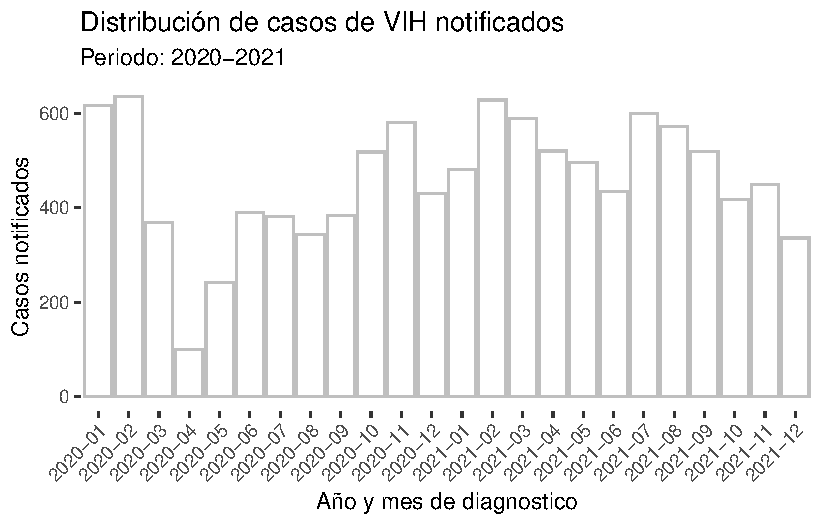
\includegraphics[keepaspectratio]{06-analisisresultados_files/figure-pdf/29-1.pdf}}

Si comparas el primer gráfico con este se nota mucho la diferencia,
(aunque todavía le falta mucho, este se puede presentar). Este seria
nuestro histograma, de hecho, hay un \textbf{geom\_} específico para los
histogramas, pero como mencioné anteriormente, para el paquete de ggplot
hay mucha documentación que básicamente se requiere un entrenamiento
aparte. Fijandote en los códigos de ejemplos y también buscando ejemplos
en la red, (ejemplo: ``como hacer un gráfico de línea con ggplot) vas a
ir aprendiendo de forma rutinaria el uso de ggplot.

También a considerar, a diferencias de las tablas, los gráficos podemos
directamente (en caso de necesitar) ya sea al clipboard o guardarlos
como imagen desde el menú de ``plots'' en el panel de archivos,
gráficos, paquetes, ayuda y visor. Para esto podemos hacer clic donde
dice ``Export'' en el menú y seleccionar ya sea guardar como imagen,
como pdf o al clipboard para pegarlo en un documento de Word o Excel o
una presentación. Si quieres cambiar el tamaño puede primero usar el
zoom o la lupa y aquí manualmente cambiar el tamaño del gráfico y hacer
un clic derecho y seleccionar guardar como (igual que desde una página
web).

\begin{figure}[H]

{\centering \pandocbounded{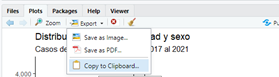
\includegraphics[keepaspectratio]{imagenes/07saveimg.png}}

}

\caption{Para exportar los gráficos de forma manual con Rstudio}

\end{figure}%

\section{Análisis de lugar}\label{anuxe1lisis-de-lugar}

Ya tenemos una tabla y un gráfico sencillo para describir el
comportamiento de los casos notificados del evento y una salida para
hacer un resumen descriptivo de los casos a través del tiempo.

Ahora vamos a ver como ha sido la distribución por zona geográfica, en
este caso las provincias de residencia de los casos. Para explorar,
vamos a construir una tabla que nos será más sencilla y tambien para
mostrar otra forma de como hacer tablas con detalles y listas para
presentar usando el paquete \textbf{gtsummary}.

Esta tabla tendrá como columnas de la provincia de residencia y otra con
el total de casos por provincia. Podemos tomar el código que usamos para
el análisis de tiempo pero con alguna variación, veamos:

\begin{Shaded}
\begin{Highlighting}[]
\NormalTok{tabla\_03 }\OtherTok{\textless{}{-}}\NormalTok{ base\_arreglada }\SpecialCharTok{\%\textgreater{}\%}
  
  \FunctionTok{mutate}\NormalTok{(}\AttributeTok{a\_mes\_atencion=}\FunctionTok{format}\NormalTok{(fecha\_atencion, }\StringTok{"\%Y{-}\%m"}\NormalTok{)) }\SpecialCharTok{\%\textgreater{}\%} 
 
   \FunctionTok{filter}\NormalTok{(fecha\_atencion}\SpecialCharTok{\textgreater{}=}\StringTok{"2020{-}01{-}01"}\NormalTok{, fecha\_atencion}\SpecialCharTok{\textless{}}\StringTok{"2022{-}01{-}01"}\NormalTok{) }\SpecialCharTok{\%\textgreater{}\%} 
  
  \FunctionTok{select}\NormalTok{(region,prov\_recla, condicion) }\SpecialCharTok{\%\textgreater{}\%} \CommentTok{\#solo seleccionamos las variables que vamos a presentar en la tabla}
  
  \FunctionTok{tbl\_summary}\NormalTok{(}\AttributeTok{by=}\NormalTok{condicion, }\AttributeTok{sort =} \FunctionTok{all\_categorical}\NormalTok{() }\SpecialCharTok{\textasciitilde{}} \StringTok{"frequency"}\NormalTok{) }\SpecialCharTok{\%\textgreater{}\%} \CommentTok{\#este es la función más básica de gtsummary (tbl\_summary), los parametros que usamos fue separar la columna condicion en sus categorias y ordenamos según la frecuencia de casos usando el parametro sort.}
  
  \FunctionTok{add\_overall}\NormalTok{() }\CommentTok{\#con esta funcion de gtsummary agregamos una columna de total}

\NormalTok{tabla\_03}
\end{Highlighting}
\end{Shaded}

\begin{table}
\fontsize{12.0pt}{14.4pt}\selectfont
\begin{tabular*}{\linewidth}{@{\extracolsep{\fill}}lccc}
\toprule
\textbf{Characteristic} & \textbf{Overall}  N = 11,030\textsuperscript{\textit{1}} & \textbf{Muerto}  N = 67\textsuperscript{\textit{1}} & \textbf{Vivo}  N = 10,963\textsuperscript{\textit{1}} \\ 
\midrule\addlinespace[2.5pt]
region &  &  &  \\ 
    O & 4,903 (44\%) & 16 (24\%) & 4,887 (45\%) \\ 
    II & 2,175 (20\%) & 39 (58\%) & 2,136 (19\%) \\ 
    V & 1,508 (14\%) & 3 (4.5\%) & 1,505 (14\%) \\ 
    III & 852 (7.7\%) & 2 (3.0\%) & 850 (7.8\%) \\ 
    I & 575 (5.2\%) & 2 (3.0\%) & 573 (5.2\%) \\ 
    VIII & 390 (3.5\%) & 2 (3.0\%) & 388 (3.5\%) \\ 
    VII & 305 (2.8\%) & 1 (1.5\%) & 304 (2.8\%) \\ 
    IV & 271 (2.5\%) & 1 (1.5\%) & 270 (2.5\%) \\ 
    VI & 51 (0.5\%) & 1 (1.5\%) & 50 (0.5\%) \\ 
prov\_recla &  &  &  \\ 
    provincias del sur & 4,563 (41\%) & 39 (58\%) & 4,524 (41\%) \\ 
    provincias centrales & 2,637 (24\%) & 6 (9.0\%) & 2,631 (24\%) \\ 
    provincia capital & 1,501 (14\%) & 10 (15\%) & 1,491 (14\%) \\ 
    provincias del norte & 1,020 (9.2\%) & 3 (4.5\%) & 1,017 (9.3\%) \\ 
    povincias occidentales & 696 (6.3\%) & 3 (4.5\%) & 693 (6.3\%) \\ 
    provincias orientales & 595 (5.4\%) & 5 (7.5\%) & 590 (5.4\%) \\ 
    resto de provincias & 18 (0.2\%) & 1 (1.5\%) & 17 (0.2\%) \\ 
\bottomrule
\end{tabular*}
\begin{minipage}{\linewidth}
\textsuperscript{\textit{1}}n (\%)\\
\end{minipage}
\end{table}

Como puedes ver en la tabla anterior, el 23\% de los casos son de la
provincia Santo Domingo, durante los 3 años que estamos describiendo.

Para tener una tabla más acabada, como por ejemplo cambiar el idioma de
los títulos a español, así como agregar una nota de pie y el título
vamos añadiendo estas funciones del paquete de \textbf{gtsummary}.

\begin{Shaded}
\begin{Highlighting}[]
 \FunctionTok{theme\_gtsummary\_language}\NormalTok{(}\AttributeTok{language =} \StringTok{"es"}\NormalTok{, }\AttributeTok{decimal.mark =} \StringTok{"."}\NormalTok{) }\CommentTok{\#esta funcion global es para decirle al paquete gtsummary que idioma usar para las tablas}
\end{Highlighting}
\end{Shaded}

\begin{verbatim}
Setting theme "language: es"
\end{verbatim}

\begin{Shaded}
\begin{Highlighting}[]
\NormalTok{tabla\_03 }\OtherTok{\textless{}{-}}\NormalTok{ base\_arreglada }\SpecialCharTok{\%\textgreater{}\%}
  
  \FunctionTok{mutate}\NormalTok{(}\AttributeTok{a\_mes\_atencion=}\FunctionTok{format}\NormalTok{(fecha\_atencion, }\StringTok{"\%Y{-}\%m"}\NormalTok{)) }\SpecialCharTok{\%\textgreater{}\%} 
 
  \FunctionTok{filter}\NormalTok{(fecha\_atencion}\SpecialCharTok{\textgreater{}=}\StringTok{"2020{-}01{-}01"}\NormalTok{, fecha\_atencion}\SpecialCharTok{\textless{}}\StringTok{"2022{-}01{-}01"}\NormalTok{) }\SpecialCharTok{\%\textgreater{}\%} 
  
  \FunctionTok{select}\NormalTok{(prov\_recla, condicion) }\SpecialCharTok{\%\textgreater{}\%} 
  
  \FunctionTok{tbl\_summary}\NormalTok{(}\AttributeTok{by=}\NormalTok{condicion, }\AttributeTok{sort =} \FunctionTok{all\_categorical}\NormalTok{() }\SpecialCharTok{\textasciitilde{}} \StringTok{"frequency"}\NormalTok{,}
              
\NormalTok{              prov\_recla}\SpecialCharTok{\textasciitilde{}}\StringTok{"Provincias de residencia de los casos"}\NormalTok{) }\SpecialCharTok{\%\textgreater{}\%}  \CommentTok{\#En la segunda linea, le cambiamos el nombre a la variable por otro nombre usando \textasciitilde{}}
  
  \FunctionTok{add\_overall}\NormalTok{() }\SpecialCharTok{\%\textgreater{}\%} 
  
  \FunctionTok{modify\_caption}\NormalTok{(}\StringTok{"**Tabla 2. Distribución de casos por provincia de residencia**"}\NormalTok{) }\SpecialCharTok{\%\textgreater{}\%} \CommentTok{\#con este comando agregamos el título a la tabla}
  
  \FunctionTok{bold\_labels}\NormalTok{() }\CommentTok{\# Con este ponemos en negritas los títulos de las categorías}




\NormalTok{tabla\_03}
\end{Highlighting}
\end{Shaded}

\begin{table}
\fontsize{12.0pt}{14.4pt}\selectfont
\begin{tabular*}{\linewidth}{@{\extracolsep{\fill}}lccc}
\toprule
\textbf{Característica} & \textbf{Global}  N = 11,030\textsuperscript{\textit{1}} & \textbf{Muerto}  N = 67\textsuperscript{\textit{1}} & \textbf{Vivo}  N = 10,963\textsuperscript{\textit{1}} \\ 
\midrule\addlinespace[2.5pt]
{\bfseries Provincias de residencia de los casos} &  &  &  \\ 
    provincias del sur & 4,563 (41\%) & 39 (58\%) & 4,524 (41\%) \\ 
    provincias centrales & 2,637 (24\%) & 6 (9.0\%) & 2,631 (24\%) \\ 
    provincia capital & 1,501 (14\%) & 10 (15\%) & 1,491 (14\%) \\ 
    provincias del norte & 1,020 (9.2\%) & 3 (4.5\%) & 1,017 (9.3\%) \\ 
    povincias occidentales & 696 (6.3\%) & 3 (4.5\%) & 693 (6.3\%) \\ 
    provincias orientales & 595 (5.4\%) & 5 (7.5\%) & 590 (5.4\%) \\ 
    resto de provincias & 18 (0.2\%) & 1 (1.5\%) & 17 (0.2\%) \\ 
\bottomrule
\end{tabular*}
\begin{minipage}{\linewidth}
\textsuperscript{\textit{1}}n (\%)\\
\end{minipage}
\end{table}

Las variables o columnas que especificamos en la función
\textbf{select()} son las que vemos en la tabla de salida. El paquete
\textbf{gtsummary} tiene muchos parámetros que nos facilita tanto para
hacer el resumen como para presentar los datos.

En el siguiente
\href{https://www.danieldsjoberg.com/gtsummary/articles/tbl_summary.html}{Tutorial}
puedes ver en más detalles todos las opciones para generar una tabla
usando \textbf{gtsummary.} Si usas Chrome o Edge, puedes traducir sin
problemas al español dado que está solo en inglés.

\section{Análisis de persona}\label{anuxe1lisis-de-persona}

En esta sección vamos a usar de nuevo la función \textbf{tbl\_summary}
del paquete \textbf{gtsummary} para hacer el resumen de persona, en este
paso toma en cuenta que desde que creamos el dataframe
\emph{base\_arreglada} tomamos las variables que vamos a usar, si nos
hacen falta, solo tenemos que actualizar este objeto. Las variables a
usar serian el \emph{sexo}, la \emph{edad}, el \emph{país de
procedencia}, el \emph{grupo de edad} y la \emph{condición de egreso},
que para los pasos anteriores la hemos usado con la finalidad de ver el
comportamiento de la letalidad.

Algo que es importante recalcar, que vaya usando como buena práctica, ve
nombrando los objetos de forma que sea fácil para identificar e integrar
en tu informe luego, por ejemplo para las tablas he usado la
nomenclatura ``tabla\_'' así será más fácil asociar el orden como
quisiera ir presentando en el informe.

\begin{Shaded}
\begin{Highlighting}[]
\NormalTok{tabla\_04 }\OtherTok{\textless{}{-}}\NormalTok{ base\_arreglada }\SpecialCharTok{\%\textgreater{}\%} 
  
\FunctionTok{mutate}\NormalTok{(}\AttributeTok{a\_mes\_atencion=}\FunctionTok{format}\NormalTok{(fecha\_atencion, }\StringTok{"\%Y{-}\%m"}\NormalTok{)) }\SpecialCharTok{\%\textgreater{}\%} 
 
   \FunctionTok{filter}\NormalTok{(fecha\_atencion}\SpecialCharTok{\textgreater{}=}\StringTok{"2020{-}01{-}01"}\NormalTok{, fecha\_atencion}\SpecialCharTok{\textless{}}\StringTok{"2022{-}01{-}01"}\NormalTok{) }\SpecialCharTok{\%\textgreater{}\%} 
  
  \FunctionTok{select}\NormalTok{(sexo, grupo\_edad,edad1, pais\_procedencia, condicion) }\SpecialCharTok{\%\textgreater{}\%}  \CommentTok{\# las variables para describir la poblacion}

  \FunctionTok{tbl\_summary}\NormalTok{(}\AttributeTok{by=}\NormalTok{sexo,}
             \AttributeTok{label =} \FunctionTok{list}\NormalTok{(grupo\_edad}\SpecialCharTok{\textasciitilde{}}\StringTok{"Grupo de edad"}\NormalTok{, }\CommentTok{\#Cuando tenemos dos o más variables que renombrar, debemos poner estas dentro de una lista}
\NormalTok{              edad1}\SpecialCharTok{\textasciitilde{}}\StringTok{"Edad en años"}\NormalTok{,}
\NormalTok{              grupo\_edad}\SpecialCharTok{\textasciitilde{}}\StringTok{"Grupo de edad en años"}\NormalTok{,}
\NormalTok{              pais\_procedencia}\SpecialCharTok{\textasciitilde{}}\StringTok{"Nacionalidad"}\NormalTok{,}
\NormalTok{              condicion}\SpecialCharTok{\textasciitilde{}}\StringTok{"Condición de Egreso"}\NormalTok{)) }\SpecialCharTok{\%\textgreater{}\%} 
  \FunctionTok{add\_overall}\NormalTok{() }\SpecialCharTok{\%\textgreater{}\%} 
  \FunctionTok{modify\_caption}\NormalTok{(}\StringTok{"**Tabla 3. Distribución de casos según características**"}\NormalTok{) }\SpecialCharTok{\%\textgreater{}\%} 
  \FunctionTok{bold\_labels}\NormalTok{()}

\NormalTok{tabla\_04}
\end{Highlighting}
\end{Shaded}

\begin{table}
\fontsize{12.0pt}{14.4pt}\selectfont
\begin{tabular*}{\linewidth}{@{\extracolsep{\fill}}lccc}
\toprule
\textbf{Característica} & \textbf{Global}  N = 11,030\textsuperscript{\textit{1}} & \textbf{Femenino}  N = 5,577\textsuperscript{\textit{1}} & \textbf{Masculino}  N = 5,453\textsuperscript{\textit{1}} \\ 
\midrule\addlinespace[2.5pt]
{\bfseries Grupo de edad en años} &  &  &  \\ 
    <1 & 2 (<0.1\%) & 2 (<0.1\%) & 0 (0\%) \\ 
    1\_4 & 72 (0.7\%) & 28 (0.5\%) & 44 (0.8\%) \\ 
    10\_19 & 464 (4.2\%) & 310 (5.6\%) & 154 (2.8\%) \\ 
    20\_29 & 2,931 (27\%) & 1,673 (30\%) & 1,258 (23\%) \\ 
    30\_39 & 3,006 (27\%) & 1,514 (27\%) & 1,492 (27\%) \\ 
    40\_49 & 2,302 (21\%) & 1,080 (19\%) & 1,222 (22\%) \\ 
    5\_9 & 36 (0.3\%) & 17 (0.3\%) & 19 (0.3\%) \\ 
    50\_59 & 1,347 (12\%) & 589 (11\%) & 758 (14\%) \\ 
    60 o más & 870 (7.9\%) & 364 (6.5\%) & 506 (9.3\%) \\ 
{\bfseries Edad en años} & 36 (27, 47) & 34 (26, 45) & 38 (29, 48) \\ 
{\bfseries Nacionalidad} &  &  &  \\ 
    1 & 9,070 (82\%) & 4,464 (80\%) & 4,606 (84\%) \\ 
    2 & 1,910 (17\%) & 1,100 (20\%) & 810 (15\%) \\ 
    3 & 50 (0.5\%) & 13 (0.2\%) & 37 (0.7\%) \\ 
{\bfseries Condición de Egreso} &  &  &  \\ 
    Muerto & 67 (0.6\%) & 20 (0.4\%) & 47 (0.9\%) \\ 
    Vivo & 10,963 (99\%) & 5,557 (100\%) & 5,406 (99\%) \\ 
\bottomrule
\end{tabular*}
\begin{minipage}{\linewidth}
\textsuperscript{\textit{1}}n (\%); Mediana (Q1, Q3)\\
\end{minipage}
\end{table}

Algo a notar cuando generamos la tabla es que el grupo de edad no esta
ordenado y también se puede mejorar su presentación, para corregir vamos
a volver al proceso de ``limpieza'' y usamos de nuevo la función
\textbf{case\_when().} Podemos ver que hay una categoría que no sale en
orden (5\_9a) para corregir esto como funciona case\_when es valor
actual (grupo\_edad==``5\_9'') seguido de una virgulilla
(\textasciitilde) y el nuevo valor (sugerencia: ``05-09'') y para el
último valor ya sea mantener el resto de los valores se usa TRUE
\textasciitilde{} nombre de la variable, también las categoría de esta
variable tienen como separador de los rangos de edades ``\_'' y queremos
poner ``-'', para esto usamos la función \textbf{str\_replace()} de
tidyverse donde especificamos la variable, luego el termino a ser
buscado y luego el termino de reemplazo.

\begin{Shaded}
\begin{Highlighting}[]
\NormalTok{tabla\_04 }\OtherTok{\textless{}{-}}\NormalTok{ base\_arreglada }\SpecialCharTok{\%\textgreater{}\%} 
  
\FunctionTok{mutate}\NormalTok{(}\AttributeTok{a\_mes\_atencion=}\FunctionTok{format}\NormalTok{(fecha\_atencion, }\StringTok{"\%Y{-}\%m"}\NormalTok{),}
       
       \AttributeTok{grupo\_edad=}\FunctionTok{case\_when}\NormalTok{(grupo\_edad}\SpecialCharTok{==}\StringTok{"\textless{}1"}\SpecialCharTok{\textasciitilde{}}\StringTok{"00{-}01"}\NormalTok{,}
\NormalTok{                            grupo\_edad}\SpecialCharTok{==}\StringTok{"1\_4"}\SpecialCharTok{\textasciitilde{}}\StringTok{"01{-}04"}\NormalTok{,}
\NormalTok{                            grupo\_edad}\SpecialCharTok{==}\StringTok{"5\_9"}\SpecialCharTok{\textasciitilde{}}\StringTok{"05{-}09"}\NormalTok{,}
                            \ConstantTok{TRUE}\SpecialCharTok{\textasciitilde{}}\NormalTok{grupo\_edad),}
       
       \AttributeTok{grupo\_edad=}\FunctionTok{str\_replace}\NormalTok{(grupo\_edad,}\StringTok{"\_"}\NormalTok{,}\StringTok{" {-} "}\NormalTok{)}
       
\NormalTok{       ) }\SpecialCharTok{\%\textgreater{}\%} \CommentTok{\#aqui cambiamos el underscore por el dash con la funcion str\_replace}
 
   \FunctionTok{filter}\NormalTok{(fecha\_atencion}\SpecialCharTok{\textgreater{}=}\StringTok{"2019{-}01{-}01"}\NormalTok{, fecha\_atencion}\SpecialCharTok{\textless{}}\StringTok{"2022{-}01{-}01"}\NormalTok{) }\SpecialCharTok{\%\textgreater{}\%}
  
  
  \FunctionTok{select}\NormalTok{(sexo, grupo\_edad,edad1, pais\_procedencia, condicion) }\SpecialCharTok{\%\textgreater{}\%}  \CommentTok{\# las variables para describir la poblacion}

  \FunctionTok{tbl\_summary}\NormalTok{(}\AttributeTok{by=}\NormalTok{sexo,}
             \AttributeTok{label =} \FunctionTok{list}\NormalTok{(grupo\_edad}\SpecialCharTok{\textasciitilde{}}\StringTok{"Grupo de edad"}\NormalTok{, }\CommentTok{\#Cuando tenemos dos o más variables que renombrar, debemos poner estas dentro de una lista}
\NormalTok{              edad1}\SpecialCharTok{\textasciitilde{}}\StringTok{"Edad en años"}\NormalTok{,}
\NormalTok{              grupo\_edad}\SpecialCharTok{\textasciitilde{}}\StringTok{"Grupo de edad en años"}\NormalTok{,}
\NormalTok{              pais\_procedencia}\SpecialCharTok{\textasciitilde{}}\StringTok{"Nacionalidad"}\NormalTok{,}
\NormalTok{              condicion}\SpecialCharTok{\textasciitilde{}}\StringTok{"Condición de Egreso"}\NormalTok{)) }\SpecialCharTok{\%\textgreater{}\%} 
  \FunctionTok{add\_overall}\NormalTok{() }\SpecialCharTok{\%\textgreater{}\%} 
  \FunctionTok{modify\_caption}\NormalTok{(}\StringTok{"**Tabla 4. Distribución de casos según características**"}\NormalTok{) }\SpecialCharTok{\%\textgreater{}\%} 
  \FunctionTok{bold\_labels}\NormalTok{()}

\NormalTok{tabla\_04}
\end{Highlighting}
\end{Shaded}

\begin{table}
\fontsize{12.0pt}{14.4pt}\selectfont
\begin{tabular*}{\linewidth}{@{\extracolsep{\fill}}lccc}
\toprule
\textbf{Característica} & \textbf{Global}  N = 16,394\textsuperscript{\textit{1}} & \textbf{Femenino}  N = 8,357\textsuperscript{\textit{1}} & \textbf{Masculino}  N = 8,037\textsuperscript{\textit{1}} \\ 
\midrule\addlinespace[2.5pt]
{\bfseries Grupo de edad en años} &  &  &  \\ 
    00-01 & 2 (<0.1\%) & 2 (<0.1\%) & 0 (0\%) \\ 
    01-04 & 91 (0.6\%) & 38 (0.5\%) & 53 (0.7\%) \\ 
    05-09 & 45 (0.3\%) & 24 (0.3\%) & 21 (0.3\%) \\ 
    10 - 19 & 720 (4.4\%) & 484 (5.8\%) & 236 (2.9\%) \\ 
    20 - 29 & 4,503 (27\%) & 2,571 (31\%) & 1,932 (24\%) \\ 
    30 - 39 & 4,556 (28\%) & 2,324 (28\%) & 2,232 (28\%) \\ 
    40 - 49 & 3,375 (21\%) & 1,593 (19\%) & 1,782 (22\%) \\ 
    50 - 59 & 1,928 (12\%) & 833 (10.0\%) & 1,095 (14\%) \\ 
    60 o más & 1,174 (7.2\%) & 488 (5.8\%) & 686 (8.5\%) \\ 
{\bfseries Edad en años} & 35 (27, 46) & 34 (26, 44) & 37 (29, 48) \\ 
{\bfseries Nacionalidad} &  &  &  \\ 
    1 & 13,414 (82\%) & 6,630 (79\%) & 6,784 (84\%) \\ 
    2 & 2,899 (18\%) & 1,712 (20\%) & 1,187 (15\%) \\ 
    3 & 81 (0.5\%) & 15 (0.2\%) & 66 (0.8\%) \\ 
{\bfseries Condición de Egreso} &  &  &  \\ 
    Muerto & 76 (0.5\%) & 24 (0.3\%) & 52 (0.6\%) \\ 
    Vivo & 16,318 (100\%) & 8,333 (100\%) & 7,985 (99\%) \\ 
\bottomrule
\end{tabular*}
\begin{minipage}{\linewidth}
\textsuperscript{\textit{1}}n (\%); Mediana (Q1, Q3)\\
\end{minipage}
\end{table}

Ahora con este mismo resumen que usamos para la tabla anterior, vamos a
hacer un gráfico de grupos de edades por sexo, que usamos de forma común
para describir la población de cualquier evento. Continuando un poco con
\textbf{ggplot}

\begin{figure}[H]

{\centering \pandocbounded{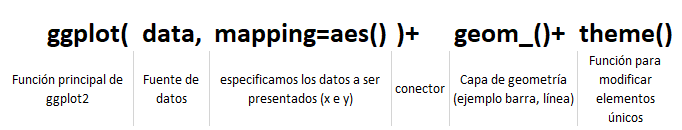
\includegraphics[keepaspectratio]{imagenes/07ggplot.png}}

}

\caption{Anatomía de la función de ggplot}

\end{figure}%

Aparte de lo presentado en la imagen anterior, existen otras funciones
complementarias como scale (\textbf{scale\_}) que ayudan al ajuste del
gráfico, pero mientras tanto, solo vamos a enfocarnos en lo básico.

En el gráfico que hicimos de tiempo solo presentamos una variable. En
este ejemplo, vamos a presentar una variable con dos o más categorías
para mostrar una funcionalidad muy importante de la función de
\textbf{ggplot}.

\begin{Shaded}
\begin{Highlighting}[]
\CommentTok{\#primero hacemos una tabla resumen con solo grupo edad y sexo}
\NormalTok{grafico\_edad\_reco }\OtherTok{\textless{}{-}}\NormalTok{ base\_arreglada }\SpecialCharTok{\%\textgreater{}\%} 
  \FunctionTok{mutate}\NormalTok{(}\AttributeTok{grupo\_edad=}\FunctionTok{case\_when}\NormalTok{(grupo\_edad}\SpecialCharTok{==}\StringTok{"1\_4"}\SpecialCharTok{\textasciitilde{}}\StringTok{"01\_04"}\NormalTok{,}
\NormalTok{                              grupo\_edad}\SpecialCharTok{==}\StringTok{"5\_9"}\SpecialCharTok{\textasciitilde{}}\StringTok{"05\_09"}\NormalTok{,}
                              \ConstantTok{TRUE}\SpecialCharTok{\textasciitilde{}}\NormalTok{grupo\_edad)) }\SpecialCharTok{\%\textgreater{}\%} 
  \FunctionTok{select}\NormalTok{(grupo\_edad, sexo) }\SpecialCharTok{\%\textgreater{}\%}
  \FunctionTok{group\_by}\NormalTok{(grupo\_edad, sexo) }\SpecialCharTok{\%\textgreater{}\%}  \CommentTok{\#agrupamos por estas dos variables}
  \FunctionTok{count}\NormalTok{() }\SpecialCharTok{\%\textgreater{}\%}  \CommentTok{\#realizamos una cuenta de estas dos variables, el resultado es un dataframe con 3 variables (grupo\_edad, sexo y n o cuenta)}
  \FunctionTok{ggplot}\NormalTok{(}\FunctionTok{aes}\NormalTok{(}\AttributeTok{x=}\NormalTok{grupo\_edad, }\AttributeTok{y=}\NormalTok{n, }\AttributeTok{fill=}\NormalTok{sexo))}\SpecialCharTok{+} \CommentTok{\# como estamos conectando el resumen con la función de ggplot, no necesitamos especificar el parametro data= o fuente de datos}
\FunctionTok{geom\_col}\NormalTok{()}

\CommentTok{\#veamos el gráfico }
\NormalTok{grafico\_edad\_reco}
\end{Highlighting}
\end{Shaded}

\pandocbounded{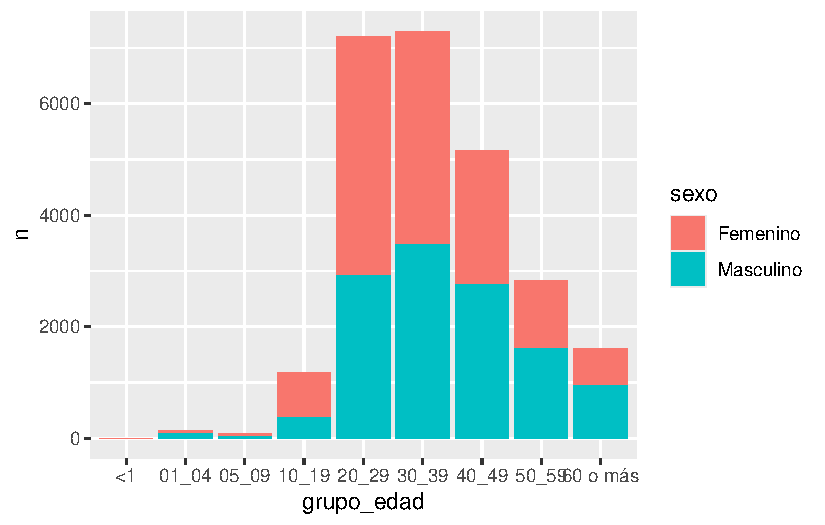
\includegraphics[keepaspectratio]{06-analisisresultados_files/figure-pdf/36-1.pdf}}

Al igual con el ejemplo anterior, antes de usar este gráfico para
presentar podemos hacer cambios, ejemplo, las barras que representa cada
sexo por separado, el color de relleno también.

\begin{Shaded}
\begin{Highlighting}[]
\NormalTok{grafico\_edad\_reco }\OtherTok{\textless{}{-}}\NormalTok{ base\_arreglada }\SpecialCharTok{\%\textgreater{}\%} 
  \FunctionTok{mutate}\NormalTok{(}\AttributeTok{grupo\_edad=}\FunctionTok{case\_when}\NormalTok{(grupo\_edad}\SpecialCharTok{==}\StringTok{"1\_4"}\SpecialCharTok{\textasciitilde{}}\StringTok{"01\_04"}\NormalTok{,}
\NormalTok{                              grupo\_edad}\SpecialCharTok{==}\StringTok{"5\_9"}\SpecialCharTok{\textasciitilde{}}\StringTok{"05\_09"}\NormalTok{,}
                              \ConstantTok{TRUE}\SpecialCharTok{\textasciitilde{}}\NormalTok{grupo\_edad)) }\SpecialCharTok{\%\textgreater{}\%} 
  \FunctionTok{select}\NormalTok{(grupo\_edad, sexo) }\SpecialCharTok{\%\textgreater{}\%}
  \FunctionTok{group\_by}\NormalTok{(grupo\_edad, sexo) }\SpecialCharTok{\%\textgreater{}\%} 
  \FunctionTok{count}\NormalTok{() }\SpecialCharTok{\%\textgreater{}\%}  
  \FunctionTok{ggplot}\NormalTok{(}\FunctionTok{aes}\NormalTok{(}\AttributeTok{x=}\NormalTok{grupo\_edad, }
             \AttributeTok{y=}\NormalTok{n, }
             \AttributeTok{fill=}\NormalTok{sexo))}\SpecialCharTok{+} \CommentTok{\#fill es relleno, }
\FunctionTok{geom\_col}\NormalTok{(}\AttributeTok{color=}\StringTok{"black"}\NormalTok{,     }\CommentTok{\#agregamos color al borde}
         \AttributeTok{position =} \StringTok{"dodge"}\NormalTok{)}\SpecialCharTok{+} \CommentTok{\#especificamos que la variable sexo será en columnas separadas, no apiladas}
\FunctionTok{scale\_fill\_manual}\NormalTok{(}\AttributeTok{values=}\FunctionTok{c}\NormalTok{(}\StringTok{"Femenino"}\OtherTok{=}\StringTok{"white"}\NormalTok{,}
                           \StringTok{"Masculino"}\OtherTok{=}\StringTok{"grey"}\NormalTok{))}\SpecialCharTok{+}\CommentTok{\#con esta función de ayuda podemos manualmente cambiar los colores de relleno, con el parametro values=creamos un vector con las categorias y le asignamos un color.}
\FunctionTok{theme\_minimal}\NormalTok{() }\CommentTok{\#este es un tema (theme) que trae ggplot, hay paquetes que tienen temas mucho más acabado, }
\NormalTok{grafico\_edad\_reco}
\end{Highlighting}
\end{Shaded}

\pandocbounded{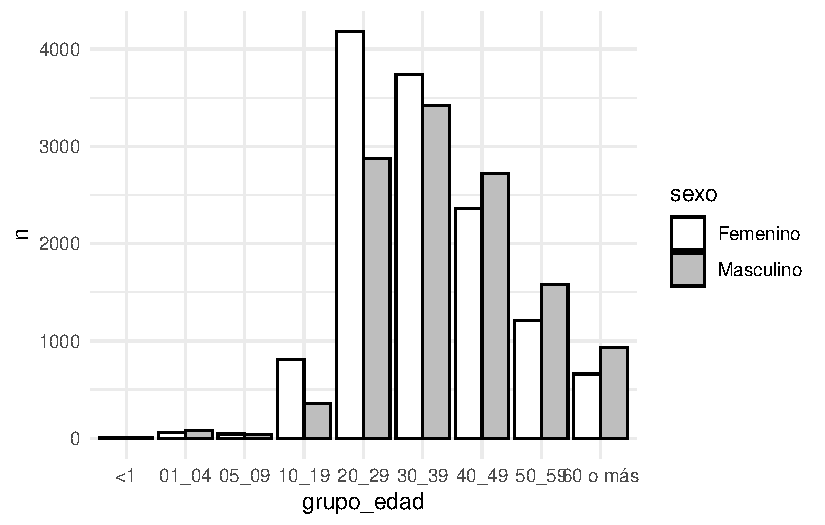
\includegraphics[keepaspectratio]{06-analisisresultados_files/figure-pdf/37-1.pdf}}

Todavía hay muchos elementos que cambiar pero te dejo de tarea que
busques lo siguiente:

\begin{itemize}
\item
  ¿Cómo agregar un separador de miles al número del eje y?
\item
  ¿Cómo cambiar los títulos de los ejes y agregar título del gráfico?.
  (ver ejemplo del análisis de tiempo)
\item
  ¿Cómo puedo cambiar los colores del relleno de las barras?. ¿Cómo
  puedo remover o agregar las líneas guía en el fondo del gráfico?
\end{itemize}

La idea es que puedas también ir desarrollando la habilidad de usar las
referencias que están disponible. Realmente no debes de aprenderte todos
los comandos y funciones, lo que debes de tomar siempre en cuenta es
definir bien \textbf{que es lo que necesitas o quieres} para luego
tratar de procesarlo, esto lo mencioné al inicio de este manual.

Ahora que tenemos algunos elementos para comenzar un análisis
descriptivo podemos comenzar a trabajar como ponerlos en un mismo
documento usando \textbf{rmarkdown}.

\section{Evaluando si existe relación entre la variable dependiente e
independiente}\label{evaluando-si-existe-relaciuxf3n-entre-la-variable-dependiente-e-independiente}

En este ejercicio en los pasos anteriores pudimos hacer un poco de
analisis exploratorio, descriptivo, ahora brevemente vamos a realizar un
análisis de estadística inferencial usando regresión lineal. Para esto
bien sabes que la regresión lineal es un método aplicable en muchas
situaciones en las que se estudia la relación entre dos o más variables
o predecir un comportamiento, y para esto vamos a usar dos variables que
sean \textbf{continuas}.

Vamos a evaluar si existe relación entre el año de ocurrencia de casos y
la cantidad de casos y tambien predecir la cantidad de casos para años
futuros, para esto tenemos que hacer una transformación de los datos.
Primero vamos a crear un nuevo dataframe o una tabla resumen a partir
del dataframe de la base arreglada:

\begin{Shaded}
\begin{Highlighting}[]
\NormalTok{casos\_por\_ann }\OtherTok{\textless{}{-}}\NormalTok{ base\_arreglada }\SpecialCharTok{\%\textgreater{}\%} \CommentTok{\#nueva tabla}
  \FunctionTok{group\_by}\NormalTok{(ano\_atencion) }\SpecialCharTok{\%\textgreater{}\%}        \CommentTok{\#agrupamos por año del caso}
  \FunctionTok{count}\NormalTok{()                           }\CommentTok{\#hacemos un conteo de casos (cada fila) por año}


\NormalTok{casos\_por\_ann}
\end{Highlighting}
\end{Shaded}

\begin{verbatim}
# A tibble: 5 x 2
# Groups:   ano_atencion [5]
  ano_atencion     n
         <dbl> <int>
1         2017  4035
2         2018  4613
3         2019  5352
4         2020  5008
5         2021  6039
\end{verbatim}

Como podemos ver tenemos una nueva tabla que tiene dos columnas, la de
los años (ano\_atencion o variable independiente) y la del total de
casos (n o variable dependiente). Ahora vamos a construir un nuevo
objeto que tendrá el resumen del análisis de la regresión lineal, para
esto vamos a usar la función \textbf{lm()} del paquete \{base\} de R.
Los argumentos para esta formula son la base de datos, la variable
independiente seguida del simbolo ``\textasciitilde{}'' o virgulilla y
luego las variables independientes, cada una separada por el simbolo
``+'' en caso de ser más de una variable independiente. Luego de crear
el objeto de regresión lineal o lm, para ver los resultados usamos la
función \textbf{summary()} para ver los resultados con más detalles del
modelo de regresión.

\begin{Shaded}
\begin{Highlighting}[]
\NormalTok{modelo\_reg\_lin }\OtherTok{\textless{}{-}} \FunctionTok{lm}\NormalTok{(}\AttributeTok{data=}\NormalTok{casos\_por\_ann, n}\SpecialCharTok{\textasciitilde{}}\NormalTok{ano\_atencion) }

\FunctionTok{summary}\NormalTok{(modelo\_reg\_lin)}
\end{Highlighting}
\end{Shaded}

\begin{verbatim}

Call:
lm(formula = n ~ ano_atencion, data = casos_por_ann)

Residuals:
     1      2      3      4      5 
 -93.8   43.9  342.6 -441.7  149.0 

Coefficients:
              Estimate Std. Error t value Pr(>|t|)  
(Intercept)  -883956.3   216639.3  -4.080   0.0266 *
ano_atencion     440.3      107.3   4.103   0.0262 *
---
Signif. codes:  0 '***' 0.001 '**' 0.01 '*' 0.05 '.' 0.1 ' ' 1

Residual standard error: 339.3 on 3 degrees of freedom
Multiple R-squared:  0.8488,    Adjusted R-squared:  0.7984 
F-statistic: 16.84 on 1 and 3 DF,  p-value: 0.02619
\end{verbatim}

Según la salida que nos muestra la consola tenemos que por cada año que
pasa, la variable dependiente (casos) aumenta en 440.3 casos y el valor
de R al cuadrado (coeficiente de correlación) es de \textbf{0.7983689}
que significa que el 77\% de la variable dependiente se puede explicar
por la variable independiente. Verifica el valor de p, este al parecer
es menor de 0.05, lo que si hubiésemos planteado una hipótesis nula (no
hay relación entre ambas variables) podemos rechazarla y quedarnos con
la hipótesis alterna (hay relación significativa entre ambas variables).

Supongamos que ahora quisiéramos saber en los años posteriores a los que
tenemos en la base resumen de los casos por año, digamos que en los
próximos 5 años, como se comportarían los casos reportados, pudiéramos
usar la función \textbf{predict()} de \{base\}. Primero vamos a crear un
nuevo dataframe con los años futuros y luego vamos a usar el modelo de
regresión lineal y le pasamos este nuevo dataframe, así:

\begin{Shaded}
\begin{Highlighting}[]
\CommentTok{\#nuevo dataframe (5 años)}

\NormalTok{ann\_futuros }\OtherTok{\textless{}{-}} \FunctionTok{data.frame}\NormalTok{(}\AttributeTok{ano\_atencion=}\FunctionTok{c}\NormalTok{(}\DecValTok{2022}\SpecialCharTok{:}\DecValTok{2026}\NormalTok{))}

\CommentTok{\# prediccion}

\NormalTok{prediccion }\OtherTok{\textless{}{-}} \FunctionTok{predict}\NormalTok{(modelo\_reg\_lin, ann\_futuros)}

\FunctionTok{names}\NormalTok{(prediccion) }\OtherTok{\textless{}{-}}\NormalTok{ ann\_futuros}\SpecialCharTok{$}\NormalTok{ano\_atencion }\CommentTok{\#para agregar el nombre o el año}

\NormalTok{prediccion}
\end{Highlighting}
\end{Shaded}

\begin{verbatim}
  2022   2023   2024   2025   2026 
6330.3 6770.6 7210.9 7651.2 8091.5 
\end{verbatim}

Si queremos agregar las predicciones al dataframe resumen de los años y
casos, debemos convertir el vector \emph{prediccion} en dataframe
(usando la función data.frame) y luego unirlo al dataframe resumen.

\begin{Shaded}
\begin{Highlighting}[]
\NormalTok{pred\_df }\OtherTok{\textless{}{-}} \FunctionTok{data.frame}\NormalTok{(prediccion) }\SpecialCharTok{\%\textgreater{}\%} 
  \FunctionTok{rownames\_to\_column}\NormalTok{() }\SpecialCharTok{\%\textgreater{}\%}  \CommentTok{\#aplicamos la función rownames\_to\_columns para agregar la columna de años}
  \FunctionTok{rename}\NormalTok{(}\AttributeTok{ano\_atencion=}\DecValTok{1}\NormalTok{, }\AttributeTok{n=}\DecValTok{2}\NormalTok{) }\SpecialCharTok{\%\textgreater{}\%}  \CommentTok{\#corregimos los nombres (importante antes de unir las tablas)}
  \FunctionTok{mutate}\NormalTok{(}\AttributeTok{ano\_atencion=}\FunctionTok{as.numeric}\NormalTok{(ano\_atencion)) }\CommentTok{\#convertimos a tipo numerico la columna de años}

\NormalTok{nuevo\_df }\OtherTok{\textless{}{-}}\NormalTok{ casos\_por\_ann }\SpecialCharTok{\%\textgreater{}\%}  \CommentTok{\#la base original}
  \FunctionTok{bind\_rows}\NormalTok{(pred\_df) }\CommentTok{\#unimos la base nueva con las predicciones}

\NormalTok{nuevo\_df}
\end{Highlighting}
\end{Shaded}

\begin{verbatim}
# A tibble: 10 x 2
# Groups:   ano_atencion [10]
   ano_atencion     n
          <dbl> <dbl>
 1         2017 4035 
 2         2018 4613 
 3         2019 5352 
 4         2020 5008 
 5         2021 6039 
 6         2022 6330.
 7         2023 6771.
 8         2024 7211.
 9         2025 7651.
10         2026 8092.
\end{verbatim}

Esta es una muestra de como podemos hacer un análisis de estadistica
inferencial. Hay muchos otros que podemos hacer, te recomiendo que
revises los temas que te interesan dominar sobre análisis estadístico y
busca como puedes llevarlos a cabo usando R, vas a encontrar una gran
cantidad de ejemplos.

Este que vimos es un solo abordaje, y dependiendo de tus objetivos puede
aplicar otros.

\bookmarksetup{startatroot}

\chapter{Preparación de reporte (integración de las salidas en un
documento)}\label{preparaciuxf3n-de-reporte-integraciuxf3n-de-las-salidas-en-un-documento}

\section{Introducción a Rmarkdown}\label{introducciuxf3n-a-rmarkdown}

En este capítulo vamos a ver como integramos los elementos de nuestro
análisis (tablas, gráficos) y la descripción así como la intepretación
de los datos. Reportar es uno de los pasos más importantes cuando
trabajamos en esta área, y contar con herramientas que nos faciliten
esta tarea nos da la gran ventaja de ahorrar tiempo. Por ejemplo poder
prepararar un manuscrito, la presentación, (hasta un poster!) en un solo
lugar es posible con R a través de RMarkdown que es una herramienta
poderosa dentro del ecosistema de RStudio (este manual fue realizado
usando RMarkdown).

Para profesionales de la salud que realizan análisis de datos, RMarkdown
ofrece una solución ideal para crear informes reproducibles, compartir
hallazgos y documentar adecuadamente los procesos analíticos.

En este capítulo, aprenderás cómo utilizar RMarkdown para crear
documentos bien acabados en diferentes formatos (docx, pdf, html) que
integren análisis estadísticos, visualizaciones y texto.

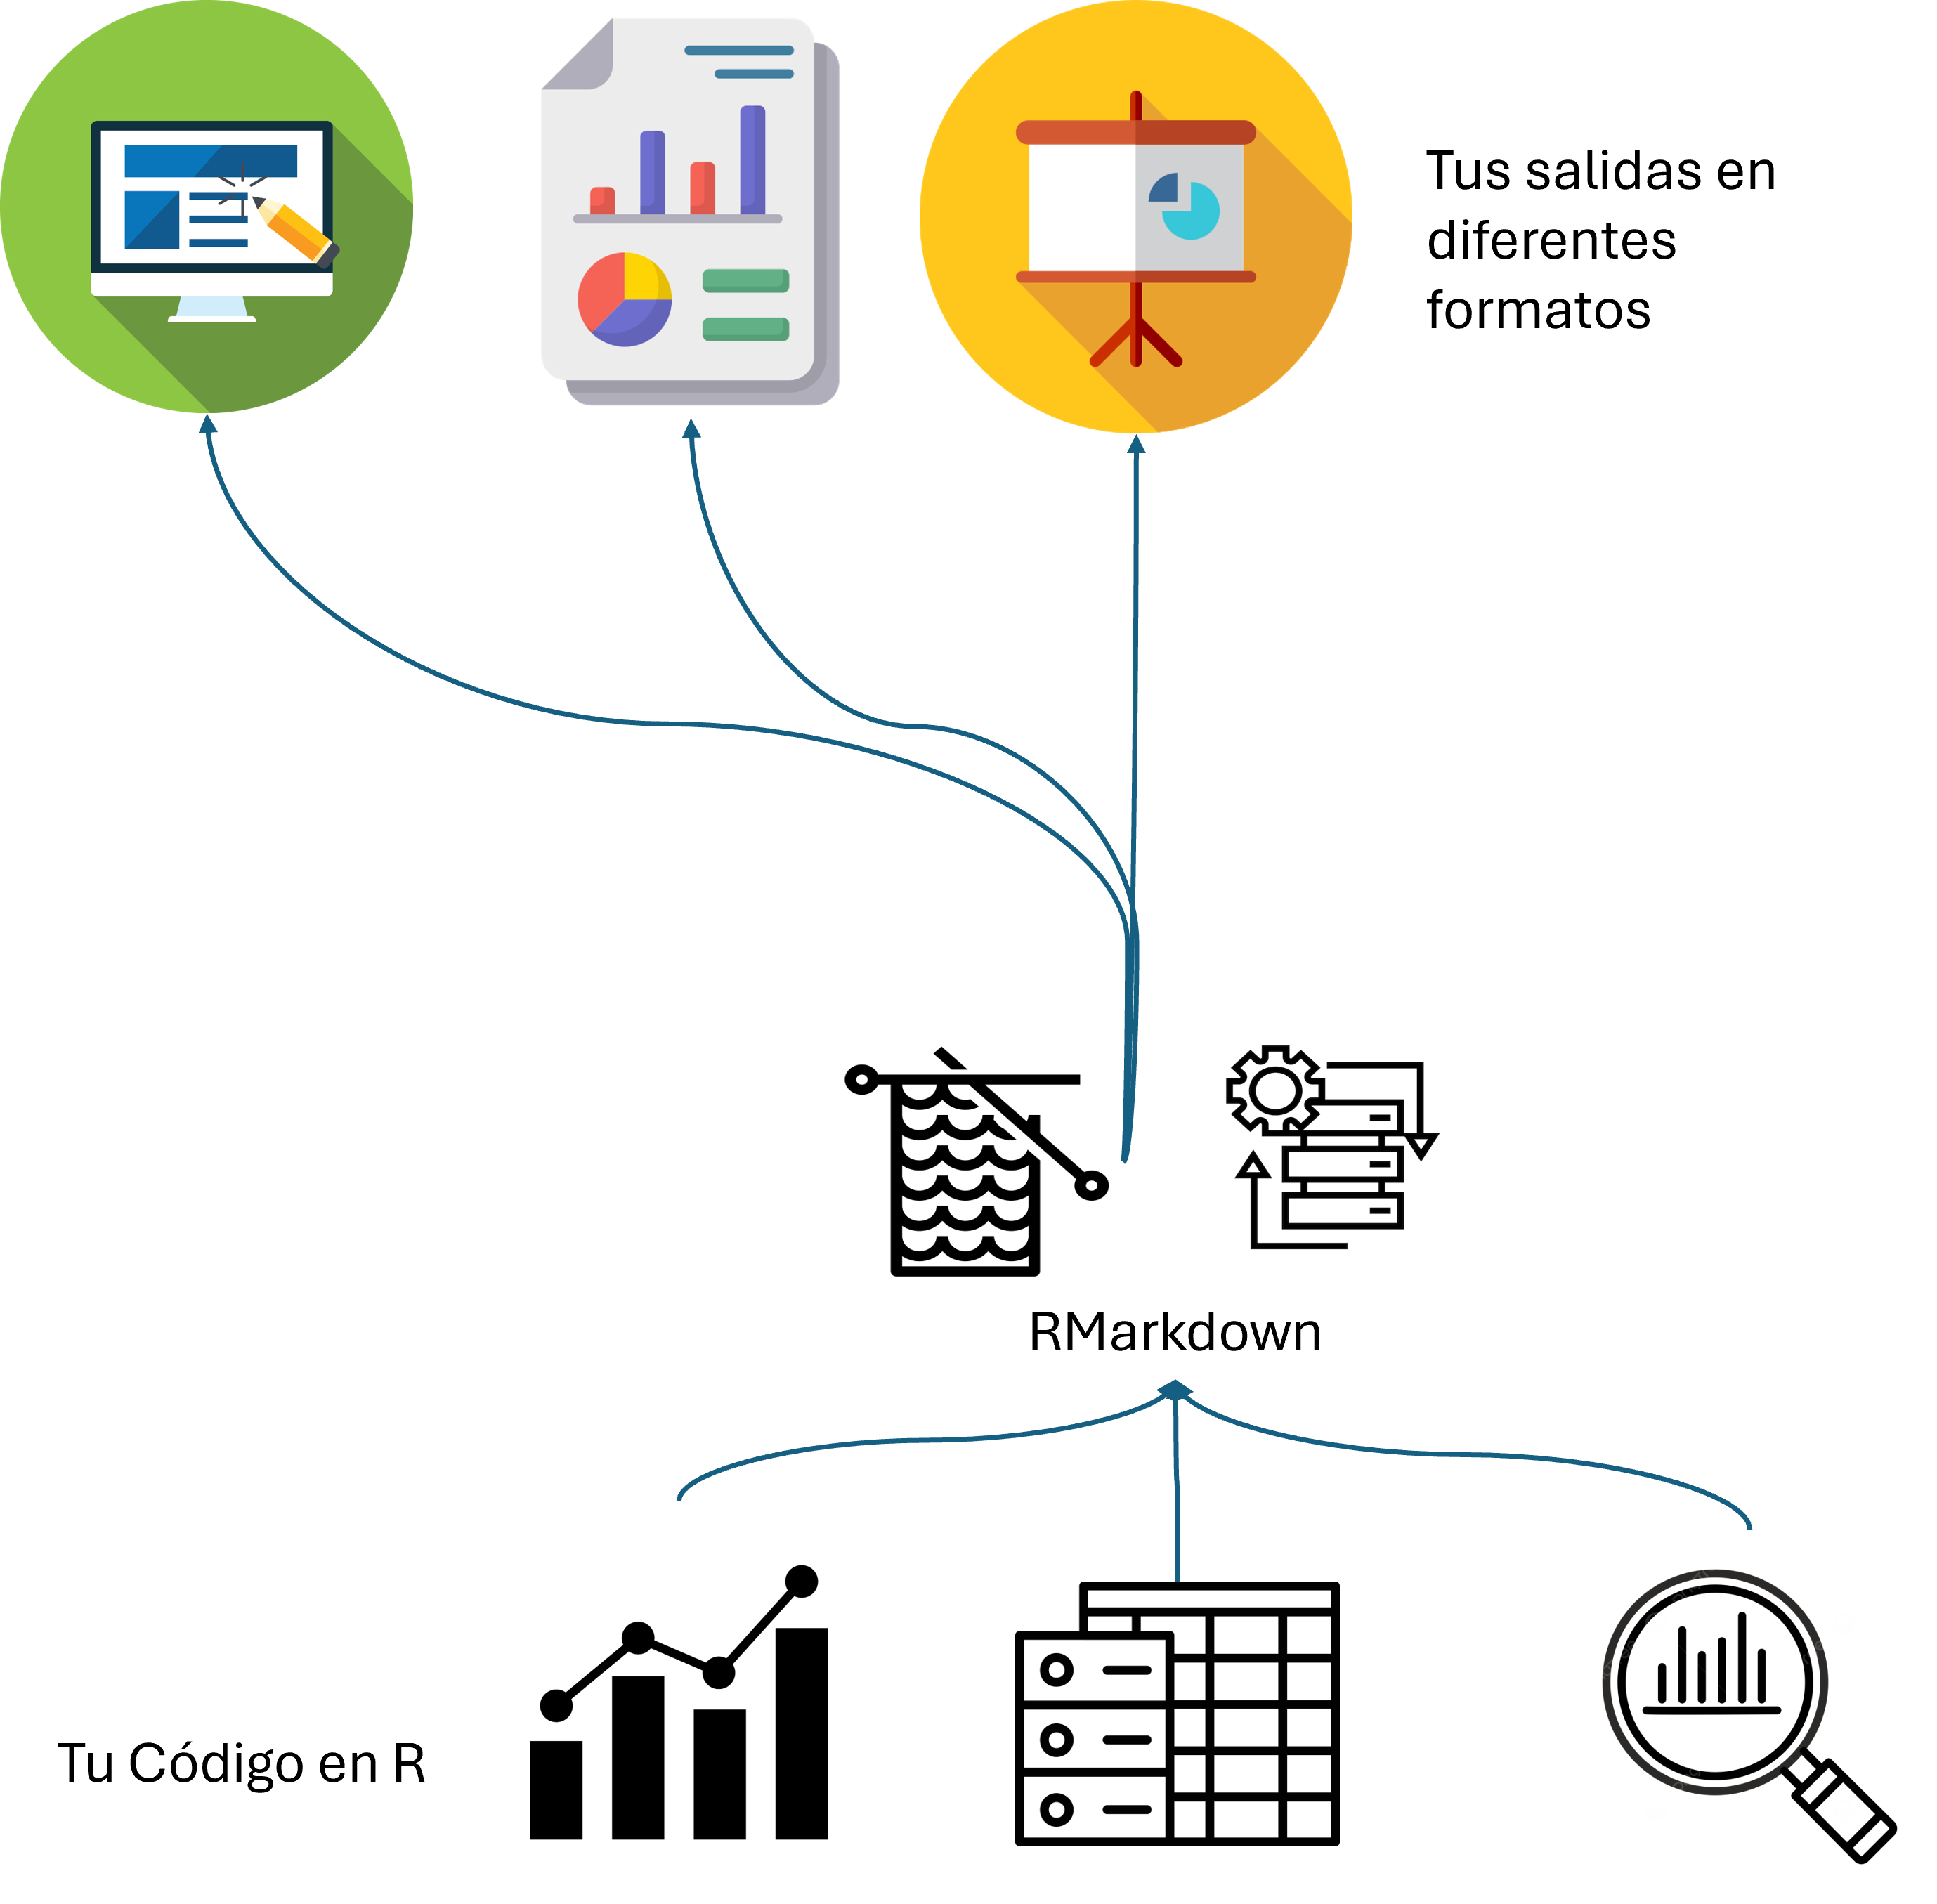
\includegraphics[width=5in,height=\textheight,keepaspectratio]{imagenes/08rmarkdown.png}

\section{¿Qué es RMarkdown y por qué
usarlo?}\label{quuxe9-es-rmarkdown-y-por-quuxe9-usarlo}

RMarkdown es un formato que combina la sintaxis de Markdown (un lenguaje
de etiqueta) con la capacidad de ejecutar código R. Sus principales
ventajas para profesionales de la salud incluyen:

\begin{enumerate}
\def\labelenumi{\arabic{enumi}.}
\tightlist
\item
  \textbf{Reproducibilidad}: Los análisis pueden ser replicados
  exactamente por otros investigadores.
\item
  \textbf{Transparencia}: Todos los pasos del análisis están
  documentados.
\item
  \textbf{Integración}: Código, resultados, visualizaciones y texto
  explicativo en un solo documento.
\item
  \textbf{Múltiples formatos de salida}: Generar informes en HTML, PDF,
  Word, presentaciones y más.
\item
  \textbf{Control de versiones}: Facilita el seguimiento de cambios a lo
  largo del tiempo.
\end{enumerate}

Para investigaciones en salud pública, ensayos clínicos o análisis
epidemiológicos, estas características son invaluables para garantizar
la integridad y claridad de los resultados. Para saber sobre markdown
entra en este enlace: \href{https://tutorialmarkdown.com/guia}{Guía de
Markdown}

\section{Creando tu primer documento
RMarkdown}\label{creando-tu-primer-documento-rmarkdown}

\subsection{Configuración inicial}\label{configuraciuxf3n-inicial}

Para comenzar con RMarkdown, primero asegúrate de tener instalado el
paquete necesario \{rmarkdown\} y \{knitr\} (con Rstudio deben de estar
ya instalados, pero por si acaso) ' \#\#\# Creando un nuevo documento

En RStudio:

\begin{enumerate}
\def\labelenumi{\arabic{enumi}.}
\tightlist
\item
  Haz clic en \textbf{File \textgreater{} New File \textgreater{} R
  Markdown}
\item
  Se abrirá un diálogo donde puedes:

  \begin{itemize}
  \tightlist
  \item
    Especificar un título (ej. ``Análisis de datos epidemiológicos'')
  \item
    Agregar tu nombre como autor
  \item
    Seleccionar el formato de salida deseado (HTML, PDF, Word)
  \end{itemize}
\item
  Haz clic en \textbf{OK}
\end{enumerate}

RStudio generará una plantilla básica que puedes modificar según tus
necesidades.

\pandocbounded{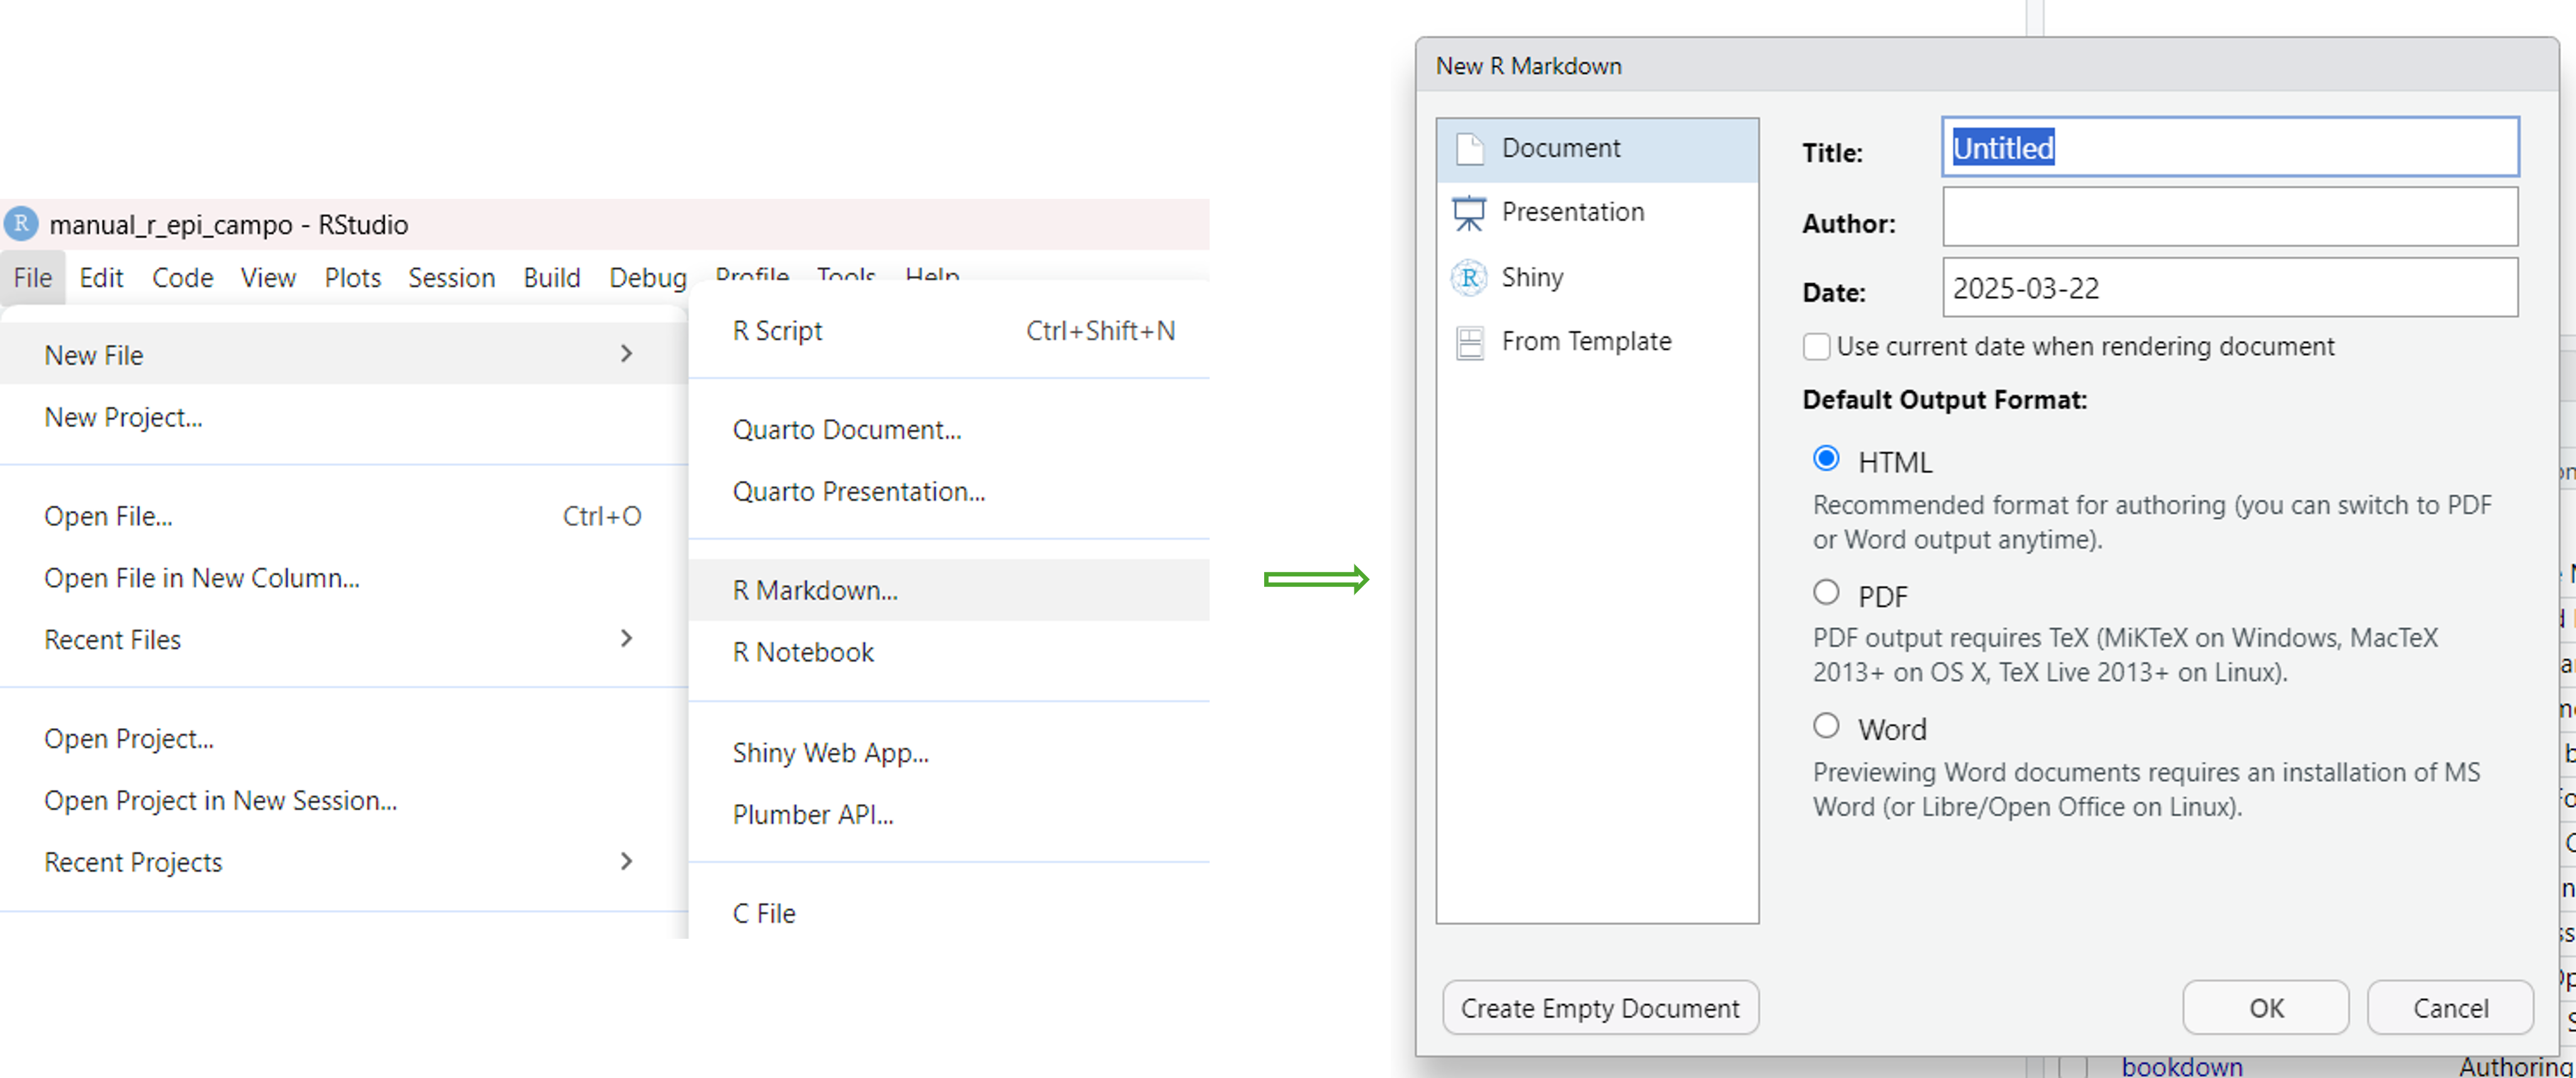
\includegraphics[keepaspectratio]{imagenes/08rmarkdown02.png}}

\section{Anatomía de un documento
RMarkdown}\label{anatomuxeda-de-un-documento-rmarkdown}

\pandocbounded{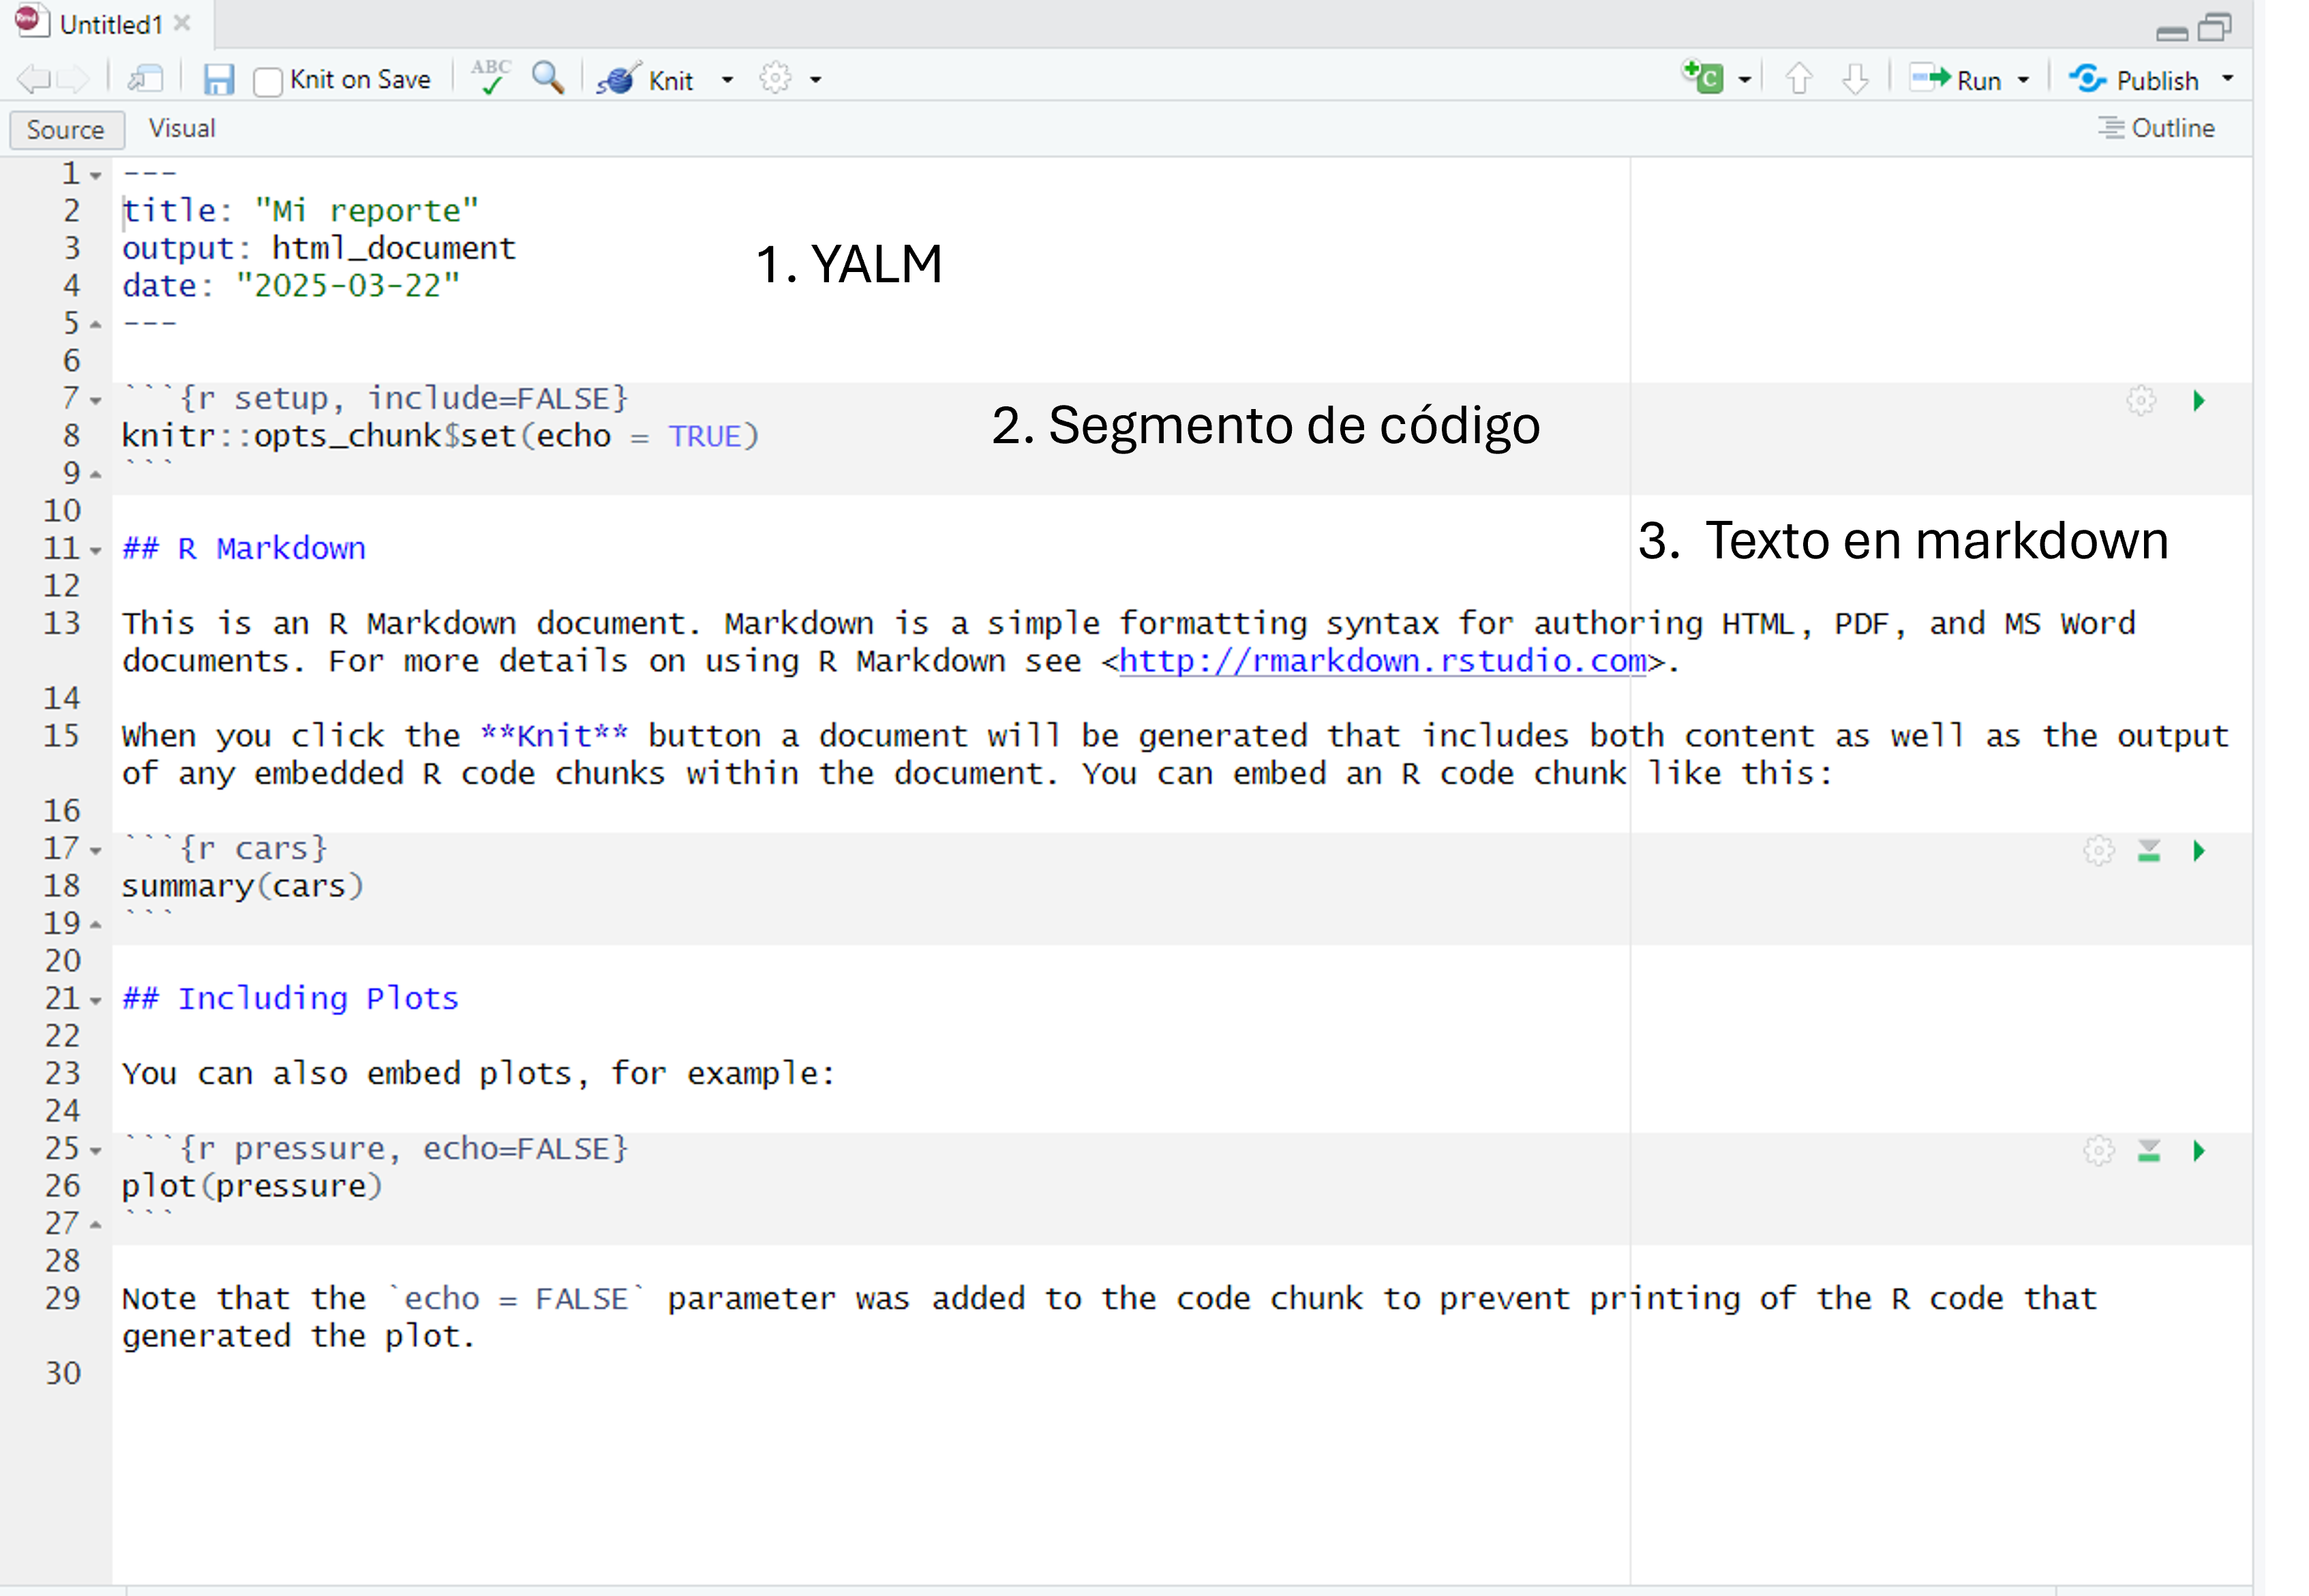
\includegraphics[keepaspectratio]{imagenes/08rmarkdown3.png}}

Ahora puedes guardar dentro de tu carpeta de proyecto esta plantilla en
formato \textbf{.rmd} (formato RMarkdown). Una recomendación a tener en
cuenta es tener todos los archivos asociados a este informe en RMarkdown
(base de datos, imágenes, etc.) estén en la misma carpeta del archivo
RMarkdown. También los documentos de salidas se generarán dentro de
esta.

Un documento RMarkdown tiene tres componentes principales:

\subsection{1. Encabezado YAML}\label{encabezado-yaml}

El encabezado YAML aparece al principio del documento entre líneas de
tres guiones (\texttt{-\/-\/-}).

\begin{Shaded}
\begin{Highlighting}[]
\PreprocessorTok{{-}{-}{-}}
\FunctionTok{title}\KeywordTok{:}\AttributeTok{ }\StringTok{"Análisis de Factores de Riesgo Cardiovascular"}
\FunctionTok{author}\KeywordTok{:}\AttributeTok{ }\StringTok{"Tu Nombre"}
\FunctionTok{date}\KeywordTok{:}\AttributeTok{ }\StringTok{"2025{-}03{-}22"}
\FunctionTok{output}\KeywordTok{:}\AttributeTok{ }
\AttributeTok{  }\FunctionTok{html\_document}\KeywordTok{:}
\AttributeTok{    }\FunctionTok{toc}\KeywordTok{:}\AttributeTok{ }\CharTok{true}
\AttributeTok{    }\FunctionTok{toc\_float}\KeywordTok{:}\AttributeTok{ }\CharTok{true}
\AttributeTok{    }\FunctionTok{theme}\KeywordTok{:}\AttributeTok{ united}
\PreprocessorTok{{-}{-}{-}}
\end{Highlighting}
\end{Shaded}

Este encabezado controla metadatos y opciones de formato. En el ejemplo,
especificamos un documento HTML con una tabla de contenidos flotante.

\subsection{2. segmentos de código
(chunks)}\label{segmentos-de-cuxf3digo-chunks}

Los bloques de código se definen entre triples acentos graves:

\begin{Shaded}
\begin{Highlighting}[]
\CommentTok{\# Tu código R aquí}
\end{Highlighting}
\end{Shaded}

Donde: - \texttt{nombre\_chunk}: Es un identificador único (opcional
pero recomendado) - \texttt{opciones}: Controlan cómo se ejecuta y
muestra el código

Algunas opciones comunes de los chunks:

\begin{itemize}
\tightlist
\item
  \texttt{echo\ =\ TRUE/FALSE}: Mostrar u ocultar el código
\item
  \texttt{eval\ =\ TRUE/FALSE}: Ejecutar o no el código
\item
  \texttt{warning\ =\ TRUE/FALSE}: Mostrar advertencias
\item
  \texttt{message\ =\ TRUE/FALSE}: Mostrar mensajes
\item
  \texttt{fig.width}/\texttt{fig.height}: Tamaño de gráficos
\item
  \texttt{include\ =\ TRUE/FALSE}: Incluir o no la salida en el
  documento final
\end{itemize}

Ejemplo de un bloque de código para análisis de datos de salud:

\begin{Shaded}
\begin{Highlighting}[]
\FunctionTok{library}\NormalTok{(tidyverse)}
\FunctionTok{library}\NormalTok{(readxl)}

\CommentTok{\# Cargar datos de pacientes}
\NormalTok{datos\_pacientes }\OtherTok{\textless{}{-}} \FunctionTok{read\_excel}\NormalTok{(}\StringTok{"datos\_hospital\_2024.xlsx"}\NormalTok{)}
\FunctionTok{glimpse}\NormalTok{(datos\_pacientes)}
\end{Highlighting}
\end{Shaded}

En la plantilla que creaste ahora, inserta varios segmentos de códigos
para que copies de los scripts que has creado lo vayas poniendo dentro
de estos, Ejemplo, en el primer segmento de código que tiene esta
plantilla,

\begin{Shaded}
\begin{Highlighting}[]
\NormalTok{knitr}\SpecialCharTok{::}\NormalTok{opts\_chunk}\SpecialCharTok{$}\FunctionTok{set}\NormalTok{(}\AttributeTok{echo =} \ConstantTok{TRUE}\NormalTok{)}
\end{Highlighting}
\end{Shaded}

pon el código para cargar los paquetes y también el código para cargar
las bases de datos.

En los demás segmentos, ve agregando las tablas que creaste usando
gtsummary o tabyl, los gráficos con ggplot.

\subsection{3. Texto narrativo en
markdown}\label{texto-narrativo-en-markdown}

El texto se escribe utilizando la sintaxis de Markdown, que permite
formatear fácilmente:

\begin{itemize}
\tightlist
\item
  \textbf{Encabezados}: \texttt{\#\ Encabezado\ 1},
  \texttt{\#\#\ Encabezado\ 2}, etc.
\item
  \textbf{Énfasis}: \texttt{*itálicas*} y \texttt{**negrita**}
\item
  \textbf{Listas}: Utilizando \texttt{-} o números
\item
  \textbf{Enlaces}: \texttt{{[}texto{]}(url)}
\item
  \textbf{Imágenes}: \texttt{!{[}texto\ alternativo{]}(ruta\_imagen)}
\item
  \textbf{Tablas}: Usando sintaxis de Markdown
\end{itemize}

Ejemplo de texto para un informe de salud:

\begin{Shaded}
\begin{Highlighting}[]
\DocumentationTok{\#\# Introducción}

\NormalTok{Este análisis examina la }\SpecialCharTok{**}\NormalTok{prevalencia de diabetes tipo }\DecValTok{2}\SpecialCharTok{**}\NormalTok{ en nuestra cohorte de pacientes durante el período }\DecValTok{2022}\FloatTok{{-}2024.} 

\NormalTok{Los factores de riesgo analizados incluyen}\SpecialCharTok{:}

\SpecialCharTok{{-}}\NormalTok{ Índice de masa }\FunctionTok{corporal}\NormalTok{ (IMC)}
\SpecialCharTok{{-}}\NormalTok{ Niveles de glucosa en ayunas}
\SpecialCharTok{{-}}\NormalTok{ Historial familiar}
\SpecialCharTok{{-}}\NormalTok{ Actividad física}
\end{Highlighting}
\end{Shaded}

\section{Buenas prácticas para RMarkdown en investigación de
salud}\label{buenas-pruxe1cticas-para-rmarkdown-en-investigaciuxf3n-de-salud}

\begin{enumerate}
\def\labelenumi{\arabic{enumi}.}
\tightlist
\item
  \textbf{Organiza tu código}: Usa chunks con nombres descriptivos y
  agrúpalos lógicamente.
\item
  \textbf{Documenta las decisiones analíticas}: Explica las
  transformaciones de datos y elecciones estadísticas.
\item
  \textbf{Controla la visibilidad del código}: Usa \texttt{echo=FALSE}
  para informes destinados a no-programadores.
\item
  \textbf{Incluye detalles metodológicos}: Documenta las versiones de
  los paquetes utilizados con \texttt{sessionInfo()}.
\item
  \textbf{Utiliza el control de versiones}: Guarda tus archivos .Rmd en
  un repositorio Git.
\item
  \textbf{Estructura clara}: Utiliza encabezados y subencabezados para
  organizar el contenido.
\item
  \textbf{Crea plantillas institucionales}: Desarrolla plantillas con
  los estilos y logotipos de tu institución.
\end{enumerate}

\section{Recursos adicionales para
profundizar}\label{recursos-adicionales-para-profundizar}

Para aprender más sobre RMarkdown en el contexto de análisis de datos en
salud:

\begin{itemize}
\tightlist
\item
  \href{https://bookdown.org/yihui/rmarkdown/}{R Markdown: The
  Definitive Guide}
\item
  \href{https://r4ds.had.co.nz/r-markdown.html}{R for Data Science}
\item
  \href{https://www.rstudio.com/resources/cheatsheets/}{RStudio
  RMarkdown Cheatsheet}
\item
  \href{https://bookdown.org/pdr_higgins/rmrwr/}{Reproducible Medical
  Research with R}
\item
  \href{https://www.epirhandbook.com/en/new_pages/rmarkdown.html}{R para
  epidemiólogos (capítulo de RMarkdown)}
\end{itemize}

\bookmarksetup{startatroot}

\chapter{Apendice}\label{apendice}

\section{Análisis de variables continuas - Estadistica (Ejemplos de
gráficos con
ggplot)}\label{anuxe1lisis-de-variables-continuas---estadistica-ejemplos-de-gruxe1ficos-con-ggplot}

\begin{Shaded}
\begin{Highlighting}[]
\NormalTok{knitr}\SpecialCharTok{::}\NormalTok{opts\_chunk}\SpecialCharTok{$}\FunctionTok{set}\NormalTok{(}\AttributeTok{echo =} \ConstantTok{TRUE}\NormalTok{,}
                      \AttributeTok{warning =} \ConstantTok{FALSE}\NormalTok{,}
                      \AttributeTok{message =} \ConstantTok{FALSE}\NormalTok{)}

\CommentTok{\#install.packages("readxl")}
\CommentTok{\#install.packages("tidyverse")}
\CommentTok{\#install.packages("knitr")}
\CommentTok{\#install.packages("kableExtra")}
\CommentTok{\#install.packages("ggpubr")}
\CommentTok{\#install.packages("dplyr")}
\CommentTok{\#install.packages("DescTools")}


\FunctionTok{library}\NormalTok{(readxl)}
\FunctionTok{library}\NormalTok{(tidyverse)}
\FunctionTok{library}\NormalTok{(knitr)}
\FunctionTok{library}\NormalTok{(kableExtra)}
\FunctionTok{library}\NormalTok{(ggplot2)}
\FunctionTok{library}\NormalTok{(DescTools)}
\FunctionTok{library}\NormalTok{(janitor)}

\DocumentationTok{\#\# Se recomienda ubicar aqui la lectura de los archivos y las librerias en este chunk.}
\DocumentationTok{\#\# It is recomended to put here the code to read the files and the libraries in this chunk.}
\DocumentationTok{\#\# VoÇe pode escrever a leitura dos arquivos e as livrarias nesse chunk.}

\CommentTok{\# Configurar la dirección de lectura de archivos.}
\CommentTok{\# Set the WORKING DIRECTORY}
\CommentTok{\#setwd("C:/Users/Julian/Documents/R/ANALISIS DE VAR CONTINUAS")}
\CommentTok{\#data \textless{}{-} read\_xlsx("AROMATICAS (Para desarrollar).xlsx")}


\NormalTok{data }\OtherTok{\textless{}{-}} \FunctionTok{read.csv}\NormalTok{(}\StringTok{"https://docs.google.com/spreadsheets/d/e/2PACX{-}1vT\_gIgjfKwvUOPAbK4kAa7rpRHFbQqm1wNoLAHhT4fJEZNLonTuysf3pYhU1MpEKg/pub?output=csv"}\NormalTok{, }\AttributeTok{dec =} \StringTok{","}\NormalTok{)}
\CommentTok{\# Mirar la línea 87 para cambiar los nombres de las variables.}

\CommentTok{\#Nota:En los siguientes enlaces, encuentra información sobre gráficos mejorados para analizar datos, principalmente relacionados con variables continuas.}
 \CommentTok{\# https://github.com/z3tt/beyond{-}bar{-}and{-}box{-}plots/blob/main/README.md?s=03}
\CommentTok{\#https://www.cedricscherer.com/slides/USGS{-}2021{-}beyond{-}bar{-}and{-}box{-}plots.pdf}
\end{Highlighting}
\end{Shaded}

\section{TABLA RESUMEN}\label{tabla-resumen}

En estas líneas puede escribir tu análisis.

\begin{Shaded}
\begin{Highlighting}[]
\CommentTok{\#Ejemplo para interpretar boxplot}
\CommentTok{\#https://rpubs.com/angiescetta/ejemplo{-}boxplot}

\NormalTok{data\_limpia }\OtherTok{\textless{}{-}}\NormalTok{ data }\SpecialCharTok{\%\textgreater{}\%} 
  \FunctionTok{clean\_names}\NormalTok{() }\SpecialCharTok{\%\textgreater{}\%} 
  \FunctionTok{rename}\NormalTok{(}\AttributeTok{Variable\_continua=}\NormalTok{velocidad,}
         \AttributeTok{Categoria=}\NormalTok{ciudad)}

\FunctionTok{glimpse}\NormalTok{(data\_limpia)}
\end{Highlighting}
\end{Shaded}

\begin{verbatim}
Rows: 60
Columns: 7
$ marca_temporal    <chr> "10/5/21 21:12", "10/5/21 21:14", "10/5/21 21:14", "~
$ Categoria         <chr> "Pereira", "Pereira", "Pereira", "Pereira", "Pereira~
$ lugar             <chr> "Viaducto", "Viaducto", "Viaducto", "Viaducto", "Via~
$ distancia_metros  <int> 300, 300, 300, 300, 300, 300, 100, 100, 100, 300, 30~
$ tiempo            <dbl> 16.73, 17.32, 15.01, 19.94, 14.69, 18.45, 7.73, 4.37~
$ velocidad_km_h    <dbl> 64.55469, 62.35566, 71.95203, 54.16249, 73.51940, 58~
$ Variable_continua <dbl> 64.6, 62.4, 72.0, 54.2, 73.5, 58.5, 46.6, 82.4, 68.8~
\end{verbatim}

\begin{Shaded}
\begin{Highlighting}[]
\FunctionTok{summary}\NormalTok{(data\_limpia)}
\end{Highlighting}
\end{Shaded}

\begin{verbatim}
 marca_temporal      Categoria            lugar           distancia_metros
 Length:60          Length:60          Length:60          Min.   :100     
 Class :character   Class :character   Class :character   1st Qu.:100     
 Mode  :character   Mode  :character   Mode  :character   Median :200     
                                                          Mean   :200     
                                                          3rd Qu.:300     
                                                          Max.   :300     
     tiempo       velocidad_km_h  Variable_continua
 Min.   : 4.370   Min.   :28.64   Min.   :28.60    
 1st Qu.: 7.022   1st Qu.:47.40   1st Qu.:47.42    
 Median :12.470   Median :59.93   Median :59.95    
 Mean   :12.450   Mean   :58.00   Mean   :58.26    
 3rd Qu.:17.148   3rd Qu.:68.32   3rd Qu.:68.65    
 Max.   :30.410   Max.   :93.99   Max.   :94.00    
\end{verbatim}

\begin{Shaded}
\begin{Highlighting}[]
\NormalTok{data\_limpia }\SpecialCharTok{\%\textgreater{}\%} \FunctionTok{group\_by}\NormalTok{(Categoria) }\SpecialCharTok{\%\textgreater{}\%}
  \FunctionTok{summarise}\NormalTok{(}\AttributeTok{count =} \FunctionTok{n}\NormalTok{(),}
  \AttributeTok{mode =} \FunctionTok{Mode}\NormalTok{(Variable\_continua),}
  \AttributeTok{mean\_media =} \FunctionTok{round}\NormalTok{(}\FunctionTok{mean}\NormalTok{(Variable\_continua, }\AttributeTok{na.rm =} \ConstantTok{TRUE}\NormalTok{), }\AttributeTok{digits =} \DecValTok{2}\NormalTok{),}
  \AttributeTok{min =}  \FunctionTok{min}\NormalTok{(Variable\_continua),}\AttributeTok{max =} \FunctionTok{max}\NormalTok{(Variable\_continua),}
  \AttributeTok{range =}\NormalTok{ max }\SpecialCharTok{{-}}\NormalTok{ min, }
  \AttributeTok{Q1 =} \FunctionTok{quantile}\NormalTok{(Variable\_continua, }\FloatTok{0.25}\NormalTok{),}
  \AttributeTok{median\_mediana =} \FunctionTok{median}\NormalTok{(Variable\_continua, }\AttributeTok{na.rm =} \ConstantTok{TRUE}\NormalTok{),}
  \AttributeTok{Q3 =} \FunctionTok{quantile}\NormalTok{(Variable\_continua, }\FloatTok{0.75}\NormalTok{),}
  \AttributeTok{IRC =}\NormalTok{ Q3 }\SpecialCharTok{{-}}\NormalTok{ Q1,}
  \AttributeTok{var =} \FunctionTok{round}\NormalTok{(}\FunctionTok{var}\NormalTok{(Variable\_continua),}\AttributeTok{digits =} \DecValTok{2}\NormalTok{),}
  \AttributeTok{sd =} \FunctionTok{round}\NormalTok{(}\FunctionTok{sd}\NormalTok{(Variable\_continua, }\AttributeTok{na.rm =} \ConstantTok{TRUE}\NormalTok{), }\AttributeTok{digits =} \DecValTok{2}\NormalTok{),}
  \AttributeTok{vc =} \FunctionTok{round}\NormalTok{(}\FunctionTok{sd}\NormalTok{(Variable\_continua, }\AttributeTok{na.rm =} \ConstantTok{TRUE}\NormalTok{) }\SpecialCharTok{/} \FunctionTok{mean}\NormalTok{(Variable\_continua, }\AttributeTok{na.rm =} \ConstantTok{TRUE}\NormalTok{),}\AttributeTok{digits =} \DecValTok{3}\NormalTok{),}
  \AttributeTok{P1 =} \FunctionTok{round}\NormalTok{((}\FunctionTok{mean}\NormalTok{(Variable\_continua, }\AttributeTok{na.rm =} \ConstantTok{TRUE}\NormalTok{) }\SpecialCharTok{{-}}\NormalTok{ mode)}\SpecialCharTok{/}\FunctionTok{sd}\NormalTok{(Variable\_continua, }\AttributeTok{na.rm =} \ConstantTok{TRUE}\NormalTok{),}\AttributeTok{digits =} \DecValTok{3}\NormalTok{),}
  \AttributeTok{P2 =} \FunctionTok{round}\NormalTok{((}\DecValTok{3}\SpecialCharTok{*}\NormalTok{(}\FunctionTok{mean}\NormalTok{(Variable\_continua, }\AttributeTok{na.rm =} \ConstantTok{TRUE}\NormalTok{) }\SpecialCharTok{{-}}\NormalTok{ median\_mediana))}\SpecialCharTok{/}\FunctionTok{sd}\NormalTok{(Variable\_continua, }\AttributeTok{na.rm =} \ConstantTok{TRUE}\NormalTok{),}\AttributeTok{digits=}\DecValTok{3}\NormalTok{)) }\SpecialCharTok{\%\textgreater{}\%} 
  \FunctionTok{kbl}\NormalTok{(}\AttributeTok{caption =} \StringTok{"Medidas de tendencia central y dispersion"}\NormalTok{,}
      \AttributeTok{align =} \StringTok{"lccrr"}\NormalTok{) }\SpecialCharTok{\%\textgreater{}\%} 
  \FunctionTok{kable\_classic}\NormalTok{(}\AttributeTok{full\_width =}\NormalTok{ F, }\AttributeTok{html\_font =} \StringTok{"Cambria"}\NormalTok{)}
\end{Highlighting}
\end{Shaded}

\begin{table}
\centering
\caption{Medidas de tendencia central y dispersion}
\centering
\begin{tabular}[t]{l|c|c|r|r|l|c|c|r|r|l|c|c|r|r|l}
\hline
Categoria & count & mode & mean\_media & min & max & range & Q1 & median\_mediana & Q3 & IRC & var & sd & vc & P1 & P2\\
\hline
Pereira & 40 & 71.9 & 61.21 & 33.1 & 82.4 & 49.3 & 56.525 & 61.95 & 69.375 & 12.85 & 145.01 & 12.04 & 0.197 & -0.888 & -0.184\\
\hline
Santa Rosa de Cabal & 20 & NA & 52.35 & 28.6 & 94.0 & 65.4 & 35.550 & 48.45 & 64.450 & 28.90 & 394.49 & 19.86 & 0.379 & NA & 0.590\\
\hline
\end{tabular}
\end{table}

\section{GRÁFICO DE CAJAS - BOX
PLOT}\label{gruxe1fico-de-cajas---box-plot}

\begin{Shaded}
\begin{Highlighting}[]
\CommentTok{\# En este y los demas "chunks" que cree ubicara el codigo para procesar los datos y generar las tablas y graficos.}

\CommentTok{\#Nota:En los siguientes enlaces, encuentra información sobre gráficos mejorados para analizar datos, principalmente relacionados con variables continuas.}
 \CommentTok{\# https://github.com/z3tt/beyond{-}bar{-}and{-}box{-}plots/blob/main/README.md?s=03}
\CommentTok{\#https://www.cedricscherer.com/slides/USGS{-}2021{-}beyond{-}bar{-}and{-}box{-}plots.pdf}

\DocumentationTok{\#\# La siguiente forma de realizar el BOXPLOT permite filtrar los datos más facil, está escrito en modo de sintaxis TYDIVERSE y facilita la manipulación del gráfico.}
\NormalTok{data\_limpia }\SpecialCharTok{\%\textgreater{}\%} 
  \FunctionTok{ggplot}\NormalTok{(}\FunctionTok{aes}\NormalTok{(}\AttributeTok{y=}\NormalTok{ Variable\_continua , }\AttributeTok{x=}\NormalTok{ Categoria))}\SpecialCharTok{+}
    \FunctionTok{geom\_boxplot}\NormalTok{()}\SpecialCharTok{+}
  \FunctionTok{labs}\NormalTok{(}\AttributeTok{title =} \StringTok{"Gráfico de cajas para la variable continua de acuerdo a la categoria"}\NormalTok{,}
       \AttributeTok{caption =} \StringTok{"El diamante negro representa la ubicación de la media"}\NormalTok{)}
\end{Highlighting}
\end{Shaded}

\pandocbounded{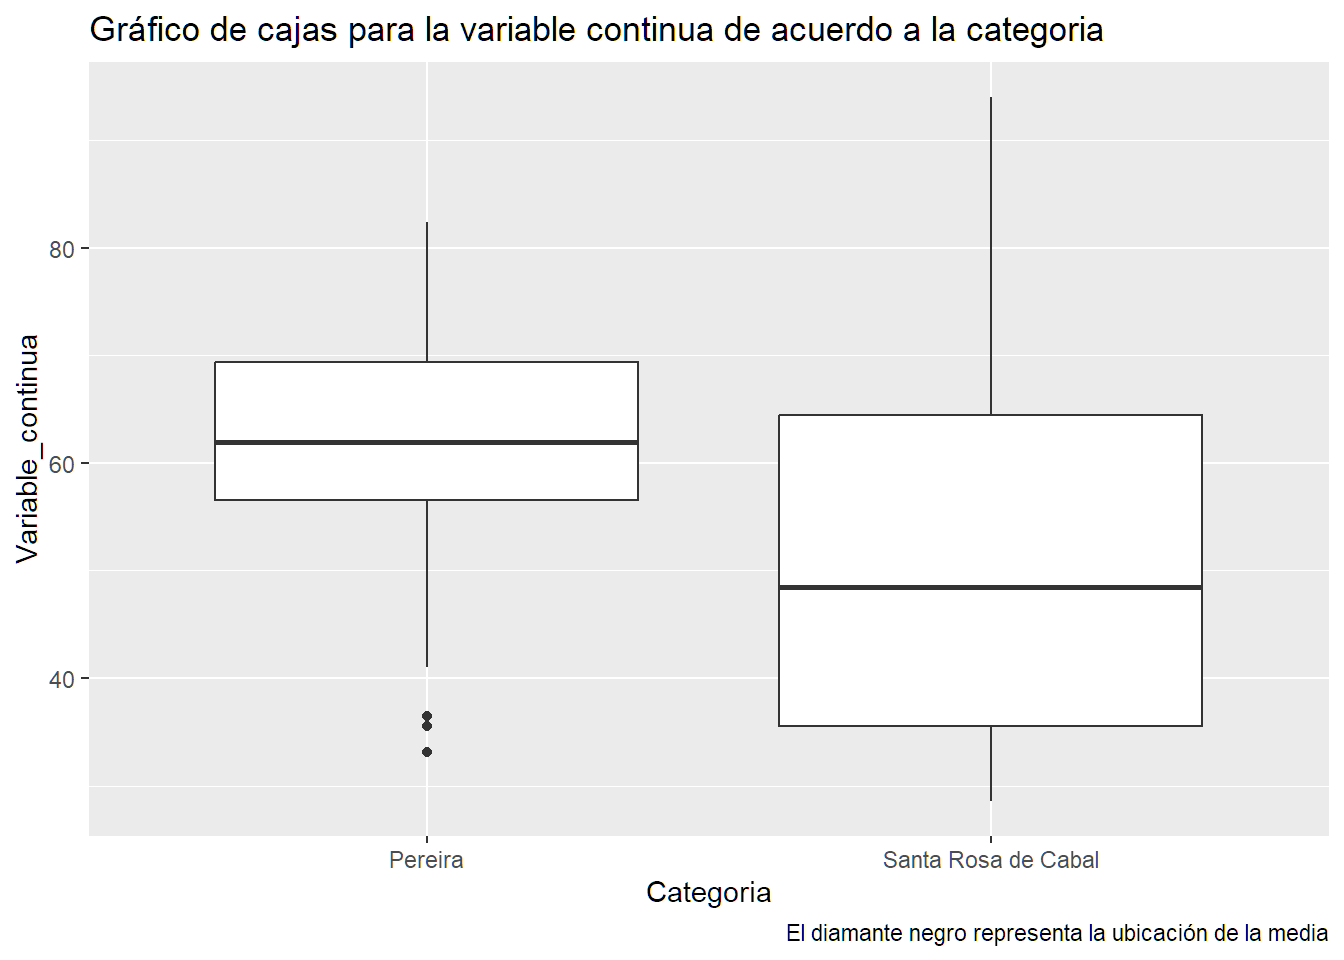
\includegraphics[keepaspectratio]{08-analisisEstadistico_files/figure-pdf/BOXPLOT-1.pdf}}

\section{GRÁFICOS DE DENSIDAD}\label{gruxe1ficos-de-densidad}

En estas líneas puede escribir sus análisis.

\begin{Shaded}
\begin{Highlighting}[]
\CommentTok{\# En este y los demas "chunks" que cree ubicara el codigo para procesar los datos y generar las tablas y graficos.}


\NormalTok{data\_limpia }\SpecialCharTok{\%\textgreater{}\%} 
  \FunctionTok{ggplot}\NormalTok{(}\FunctionTok{aes}\NormalTok{(}\AttributeTok{x=}\NormalTok{ Variable\_continua))}\SpecialCharTok{+}
  \FunctionTok{geom\_density}\NormalTok{() }\SpecialCharTok{+}
  \FunctionTok{labs}\NormalTok{(}\AttributeTok{title =} \StringTok{"Gráfico de densidad"}\NormalTok{,}
       \AttributeTok{subtitle =} \StringTok{"Por categorias"}\NormalTok{) }\SpecialCharTok{+}
  \FunctionTok{facet\_grid}\NormalTok{(Categoria }\SpecialCharTok{\textasciitilde{}}\NormalTok{. )}
\end{Highlighting}
\end{Shaded}

\pandocbounded{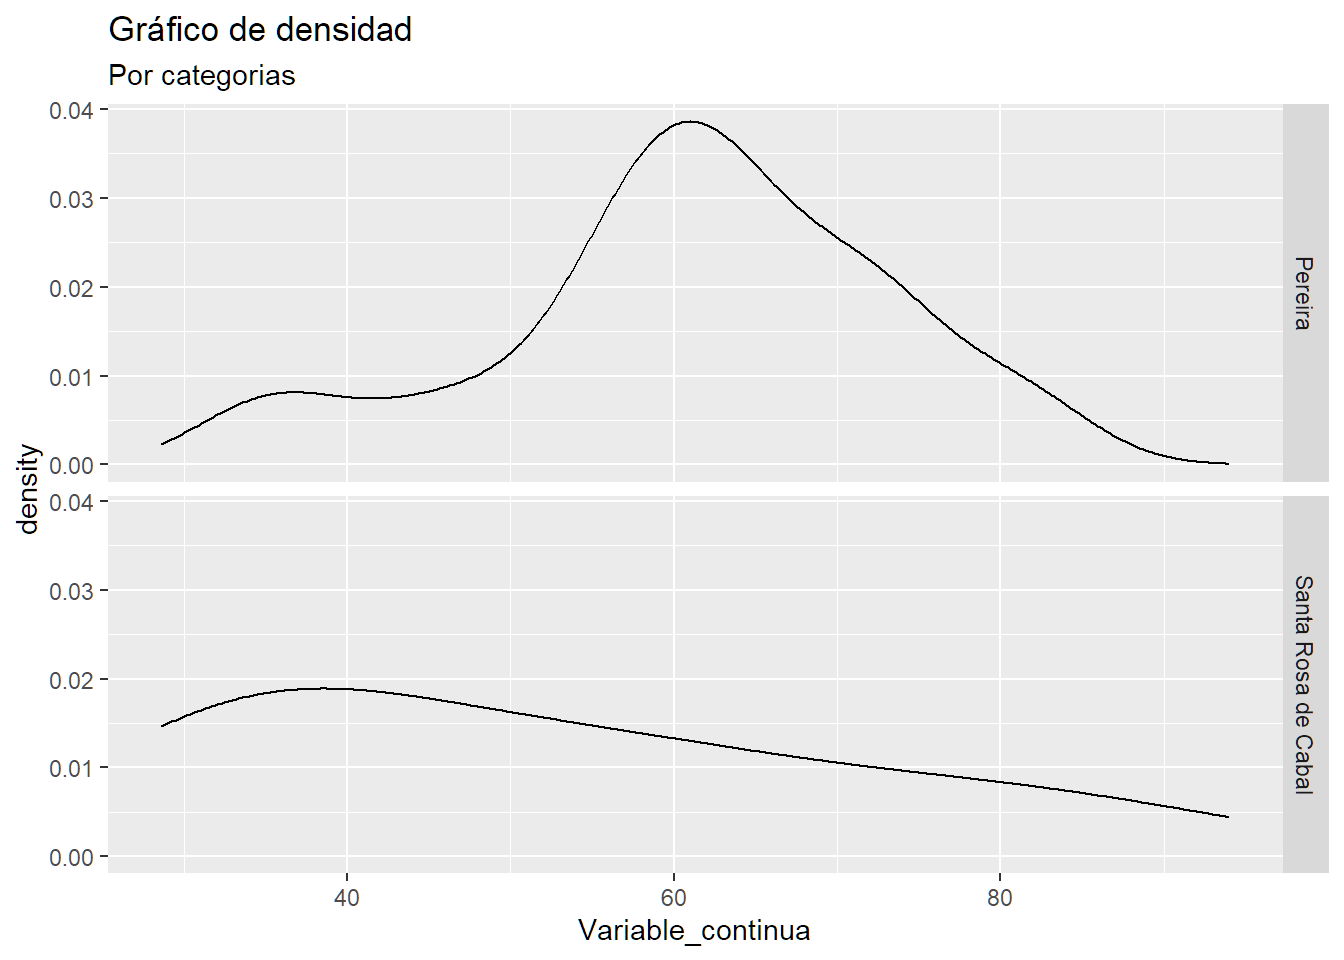
\includegraphics[keepaspectratio]{08-analisisEstadistico_files/figure-pdf/DENSITY-1.pdf}}

\begin{Shaded}
\begin{Highlighting}[]
\CommentTok{\#Estas lineas sirven para crear el gráfico de densidad para una categoria individual}
\CommentTok{\#data \%\textgreater{}\% }
\CommentTok{\# filter(Categoria == "MENTA") \%\textgreater{}\% }
\CommentTok{\# ggplot(aes(x= Variable\_continua))+}
\CommentTok{\# geom\_density()+}
\CommentTok{\# labs(title = "MENTA",}
\CommentTok{\# subtitle = "Gráfico de densidad")}
\end{Highlighting}
\end{Shaded}

\section{HISTOGRAMAS}\label{histogramas}

En estas líneas puede escribir sus análisis.

\begin{Shaded}
\begin{Highlighting}[]
\CommentTok{\#Estas lineas sirven para crear el histograma para una categoria individual}
  \CommentTok{\#Con el binwidth se puede ajustar el ancho de las barras, puede explorar}
  \CommentTok{\# un poco con los anchos, aunque.}
  \CommentTok{\# La ley de STURGES permite calcular el número de clases y así el ancho de clase adecuado para    \#gráficar un histograma de   manera técnica.}

\NormalTok{data\_limpia }\SpecialCharTok{\%\textgreater{}\%} 
  \FunctionTok{ggplot}\NormalTok{(}\FunctionTok{aes}\NormalTok{(}\AttributeTok{x=}\NormalTok{ Variable\_continua))}\SpecialCharTok{+}
  \FunctionTok{geom\_histogram}\NormalTok{(}\AttributeTok{binwidth =} \FloatTok{2.5}\NormalTok{)}\SpecialCharTok{+}
  \FunctionTok{labs}\NormalTok{(}\AttributeTok{title =} \StringTok{"HIERBA BUENA"}\NormalTok{,}
       \AttributeTok{subtitle =} \StringTok{"Histograma"}\NormalTok{)}\SpecialCharTok{+}
  \FunctionTok{facet\_grid}\NormalTok{(Categoria }\SpecialCharTok{\textasciitilde{}}\NormalTok{. )}
\end{Highlighting}
\end{Shaded}

\pandocbounded{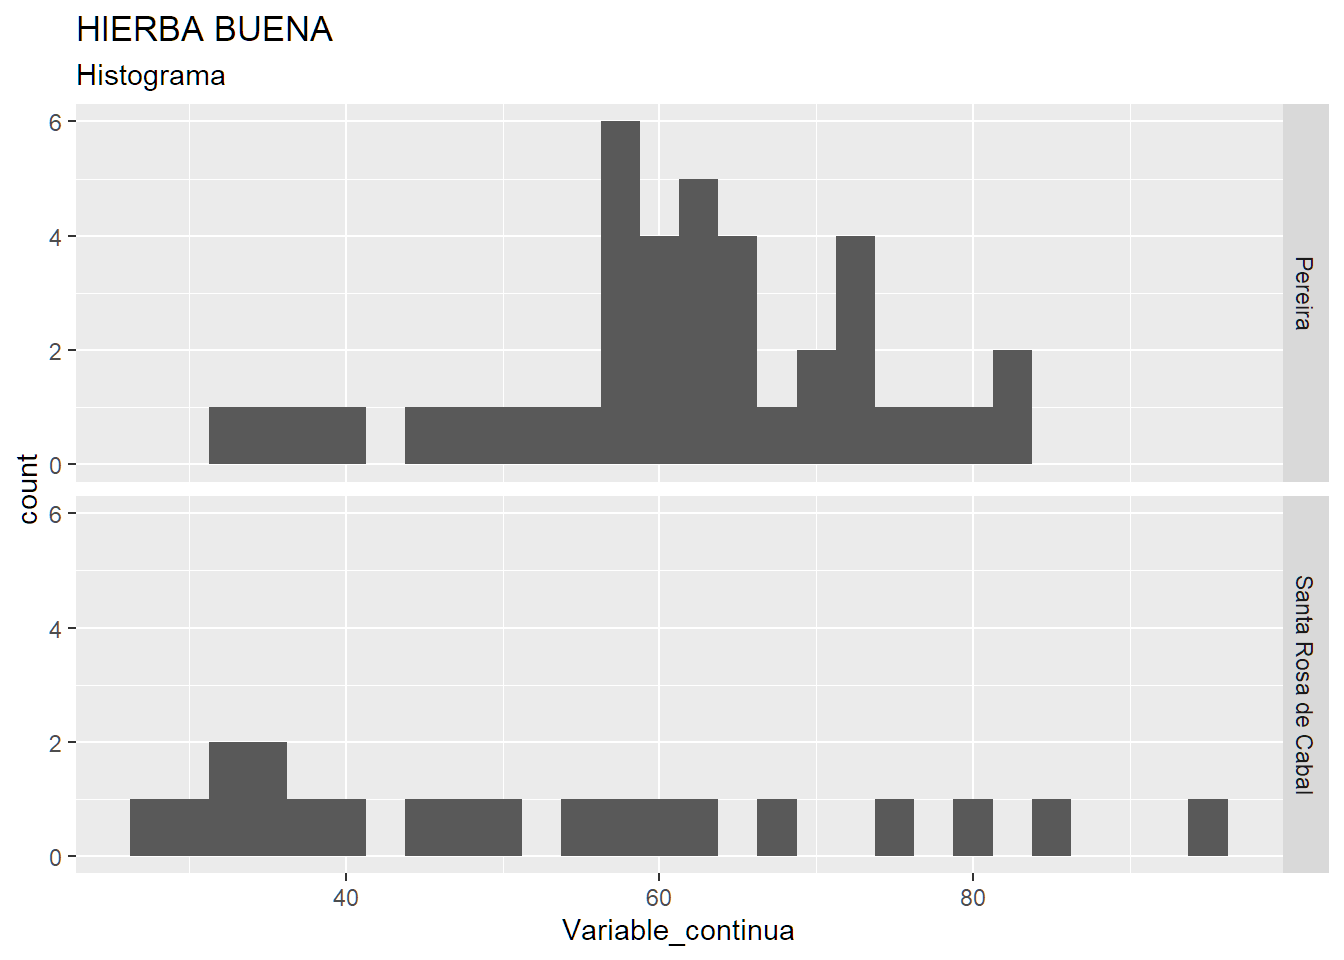
\includegraphics[keepaspectratio]{08-analisisEstadistico_files/figure-pdf/HISTOGRAMA-1.pdf}}

\begin{Shaded}
\begin{Highlighting}[]
\CommentTok{\#Estas lineas sirven para crear el histograma para una categoria individual}
\CommentTok{\# data \%\textgreater{}\% }
\CommentTok{\#   filter(Categoria == "MENTA") \%\textgreater{}\% }
\CommentTok{\#   ggplot(aes(x= Variable\_continua))+}
\CommentTok{\#   geom\_histogram(binwidth = 1)+}
\CommentTok{\#   labs(title = "MENTA",}
\CommentTok{\#   subtitle = "Histograma")}
\end{Highlighting}
\end{Shaded}

\section{HISTOGRAMAS Y GRÁFICOS DE
DENSIDAD.}\label{histogramas-y-gruxe1ficos-de-densidad.}

En estas líneas puede escribir sus análisis.

\begin{Shaded}
\begin{Highlighting}[]
\NormalTok{data\_limpia }\SpecialCharTok{\%\textgreater{}\%} 
  \FunctionTok{ggplot}\NormalTok{(}\FunctionTok{aes}\NormalTok{(}\AttributeTok{x=}\NormalTok{ Variable\_continua, }\AttributeTok{y=}\NormalTok{ ..density..))}\SpecialCharTok{+}
  \FunctionTok{geom\_histogram}\NormalTok{(}\AttributeTok{binwidth =} \DecValTok{2}\NormalTok{)}\SpecialCharTok{+}
  \FunctionTok{geom\_density}\NormalTok{()}\SpecialCharTok{+}
  \FunctionTok{facet\_grid}\NormalTok{(Categoria }\SpecialCharTok{\textasciitilde{}}\NormalTok{. )}
\end{Highlighting}
\end{Shaded}

\begin{verbatim}
Warning: The dot-dot notation (`..density..`) was deprecated in ggplot2 3.4.0.
i Please use `after_stat(density)` instead.
\end{verbatim}

\pandocbounded{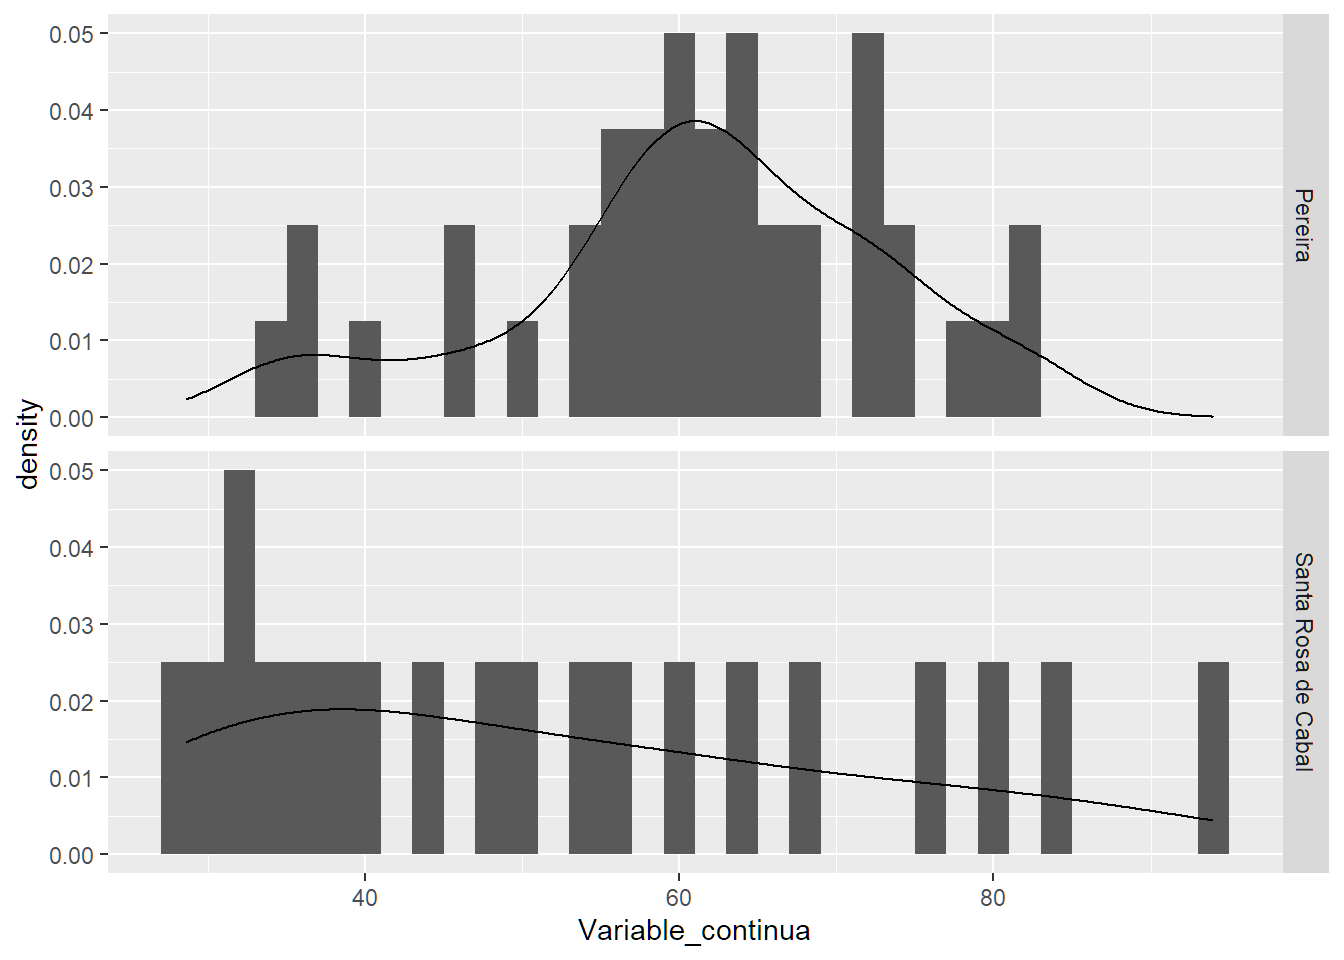
\includegraphics[keepaspectratio]{08-analisisEstadistico_files/figure-pdf/DENSITY_HIS-1.pdf}}

\begin{Shaded}
\begin{Highlighting}[]
\CommentTok{\#Estas lineas sirven para crear el histograma para una categoria individual}
  \CommentTok{\#Con el binwidth se puede ajustar el ancho de las barras, puede explorar}
  \CommentTok{\# un poco con los anchos, aunque.}
  \CommentTok{\# La ley de STURGES permite calcular el número de clases y así el ancho de clase adecuado para    \#gráficar un histograma de   manera técnica.}
  
\CommentTok{\#data \%\textgreater{}\% }
\CommentTok{\#filter(Categoria == "MENTA") \%\textgreater{}\% }
\CommentTok{\#ggplot(aes(x= Variable\_continua, y= ..density..))+}
\CommentTok{\#geom\_histogram(binwidth = 1.5)+}
\CommentTok{\#geom\_density()}
\end{Highlighting}
\end{Shaded}

\bookmarksetup{startatroot}

\chapter*{Referencias}\label{referencias}
\addcontentsline{toc}{chapter}{Referencias}

\markboth{Referencias}{Referencias}

\phantomsection\label{refs}
\begin{CSLReferences}{1}{0}
\bibitem[\citeproctext]{ref-aragon_epitools_2020}
Aragon, Tomas J., Michael P. Fay, Daniel Wollschlaeger, and Adam
Omidpanah. 2020. {``Epitools: {Epidemiology} {Tools}.''}
\url{https://cran.r-project.org/web/packages/epitools/index.html}.

\bibitem[\citeproctext]{ref-schauberger_openxlsx_2023}
Schauberger, Philipp, Alexander Walker, Luca Braglia, Joshua Sturm, Jan
Marvin Garbuszus, and Jordan Mark Barbone. 2023. {``Openxlsx: {Read},
{Write} and {Edit} Xlsx {Files}.''}
\url{https://cran.r-project.org/web/packages/openxlsx/index.html}.

\bibitem[\citeproctext]{ref-spina_epikit_2023}
Spina, Alexander, Zhian N. Kamvar, Dirk Schumacher, and Kate Doyle.
2023. {``Epikit: {Miscellaneous} {Helper} {Tools} for
{Epidemiologists}.''}
\url{https://cran.r-project.org/web/packages/epikit/index.html}.

\bibitem[\citeproctext]{ref-vega}
Vega, Juan Bosco Mendoza. n.d. \emph{R Para Principiantes}.
\url{https://bookdown.org/jboscomendoza/r-principiantes4/}.

\bibitem[\citeproctext]{ref-waring2022}
Waring, Elin, Michael Quinn, Amelia McNamara, Eduardo Arino de la Rubia,
Hao Zhu, Julia Lowndes, Shannon Ellis, et al. 2022. \emph{Skimr: Compact
and Flexible Summaries of Data}.
\url{https://cran.r-project.org/web/packages/skimr/index.html}.

\bibitem[\citeproctext]{ref-wickham_tidyverse_2023}
Wickham, Hadley, and RStudio. 2023. {``Tidyverse: {Easily} {Install} and
{Load} the '{Tidyverse}'.''}
\url{https://cran.r-project.org/web/packages/tidyverse/index.html}.

\end{CSLReferences}




\end{document}
